
\documentclass[a4paper,10pt]{article}

%%% ---------------- %%%
% LaTeX heeft een zekere basisfunctionaliteit maar meestal is deze onvoldoende. Daarvoor bestaan er bijkomende pakketten.
%
% P.S. In een regel is alles na '%' een opmerking. Deze worden niet opgenomen bij compilatie van het document.
%%% ---------------- %%%

\usepackage[english]{babel}   % Spellingcorrectie en titels in NL
\usepackage[pdftex]{graphicx}       % Pakket voor afbeeldingen
\usepackage{longtable}
\usepackage[colorlinks, linkcolor=black, citecolor=black, urlcolor=black]{hyperref}
\usepackage{geometry}       % Pakket voor pagina-indeling
\geometry{tmargin=3cm, bmargin=2.2cm, lmargin=2.2cm, rmargin=2cm}
\usepackage{todonotes}      % Pakket voor figuur 'placeholders'
\usepackage{subcaption}
\usepackage{ifthen}
\usepackage{enumitem}
\usepackage{amsmath}        % Pakket voor vergelijkingen
\usepackage{floatrow}
\usepackage{amsmath, amssymb, amsthm}
\usepackage{listings}
\usepackage{xcolor}
\usepackage{siunitx}
\usepackage{hhline}
\definecolor{backcolour}{rgb}{0.95,0.95,0.92}
\lstdefinestyle{mystyle}{backgroundcolor=\color{backcolour},  language=Matlab }
\lstset{style=mystyle}
\floatsetup[table]{capposition=top}     % Pakket dat bovenschriften creëert bij tabellen ipv de standaard onderschriften.
\usepackage{float}
\usepackage{svg}
\usepackage{wasysym}
\usepackage{framed}
\usepackage{lscape}
\usepackage{array}
\usepackage{bold-extra}
\newcommand{\textbox}[2][6]{
\begin{framed}
\noindent#2
\end{framed}}
\usepackage[toc,page]{appendix}

\usepackage{acro}
\acsetup{list/template=tabular, format/short = \scshape}

\DeclareAcronym{os}{
  short={os},
  long=Operating System
}
\DeclareAcronym{mvc}{
  short={mvc},
  long=Model-View-Controller,
}
\DeclareAcronym{orm}{
  short={orm},
  long=Object Relational Mapper,
}
\DeclareAcronym{http}{
  short={http},
  long=HyperText Transport Protocol,
}
\DeclareAcronym{https}{
  short={https},
  long=HyperText Transport Protocol Secure,
}
\DeclareAcronym{html}{
  short={html},
  long=HyperText Markup Language,
}
\DeclareAcronym{ssl}{
  short={ssl},
  long=Secure Socket Layer,
}
\DeclareAcronym{tls}{
  short={tls},
  long=Transport Layer Security,
}
\DeclareAcronym{wsgi}{
  short={wsgi},
  long=Web Server Gateway Interface,
}
\DeclareAcronym{vpn}{
  short={vpn},
  long=Virtual Private Network,
}
\DeclareAcronym{rest}{
  short={rest},
  long=Representational State Transfer,
}
\DeclareAcronym{api}{
  short={api},
  long=Application Programming Interface,
}
\DeclareAcronym{json}{
  short={json},
  long=JavaScript Object Notation,
}
\DeclareAcronym{anpr}{
  short={anpr},
  long=Automatic Number Plate Recognition,
}
\DeclareAcronym{udms}{
  short={udms},
  long=Ultrasonic Distance Measuring Sensor,
}
\DeclareAcronym{iot}{
  short={IoT},
  long=Internet of Things,
}
\DeclareAcronym{mp}{
  short={mp},
  long=Mega Pixel,
}
\DeclareAcronym{cpu}{
short={cpu},
long=Central Processing Unit,
}
\DeclareAcronym{ram}{
short={ram},
long=Random Access Memory
}
\DeclareAcronym{sql}{
short={sql},
long=Structured Query Language
}
\DeclareAcronym{rdbms}{
short={rdbms},
long=Relational Database Management System 
}
\DeclareAcronym{ocr}{
short={ocr},
long=Optical Character Recognition
}
\DeclareAcronym{gdpr}{
short=gdpr,
long=General Data Protection Regulation
}
\DeclareAcronym{js}{
short=js,
long=JavaScript
}
\DeclareAcronym{lan}{
short=lan,
long=Local Area Network
}
\DeclareAcronym{gui}{
short=gui,
long=Graphical User Interface
}
\DeclareAcronym{ips}{
short=ips,
long=Intelligent Parking System
}
\DeclareAcronym{ddos}{
short=ddos,
long=Distributed Denial of Server
}
\DeclareAcronym{csrf}{
short=csrf,
long=Cross Site Request Forgery
}
\DeclareAcronym{idor}{
short=idor,
long=Indirect Object Reference
}
\DeclareAcronym{lcd}{
short=lcd,
long=Liquid Crystal Display
}
\DeclareAcronym{2fa}{
short=2fa,
long=Two Factor Authentication
}
\DeclareAcronym{rce}{
short=rce,
long=Remote Code Execution
}
\DeclareAcronym{xss}{
short=xss,
long=Cross Site Scripting
}
\DeclareAcronym{acl}{
short=acl,
long=Access Control Level
}
\DeclareAcronym{ssrf}{
short=ssrf,
long=Server-Side Request Forgery
}
\DeclareAcronym{jwt}{
short=jwt,
long=\textsc{json} Web Tokens
}
\DeclareAcronym{totp}{
short=totp,
long=Timed One Time Password
}
\DeclareAcronym{led}{
short=led,
long= Light Emitting Diode
}
\DeclareAcronym{mdf}{
short=mdf,
long= Medium Density Fibreboard
}
\DeclareAcronym{url}{
short=url,
long= Uniform Resource Locator
}
\DeclareAcronym{wifi}{
short=WiFi,
long= Wireless Fidelity,
short-format = \rmfamily ,
}
\DeclareAcronym{apm}{
short=apm,
long= Application Performance Monitoring,
}
\DeclareAcronym{cvc}{
short=cvc,
long= Card Validation Code,
}
\DeclareAcronym{qr}{
short=qr,
long= Quick Response,
}
\DeclareAcronym{acm}{
short=acm,
long= Access Control Misconfiguration,
}
\DeclareAcronym{mitm}{
short=mitm,
long= Man In The Middle,
}
\DeclareAcronym{tpa}{
short=tpa,
long= Third-Party Authenticator,
}
\DeclareAcronym{cdn}{
short=cdn,
long= Content Delivery Network,
}

\DeclareAcronym{dos}{
short=dos,
long= Denial of Service,
}

\usepackage{tocloft}
\usepackage{comment}

\newlength{\mylen}
\setlength{\mylen}{5px}

\newlength{\figlen}
\setlength{\figlen}{10px}

\renewcommand{\cftfigpresnum}{\figurename\enspace}
\renewcommand{\cftfigaftersnum}{:}
\settowidth{\figlen}{\cftfigpresnum\cftfigaftersnum}
\renewcommand{\cftsecleader}{\cftdotfill{\cftdotsep}}
\addtolength{\cftfignumwidth}{25px}

\renewcommand{\cfttabpresnum}{\tablename\enspace}
\renewcommand{\cfttabaftersnum}{:}
\settowidth{\mylen}{\cfttabpresnum\cfttabaftersnum}
\renewcommand{\cftsecleader}{\cftdotfill{\cftdotsep}}
\addtolength{\cfttabnumwidth}{25px}
\newcommand{\tabitem}{~~\llap{\textbullet}~~}

\setlength\parindent{1em}
\newcommand{\ind}{\hspace{1.2em}}

\usepackage{titlesec}
\usepackage{float}
\usepackage[labelfont=bf,format=hang]{caption}
\captionsetup{labelfont=bf}

\setcounter{secnumdepth}{4}

\titleformat{\paragraph}
{\normalfont\normalsize\bfseries}{\theparagraph}{1em}{}
\titlespacing*{\paragraph}
{0pt}{3.25ex plus 1ex minus .2ex}{1.5ex plus .2ex}


\begin{document}
\begin{titlepage}
    \newpage
    \pagenumbering{Roman}
    \thispagestyle{empty}
    \frenchspacing
    \hspace{-0.2cm}
    \hspace{0.2cm}
    \hspace{0.2cm}
    
\includegraphics[height=2.5cm]{images/logoFirW.jpg}
    \hspace{5.8cm}
    
\includegraphics[height=2.5cm]{images/kul_logo.jpg}
    %\begin{minipage}[b]{8cm}
        %\Large{Katholieke\newline Universiteit\newline Leuven}\smallskip\newline
        %\large{}\smallskip\newline
        %\textbf{Faculteit\newline Ingenieurswetenschappen}\smallskip
    %\end{minipage}
    \hspace{\stretch{1}}
    \vfill
    \vspace{0.5cm}
    \centering\Large{\rm\textbf{{Problem Solving and Engineering Design part 3}}}
    \vspace*{0.5cm}\vfill
    \begin{center}
        \begin{minipage}[t]{\textwidth}
            \begin{center}
                \Large{\rm{\textbf{CW1B2}}}\\
                \vspace{0.3cm}
                \normalsize{\rm {Ruben Mariën (r0883561)}}\\
                {\rm {Robin Martens (r0885874)}}\\
                {\rm {Neel Van Den Brande (r0876234)}}\\
                {\rm {Rik Vanhees (r0885864)}}\\
                {\rm {Rune Verachtert (r0884615)}}\\
                {\rm {Tuur Vernieuwe (r0886802)}}\\
                \vspace{2.5cm}
                
                \Huge{\rm\textbf{An intelligent parking garage}} \\
                \vspace{1cm}
                \large{\rm\textsc{{preliminary report}}} \\
                \vspace{4cm}
                {\rm \large\underline{Co-titular}} \\
                {\rm \normalsize{prof. dr. ir. Bart De Decker}} \\
                \vspace{0.5cm}
                {\rm \large\underline{Coaches}} \\
                {\rm \normalsize{Shuaibu Musa Adam}} \\
                {\rm \normalsize{Shirin Kalantari}} \\
                {\rm \normalsize{Hamdi Trimech}} \\
                \vspace{1.5cm}
                \LARGE{\rm\textsc{academic year 2022-2023}}
                \vfill
            \end{center}
        \end{minipage}
    \end{center}
    \vfill
\end{titlepage}

\vspace*{\fill} % for vertical centering 1/3

\textbox{
\begin{center}
    \textit{\textbf{Declaration of originality}}
\end{center}

\noindent \textit{We hereby declare that this submitted draft is entirely our own, subject to feedback and support given us by the didactic team, and subject to lawful cooperation which was agreed with the same didactic team.}
\textit{Regarding this draft, we also declare that:}

\begin{enumerate}
    \item \textit{Note has been taken of the text on academic integrity (\url{https://eng.kuleuven.be/studeren/masterproef-en-papers/documenten/20161221-academischeintegriteit-okt2016.pdf}).}
    \item \textit{No plagiarism has been committed as described on \url{https://eng.kuleuven.be/studeren/masterproef-en-papers/plagiaat}.}
    \item \textit{All experiments, tests, measurements, …, have been performed as described in this draft, and no data or measurement results have been manipulated.}
    \item \textit{All sources employed in this draft – including internet sources – have been correctly referenced.}
\end{enumerate}

\noindent \textit{This we solemnly declare, in our own free will and on our own word of honor.} 
}
\vspace*{\fill}
\vspace{\baselineskip}


\newpage
\begin{abstract}
Nowadays, time has become more of the essence, so people value efficiency on all fronts highly. This project was aimed at developing an efficient and intelligent parking garage with an automatic payment and reservation tool. Sadly, often this efficiency comes at the expense of the user's privacy. That is why this paper also looks into the question: ``How can a garage be as secure as possible, without reducing its efficiency?"

A scale model of a real life parking garage was built alongside a functional application, to deliver a proof of concept in this report. Via usage of automatic number plate recognition and internet of things devices, the garage is able to detect entering and leaving cars and calculate the amount each car owner has to pay. This payment can happen automatically, but only if allowed by the user. Via a self built application the user can make reservations for a garage, see the available parking lots at any time and activate or pay the garage bills. The entire system is built with privacy and security as its primary goal.
\end{abstract}
\clearpage

\addcontentsline{toc}{section}{Contents}
\tableofcontents
\clearpage

\addcontentsline{toc}{section}{\listfigurename}
\listoffigures

\clearpage
\addcontentsline{toc}{section}{\listtablename}
\listoftables

\clearpage
\addcontentsline{toc}{section}{List of Acronyms}
\acsetup{format/short=\MakeUppercase}
\printacronyms[name=List of Abbreviations]
\acsetup{format/short=\scshape}

\newpage

\pagenumbering{arabic}
\setcounter{page}{1}
\newpage


\section{Introduction}\label{Introduction}

% Brede context + versmalling
People these days value efficiency in life on all fronts higher than ever. Time has become more and more valuable. Almost every family owns a car with most of them even owning two or three \cite{vehicles_in_families}, and travelling by car has become increasingly popular. Therefore, parking efficiency is an element that affects everyone on a near daily basis. This requires engineers to invent and examine new solutions to improve this parking experience. The dissatisfaction with the classic ticket system in most parking garages, causes an evolution into more digital and automated systems. Often accomplished through licence plate recognition in combination with mobile apps and automated payment options \cite{4411}. Despite the convenience of these systems, it poses a risk of a privacy breach \cite{privacy_breach}. Therefore, sufficient attention should be given to the security of these systems. The privacy of the user is the number one priority.\\

% Doel
The main goal of the project is to make an automatic parking garage using \ac{iot} devices. This means that a client will be able to drive into the garage and park his/her car there for a certain duration of time. Then, drive away without having to pay with the use of a ticket. This is accomplished by cameras and \ac{anpr} software, together with a mobile application. \\

This report describes both the mechanical and software aspects of the design. Section \ref{sec:general design} describes the working of the entire system in an abstract way. Section \ref{sec:implementation} gives the concrete implementation of the system. The reasons why the components of the system were chosen can be found in section \ref{sec:design-motivation}. Then, section \ref{sec:case-example} describes a sample user experience in the \ac{ips}. Next, section \ref{sec:system analysis} gives a critical analysis of the final system. Section \ref{sec:conclusion} gives a conclusion of the project and finally, Section \ref{sec:course-integration} gives an overview of the course integration with the different courses in the first and second year of the Bachelor in Engineering Science.

%Section \ref{sec:mechanical-design} describes the final mechanical design of the parking garage, the considered design alternatives and the motivation for the current design. The software design is described in Section \ref{sec:software-design}. It is broken down into three parts, which represent the three main components of the \ac{ips}: the Raspberry Pi software, the frontend application and the backend. Then, Section \ref{sec:user-experience} will describe a sample user experience in the \ac{ips}. Sections \ref{sec:budget} and \ref{sec:planning} describe practical aspects of the course of the project, namely the budget and the planning respectively. Finally, Section \ref{sec:course-integration} gives an overview of the course integration with the different courses in the first and second year of the Bachelor in Engineering Science.

\subsection{Problem description}\label{sec:Problem description}
% Describe the problem shortly and states which features are invaluable in the parking garage.
The official problem description is very broad: ``design a fully functional intelligent parking garage'' with the following requirements \cite{project_description}:
\begin{enumerate}
    \item the parking garage detects the amount of available parking lots;
    \item the amount of available parking lots is displayed across multiple screens;
    \item drivers can reserve a parking lot;
    \item the parking garage detects entering and exiting vehicles, which eliminates the need of parking tickets.
\end{enumerate}
Therefore, the following infrastructure has to be designed, provided and built:
\begin{enumerate}
    \item sensors to detect the occupancy of a parking lot;
    \item a central server which stores and provides all the necessary data;
    \item a frontend application which the clients can use.
\end{enumerate}
The main research question this project tries to answer is ``\textit{How can we realise a safe \ac{iot} -infrastructure which makes parking easier, faster and foremost, safer?}'' \cite{project_description}.
\section{General design description}\label{sec:general design}
This section describes the entire working of the system in an abstract way. The details of the concrete implementation can be found in Section \ref{sec:implementation}.

\ind The \ac{ips} consists of three main parts: the on site sensors and gateway, the frontend application and the backend. \\

The backend is the central entity in the system, as both the local system and the frontend application connect to it in order to query and post data. This is done via a \ac{rest} \ac{api}, which transfers data in a \ac{json}-format; the standard for \ac{rest} \acp{api} \cite{rest_apis}. The backend consists out of the combination of the servers which handle in the incoming requests and the database, which stores all the information about the parking garage (e.g. occupancy of parking lots, users inside the parking garage, etc.).
The backend also hosts the web variant of the frontend application and thus needs proper redirecting in order to redirect requests to the right destinations (in casu the frontend application or the database). The backend resides in a separate location (e.g. a data centre), separated from the actual garage. \\

The local setup requires a gateway  (\ac{iot}-device) and sensors installed in the physical garage. The sensors and the gateway are preferably connected through a \ac{lan}, but cable wiring is also possible, although less practical.

\ind The gateway is a micro-controller or \ac{iot}-device which is the central processing unit for the local system. When the local system exists out of multiple \ac{iot}-devices, an extra micro-controller can serve as a gateway for all these devices. This micro-controller can post and request data from the backend and controls the interaction between the different sensors. It performs only simple logical tasks, but delegates complex calculations to the backend.

\ind Two cameras detect entering and exiting cars, via \ac{anpr}. They are linked via the gateway with two servo motors, which control the barriers for entering and exiting the garage. Inside the garage, sensors detect if a parking lot is occupied or not. A \ac{led} visually indicates to the drivers if the parking lot is occupied/reserved. Furthermore, a display at the entrance of the garage indicates the amount of free spots left. \\

The frontend application serves as a \ac{gui} for the users to interact with the backend database. The application comes in two formats: a mobile application which is installable on both iOS and Android and a web application in the form of a website. Both variants have the same functionality. Figure \ref{fig:abstract-diagram} gives a very schematic overview of the different components of the \ac{ips}.\footnote{All figures and tables without an explicit credit are proprietary.}

\begin{figure}[htp]
    \centering
    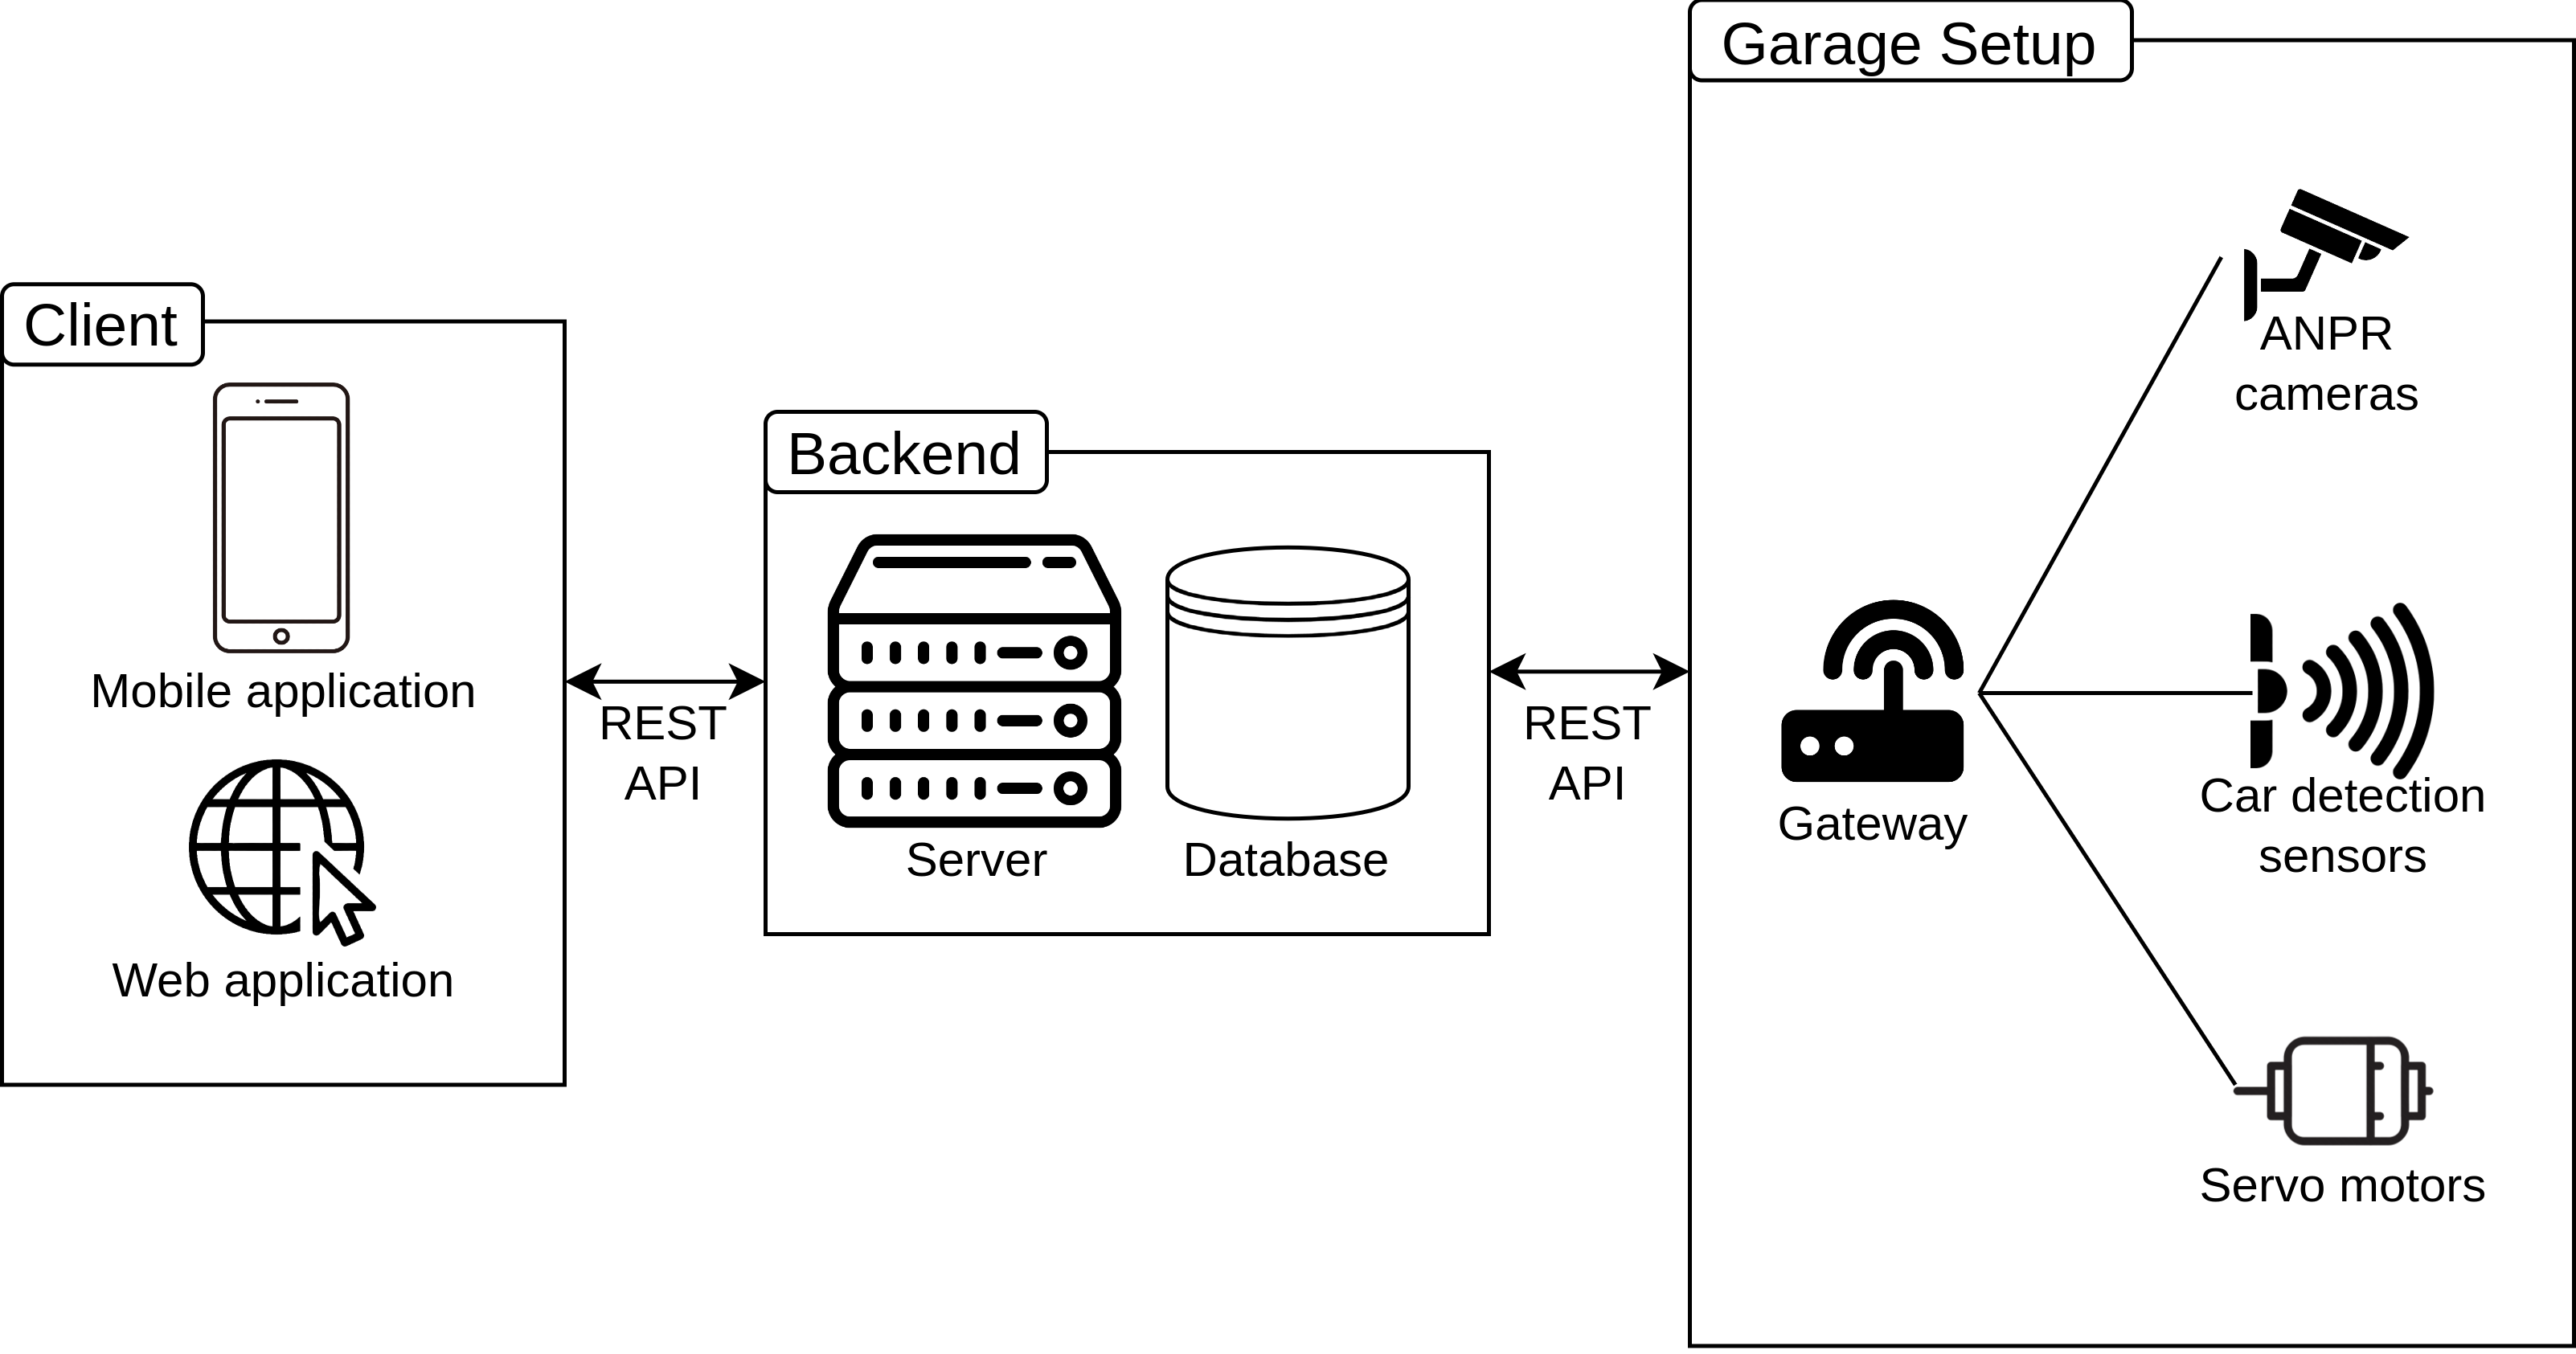
\includegraphics[width=12cm]{images/misc/abstract_diagram.drawio.png}
    \caption[Abstract overview of the intelligent parking system.]{Abstract overview of the intelligent parking system. The backend can be deployed on one psychical machine, which can run the proxy server and the database server in parallel.}
    \label{fig:abstract-diagram}
\end{figure}


\subsection{Core functionalities}\label{sec:core-functionalities}
The three main spearheads of the \ac{ips} described above are user privacy, security and ease of use. Table \ref{tab:core-functionalities} gives a summary of this paragraph, listing the three core functionalities, together with the steps taken to achieve them.
\ind Ease of use is split up in three sub-objectives.

\ind Firstly, it is not necessary for users of the parking garage to install the mobile application or even have a pre-existing account. It is possible for users to drive to the parking garage and park without any need for a prior setup, but receive an almost equal user experience.

\ind Secondly, if the user creates an account, he/she is able to reserve parking lots in a specific garage between specific times, in order to guarantee an available parking lot for the user at his/her arrival.

\ind Thirdly, the infrastructure supports automatic and non-automatic payments from within the frontend application, the former for users which created an account, the latter as an alternative for users without an account. 

\ind Besides the ease of use for the person parking in the garage, the frontend application also supports admin features for a garage owner. A garage owner can add or delete his/her garages from the system, as well as configure their parking lots. \\

Maximum user privacy is achieved by, firstly, not storing any information that is not needed for the operation of the \ac{ips} and secondly, hashing all user-identifiable and/or sensitive information (e.g. passwords, licence plates, email addresses) before it is stored inside the database. This way, even if an attacker obtains access to the database, he/she will not be able to retrieve any useful information from it.

\ind The two ways to park in the garage (i.e. with or without a pre-existing account) provide two levels of user privacy. If the user decides to park without an account, no user-identifiable information is stored in the database, except for the licence plate, which is deleted upon exit of the garage. This way, it is not possible to retrieve any personal information, nor information about the user's whereabouts from the system. From the standpoint of the system, that user ceases to exist upon exit of the garage. In the other case, licence plate information is coupled with the user's email address and a real first and last name, but history of the user's whereabouts are not stored (they are deleted upon exit of the garage).

\ind Making an automatic payment requires payment information from the user. This information is hashed before it is stored inside the database, but the user can opt for a manual payment, in which case no payment details are stored in the database.

\ind Furthermore, a garage owner is not able to query the users or licence plates in its garage, only the amount free parking lots left. \\ 

Security is the last core functionality. This mainly focuses on securing the backend, because it stores all important user information, but also includes securing the mobile application and the local garage setup, such that the sensors, nor the \ac{anpr}-cameras can be hijacked. 

\ind Firstly, the connections between the frontend and the backend and between the backend and the local garage gateway are encrypted. Secondly, the server only accepts traffic coming from the local garage gateway or the mobile application, which prevents \ac{csrf}-attacks. Thirdly, users can only query information regarding their own account (i.e. their personal information and bookings), which prevents \ac{idor}-attacks and fourthly, the \ac{api} can only be queried by authenticated users.

\begin{table}[htp]
    \centering
    \caption{An overview of the core functionalities of the entire system and how this is achieved on an abstract level.}
    \begin{tabular}{|>{\bfseries\centering\arraybackslash}m{1in}|>{\centering\arraybackslash}m{8cm}|}
         \hline
         \textbf{Core functionality} & \textbf{Achieved by}  \\
         \hline
         \hline
         Ease of use & \begin{itemize}[left=0pt]
             \item No obligatory account
             \item Reserving parking lots
             \item Automatic and non-automatic payments
             \item One application for both user and garage owners
         \end{itemize} \\
         \hline
         User privacy & \begin{itemize}[left=0pt]
             \item Least to know principle
             \item Hashing sensitive user information
         \end{itemize}\\
         \hline
         Security &\begin{itemize}[left=0pt]
             \item Encrypted connections
             \item Request origin validation
             \item Authenticated \ac{api}
         \end{itemize} \\
         \hline
    \end{tabular}
    \label{tab:core-functionalities}
\end{table}

\section{Implementation}\label{sec:implementation}
This section gives a detailed explication of the implementation of the core functionalities as described in Section \ref{sec:core-functionalities}. It is divided into four parts: Section \ref{sec:implementation-parking-garage} explains the physical model of the parking garage, Section \ref{sec:implementation-on-site-system} discusses the concrete implementation of the local garage system, Section \ref{sec:implementation-frontend} describes the different user flows within the frontend application and lastly Section \ref{sec:implementation-backend} outlines the backend system.


\subsection{Parking garage}\label{sec:implementation-parking-garage}
For the purpose of the  demonstration, a working model of the \ac{ips} was made. Since it is not in the scope of the project to create a full scale working parking garage, a scaled down model of a parking garage was created to show the functionalities of the \ac{ips}. The scale model meets the following set of requirements: 1) it has a sufficient amount of parking spaces to show the functionalities as described in Section \ref{sec:core-functionalities}; 2) it has working barriers to let cars enter and exit the parking garage and 3) it has signalling \acp{led} to show if a parking spot is occupied/reserved or available.

\subsubsection{Scale model}
The model has six parking lots that each have a cutout for a \ac{udms} which detect if a car is occupying a parking lot, as well as cutouts for the indication lights that will be green if the parking space is available and red if it is either occupied or reserved. There is a small entrance/exit road equipped with two barriers controlled by servo motors to stop cars from entering if there are no available spaces left, or to stop cars from exiting if they have not paid yet. Above the barrier is a horizontal beam that is used to mount the camera for taking images of the licence plates of the entering and exiting cars. On the entrance side of the road is a \ac{lcd} display mounted that shows the number of available spaces left in the garage. Underneath the parking spaces is an empty space that can be used to run the wiring and house the Raspberry Pi devices. Table \ref{tab:part_list} in Appendix \ref{app:part-list} shows an overview of all the used components in the local garage system.

\ind The scale model was laser cut out of \ac{mdf}-plates. All parts are secured together using press fit connections and further reinforced with hot glue. Figure \ref{fig:parking-garage} shows this scale model of the parking garage. 

\begin{figure}[H]
    \centering
    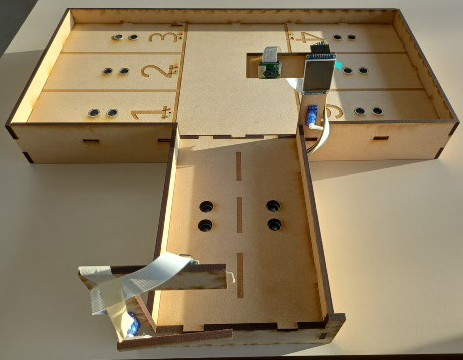
\includegraphics[width=10cm]{images/misc/parking_garage.jpg}
    \caption{Scale model of parking garage.}
    \label{fig:parking-garage}
\end{figure}

\subsection{Local garage system}\label{sec:implementation-on-site-system}
There are four main functionalities that the local system fulfils: 1) identifying cars by their licence plate, 2) detecting cars on parking spots and controlling the signalling \acp{led}, 3) operating the servo motors of the barriers and 4) controlling the \ac{lcd}-display. The backend server acts as a synchronisation for the multiple \ac{iot}-devices in the local garage system. In the current implementation, the local garages system uses two Raspberry Pi devices. Figure \ref{fig:deployment-garage-setup} shows the deployment diagram of the local garage system, with the different modules which run on the Raspberry Pi devices.\footnote{In this and the following paragraphs `Raspberry Pi' can be replaced by a more general \ac{iot}-device. The core principles remain the same.}

\subsubsection{Raspberry Pi}
The heart of the local system are two Raspberry Pi devices model B V1.2. They run a 64-bit \ac{os}\footnote{The amount of bits of an operation system is a characteristic of the processor and determines how many memory addresses the \ac{cpu} can access. \ac{cpu}s with 32-bit can access at most $2^{32}$ bytes ($= 4 \ \text{GB}$) of \ac{ram} \cite{bit-cpu}.}. This allows the usage of 64-bit Python packages, like \texttt{torch}\footnote{\url{https://pytorch.org/}}. The four main functionalities are separated into three Python packages\footnote{The code can be found in this GitHub repository: \url{https://github.com/orgs/2022PO3/repositories}.} which run in parallel. This provides a segmented approach to installing all the dependencies of the different packages. Furthermore, this makes it possible for the Raspberry Pi to run the multiple services together, making the overall system faster. Figure \ref{fig:general-deployment-diagram} in Appendix \ref{app:deployment-diagram} shows a schematic overview of the interaction between the software on the Raspberry Pi and the hardware components. 

\ind The first Raspberry Pi will also power and control the \ac{lcd}-screen. Moreover that, both Raspberry Pi devices take charge of one half of the parking garage (i.e. one camera, six \acp{led}, four \acp{udms} and one servo motor). The functionalities are subdivided into two main systems (and programs on the Raspberry Pi), namely the \verb|entrance_system|, which handles the entrance and exits of cards and the \verb|parking_lot_system|, which handles the detection of cars. The paragraphs below explain these systems more in depth.

\ind The Raspberry Pi communicates with the backend database with specifically designed \ac{api} endpoints (see Table \ref{tab:url-rpi} in Appendix \ref{app:backend-api-slugs} for more details about the specific \ac{api} endpoints) in order to update the different tables regarding the garages and parking lots. It also needs to be able to query the database, to –- for example –- receive information whether the user has paid or not. 


\begin{figure}[hpt]
    \centering
    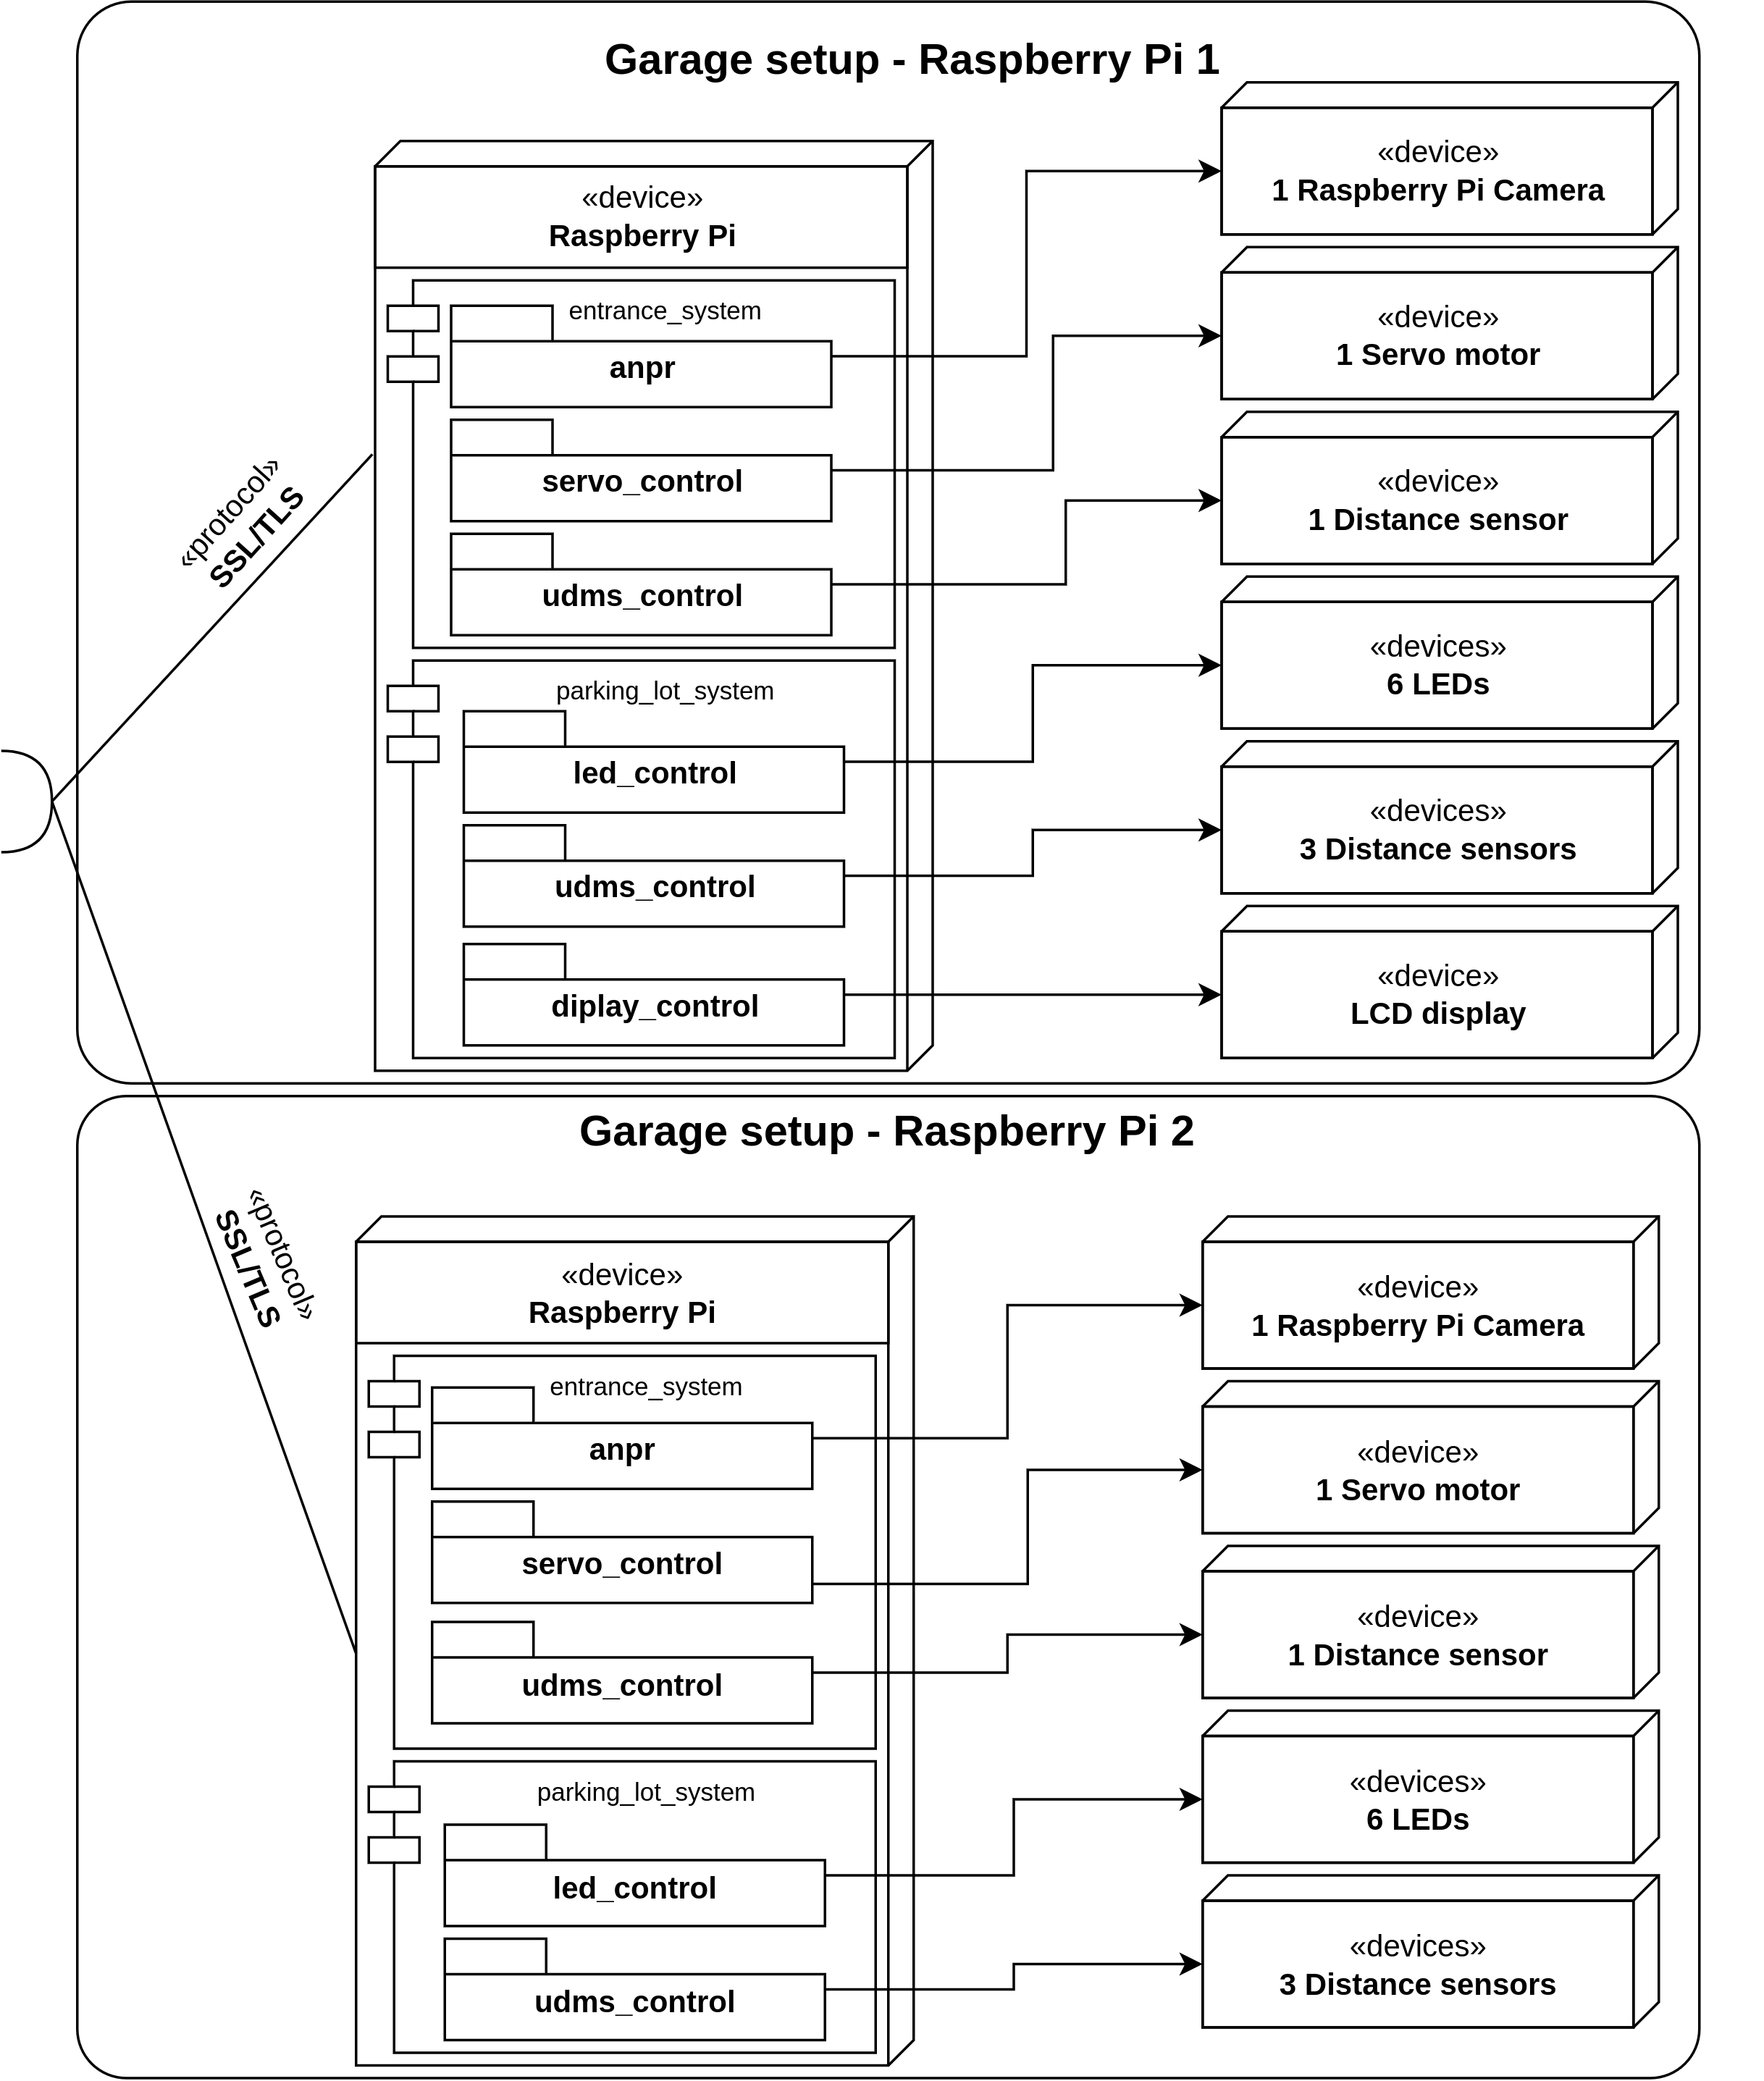
\includegraphics[width=10cm]{images/deployment_diagrams/deployment_diagram-rasperry_pi.drawio.png}
    \caption{Deployment diagram of the garage setup.}
    \label{fig:deployment-garage-setup}
\end{figure}

\paragraph{Entrance system}\label{sec:entrance-system}
The local garage system contains two cameras, both powered by a Raspberry Pi. Due to performance issues, the Raspberry Pi will only take a picture of the car and send the picture to the backend, which in turn executes the \ac{anpr} (see Section \ref{sec:anpr} fore more details). 

\ind The taking of the image is triggered by an \ac{udms}. The \verb|udms_control| remembers the previous state of the \ac{udms}. If the current state differs from the previous state, a picture is taken with a Bash script, to enhance speed. The image itself is sent to the backend. If the Raspberry Pi receive a positive status code (i.e \verb|200 OK|), \verb|servo_control| will open the barrier and close it after the car has passed. Automatically, the amount of free spots will drop by one in the backend due the successful posting of the licence plate image.

\ind The same procedure applies to the exit camera, but here the backend provides an additional check to confirm that the licence plate has paid. If not, the barrier will not open and the user will be notified in the frontend application that the payment has to be fulfilled before he/she can exit the garage. Automatically, the amount of free spots will increase by one in the backend due to the successful posting of the licence plate image.

\ind From the moment that the parking garage is completely full, either by physical cars or by reservations, the entrance system will refuse to enter new cars, except the ones with a valid reservation.

\ind Figure \ref{fig:sequence-diagram-licence-plate} in Appendix \ref{app:sequence-diagrams} visualises the entrance procedure in detail with a sequence diagram.

\paragraph{Parking lot system}
To know the amount of available parking places and to detect cars at the entrance or exit, the local system needs to be able to sense the presence of a car at a specific location in the garage. This can be done by several sensors. The most useful ones are \ac{udms} or light sensors. The latter is more expensive and does not offer any extra advantages over the \ac{udms}. For this purpose the demo garage uses the \ac{udms} (\textsc{hc-sr04}).

\ind The \ac{udms} can measure distance by sending ultrasonic sound waves. After the pulse bounces of an object, it gets detected by the same sensor. Using the time between sending and receiving the pulse, the distance can be calculated because the speed of sound is known. To reduce the risks of false positives, the Raspberry Pi remembers the last two states of every parking lot. From the moment that it detects a car (i.e. the distance measured is smaller than $5 \ \unit{cm}$) two consecutive times, a request is sent to the backend indicating that the parking lot is occupied and the red \ac{led} is turned on. The same procedure happens when a car leaves. 

\ind One Raspberry Pi has a second component to the \verb|parking_lot_system|, namely \verb|display_control|, which powers and controls the \ac{lcd}-display. This package will make a request to the backend every 5 seconds for the free parking lots left in the garage and display this amount (see Section \ref{sec:system analysis} for a discussion about this method).

\subsection{Frontend}\label{sec:implementation-frontend}
This section describes the implementation of the core functionalities of the frontend as described in Section \ref{sec:core-functionalities}. The frontend application is written in Dart, with the Flutter\footnote{\url{https://flutter.dev/}} framework of Google. Flutter is used, because of its platform independence (it can run both on Android, iOS and web), and its provided type safety and null safety. Furthermore, Flutter supports a hot reload feature, which makes it easy to develop the application. The next section gives a rough idea of how the app will work when it is launched. The application is subdivided into different pages. Each page is enumerated with a combination of letters and number; a new number indicating a new flow and a new letter indicating a new subflow. An overview and a short description of all app pages can be found in Appendix \ref{app:app-diagram}, Table \ref{tab:app-pages}.

\subsubsection{Application design}
The following paragraphs discuss the many functionalities of the frontend application. These functionalities are achieved using a multitude of screens, which are bundled into several flows in the application. Table \ref{tab:app-flows} gives an overview of all the major application flows and Figure \ref{fig:general-app-diagram} in Appendix \ref{app:app-diagram} gives a schematic overview of the relations between those screens. Of course, the routes defined in Figure \ref{fig:general-app-diagram} are the ideal routes, given that the user enters valid input, which is not always the case. The frontend application implements rigorous validation, such that all data entered will match the type and format asked by the backend. If the user enters non-valid information, he/she will not be able to continue and a dialog is displayed to the user containing the exact description of the errors. Figure \ref{fig:error-dialogs} in Appendix \ref{app:app-diagram} shows examples of this. Besides signalling errors, pop-ups are also frequently used to display information about the application or about the request the user has made. See Figure \ref{fig:information-dialogs} in Appendix \ref{app:app-pages} for examples of this.

\ind In general, if a button in the application is pressed which loads a new screen, a request is sent to the backend to get the information about the user, the garage or the reservation required to construct the page. When information has to be changed in the database, different requests are sent to the backend to post, change or delete information in the database. 

\ind The first page of the application is determined dynamically, based on the authentication state of user. If the user is both authenticated and verified (i.e. the user has logged in \textit{and} has provided a \ac{2fa}-code), the application will open the home page directly and the authentication flow will be skipped. If the user is unauthenticated, the login page is opened and the user has to follow the authentication flow. The third case exists when a user is authenticated, but not yet verified (and has \ac{2fa} enabled for his/her account). In that case, page 0c is opened for the user to submit their \ac{2fa}-code.

\ind The following paragraphs explain the flows more in depth. All referenced figures can be found in Appendix \ref{app:app-diagram}.

\paragraph{Authentication flow}
Depending on if the user is logged in or not, the login page is the first page the user lands on when opening the application. Here they will have the option to login with either their existing account or to register a new one. If they choose to make a new account, then the register page pops up. On this page users have to fill in their first name, last name, email address and password (a licence plate is later added, see Section \ref{sec:profile-flow}). These credentials are used to create a secure account. The user is required to confirm their password by entering the same password in another text field. This is required for lowering the chances of accidentally typing the wrong password. Once the necessary text fields are submitted, the user will be present in the database, but will not yet be active. An email is then sent to the given email address to verify that it is a real address. This email allows users to activate their account and subsequently log in.

\ind If the account is verified, the user can login by hitting the `Sign in'-button. When authenticated, the homepage will be loaded and the app will make a request to the backend server to load all the possible garages. Whilst the app is connecting with the backend, there will be a progress indicator on the screen and the user will still be able to access other features like the navigation bar (Pages 0, 0a, 0b and 0c; Figure \ref{fig:auth-flow}).

\paragraph{Home flow}
The home flow describes the options available to the user in the home screen itself. This includes opening the navigation bar, which provides the entry point for all major flows inside the application and checking the notifications (Pages 1, 1a and 1b; Figure \ref{fig:home-flow}).

\paragraph{Reservation flow}
The most important flow in the application is the reservation flow. After all the garages have been loaded into the app, the user can select one of the garages to make a reservation. Next the information screen will pop up of the selected garage. On this screen the user can observe the location, the amount spots left in the garage, the price and the opening hours. If the user is satisfied with this garage, he/she can book a reservation. There will be the option to choose a licence plate linked to the account (only enabled licence plates are able to make a reservation, see Section \ref{sec:licence-plate-validation}), the time and day of the reservation and an available spot in the garage. The user can choose between selecting a spot and getting a spot assigned at random. In the former, the app requests all available parking lots from the backend, out of which the user can choose one, in the latter, the backend returns a random free parking lot. Hereafter, an overview of the reservation is shown and the user is asked to confirm (Pages 2, 2a, 2b, 2c, 2d; Figure \ref{fig:user-reservation-flow}).

\paragraph{User settings flow}
The user settings flow is reached via the navigation bar in the home screen. The user can add a device in order to execute the \ac{2fa} and add credit card details for automatic payment. In addition, the \ac{2fa} and the automatic payment can be enabled or disabled as soon as a device or payment card is added. (Pages 3, 3a, 3b; Figure \ref{fig:user-settings-flow}).

\paragraph{User reservations flow}
This short flow enables users to view, alter and delete their made reservations. The current active reservation is highlighted in green; past reservations are greyed out. Note that it is possible for user with multiple validated licence plates to have multiple reservations at the same time. Multiple reservations on the same moment with the same licence plate are not allowed. See page 4 on Figure \ref{fig:user-reservation-flow} for more details.

\paragraph{Profile flow}\label{sec:profile-flow}
The profile flow is one of the more elaborate flows. When the user selects the ``Profile" tab in the navigation bar, two options are available: user information and licence plates. On the screen containing the user's info, he/she can change his/her first name, last name, email address and favourite garage name. To change their province or password another screen is shown and in order to delete your account a popup is shown. The favourite garage and the province can optionally be given by the user to enhance their experience as it alters the filtering of garage on the home screen (e.g. garages close to the user's location are displayed first) (Pages 5, 5d, 5d1, 5d2 and 5d3; Figure \ref{fig:profile-flow}).

\ind When the user selects the ``licence plates" button instead of the ``user information", there are several options. A licence plate can be added, which is shown on a popup on page 5a. If this plate already exists in the database and not under the current user's id -- meaning that it is possible someone else registered this licence plate with their account --, there is an option to report this. This to make sure that no one is able to follow the whereabouts of a person based on their licence plate. Furthermore, a licence plate can be enabled, as this is required in order to make a reservation for this vehicle. In order to do this, the vehicle registration document has to be uploaded, which is implemented in the application in order to further improve the user privacy. As this not a regular request to make, page 5b1 adds an explication why it is important to validate the licence plate before it is used (Pages 5a, 5a1, 5a2, 5b, 5b1 and 5c; Figure \ref{fig:profile-flow}).

\paragraph{Garage settings flow}
The garage settings flow is only accessible to users that have the role \verb+GARAGE_OWNER+. These users can see their garages in the navigation bar (Page 1a; Figure \ref{fig:home-flow}). They have the option to either configure their owned garages or they can add a new garage into the database. If the user presses on one of those garages, he/she will be redirected to a new page, where they can configure all the settings of the garage (Pages 6, 6a and 6b; Figure \ref{fig:garage-settings-flow}). 

\paragraph{Payment flow}
Payment is the last major functionality flow of the application. While actively being parked in a garage, a widget is present on the home page showing the licence plate of the vehicle parked and how long it has been parked for. When pressing pay on this widget, the user is able to see a receipt. When continuing, the user can pay for his park via Stripe on a browser tab inside of the app. Then the payment is either successful or unsuccessful. 
 In either way the user can return to the home screen. (Pages 7, 7a, 7a1 and 7a2; Figure \ref{fig:payment-flow}; see Section \ref{sec:Payment}) \\

For users who are not familiar using the app or a mobile app in general, there would be a guide in the navigation bar. However, this was not implemented in the final design due to a lack of time. Lastly, there is also an option to sign out the user's account. A detailed schematic overview of the entire app can be found in Appendix \ref{app:app-diagram} in Figure \ref{fig:general-app-diagram}.

\begin{table}[htp]
    \centering
    \begin{tabular}{|c|p{3cm}|p{10cm}|}
    \hline
         \textbf{Flow no.} & \textbf{Flow name} & \textbf{Short description} \\
         \hline
         \hline
         0 & Authentication flow & Flow for registering, logging in the user and sending the \ac{2fa}-code (Figure \ref{fig:auth-flow}). \\
         \hline
         1 & Home flow & Home page and banner which provides a step-stone for all major flows in the application (Figure \ref{fig:home-flow}).\\
         \hline 
         2 & Reservation flow & For making a reservation by selecting a licence plate, a spot and a date and time (Figure \ref{fig:reservation-flow}). \\
         \hline 
         3 & User settings flow & Flow for altering user settings like \ac{2fa} and enabling automatic payments (Figure \ref{fig:user-settings-flow}). \\
         \hline
         4 & User reservations flow & Screen for getting an overview of all user reservations (Figure \ref{fig:user-reservation-flow}). \\ 
         \hline
         5 & Profile flow & Flow for altering user information, e.g. name or password (Figure \ref{fig:profile-flow}). \\
         \hline 
         6 & Garage settings flow & Flow for garage owners which enables altering and adding of garages (Figure \ref{fig:garage-settings-flow}). \\ 
         \hline
         7 & Payment flow & Flow for making payments for parking (Figure \ref{fig:payment-flow}). \\
         \hline
    \end{tabular}
    \caption{Overview of the major app flows.}
    \label{tab:app-flows}
\end{table}

\subsubsection{Deployment}
The frontend deployment should support two use cases: users who want to download the mobile application and users who want to access the website.

\ind Due to Flutter's nature, it can run natively on all major platforms and operating systems. To make the mobile application accessible to the general public, it should be uploaded to the Google Play Store, the Apple App Store and the Microsoft Store. For the purpose of this project, the application will be installed on the devices of the team members.

\ind The web application should be hosted on a web server, for the users to be able to access the site. The backend already incorporates a web server, namely Nginx\footnote{\url{https://nginx.org/}}. Apart from being a reverse-proxy for the backend, it also hosts the static files (\ac{html} and \ac{js}). Figure \ref{fig:deployment-frontend} shows the deployment diagram for the frontend application. Note that the two client devices represent both options of the client connection to the backend \ac{api}.


\subsubsection{Backend communication}
The frontend needs communication with the backend in order to show the user the right information. This is achieved by using a \ac{rest} \ac{api}, which exposes different \acp{url} to the client. Tables \ref{tab:general-url}, \ref{tab:auth-url} and \ref{tab:url-payment} in Appendix \ref{app:backend-api-slugs} provide a detailed overview of all the different \ac{api} endpoints exposed by the backend. When the client sends a request to one of these \acp{url} an action happens in the backend based on the request. There are four different types of requests implemented in the backend: \verb|GET|, \verb|POST|, \verb|PUT| and \verb|DELETE|. These requests respectively receive, post, change and delete information.

\begin{figure}[H]
    \centering
    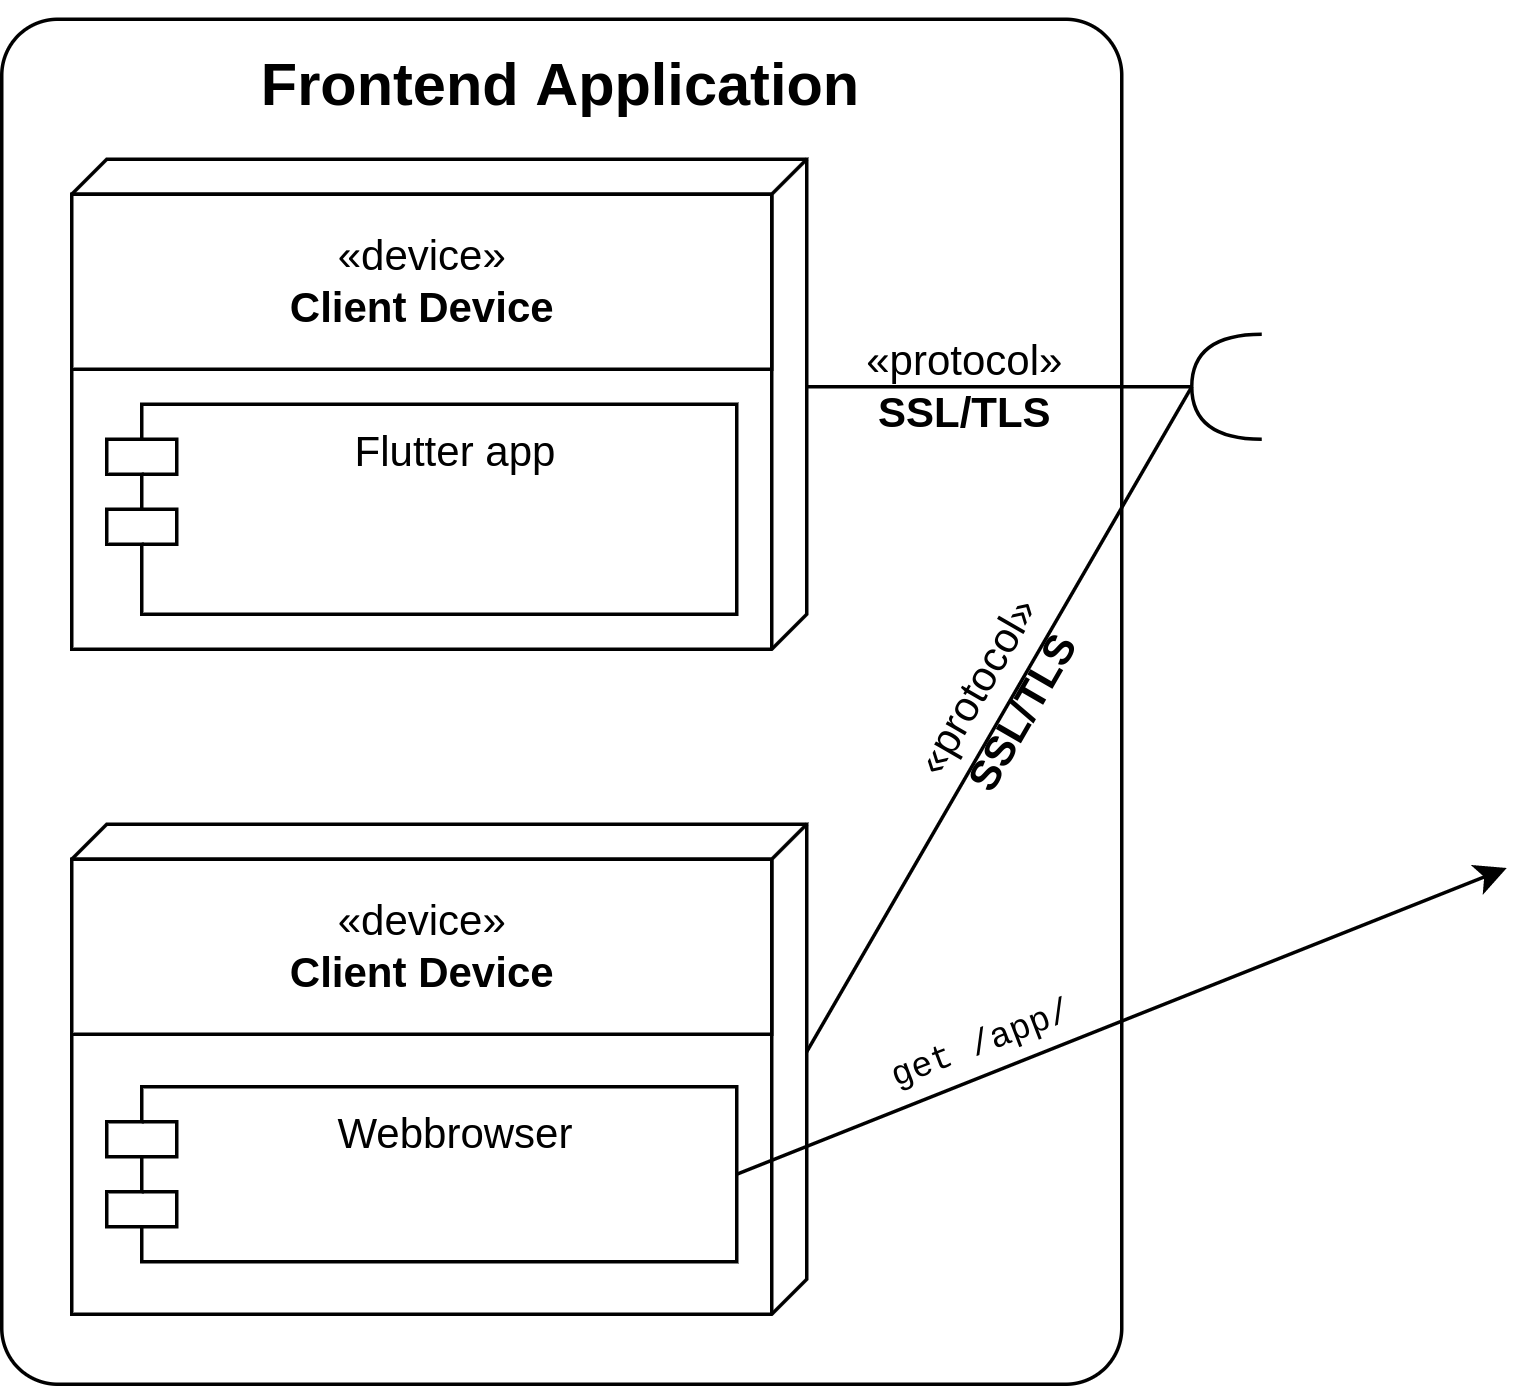
\includegraphics[width=8cm]{images/deployment_diagrams/deployment_diagram-frontend.drawio.png}
    \caption{Deployment diagram of the frontend application.}
    \label{fig:deployment-frontend}
\end{figure}

\ind To further explain this communication, the creation of a reservation is a good example. As soon as a user selects a garage, an overview of this garage is given. In order to show this page, a \verb|GET| request is first sent to the \ac{url} of the garage, specified using the index of the garage (\verb|/api/garage/<int:pk>|). This request receives all the information of the garage needed to construct the page shown. Later on, when the user has selected a time and date, in order to select a spot another request is sent to the backend. This time also a \verb|GET| request, sent to the \ac{url} concerning the parking lots of a certain garage (\verb|/api/parking-lots/<int:pk>|). A list of parking lots is returned, with their respective state and information. Based on this list, the frontend can build the page for spot selection. After the overview of the reservation, when the user confirms, a \verb|POST| request is sent. This request arrives at the \ac{url} concerning the reservations of the user (\verb|api/reservations|) and a reservation is added to the database. Figure \ref{fig:sequence-diagram-reservation} in Appendix \ref{app:sequence-diagrams} gives a schematic overview of the different requests made with a sequence diagram.

\ind The above requests are just examples of the many requests sent to the backend in the usage of the frontend. Since the latter is not functional without these requests, the communication between front- and backend is very important for the system.

\subsection{Backend}\label{sec:implementation-backend}
The main functionalities of the backend are described in Section \ref{sec:core-functionalities}. This section describes the implementation of those core functionalities. Section \ref{sec:design-motivation} outlines the augments for the different software used in the backend.

\ind The main parts of the backend described below can run on a single physical machine. The deployment of those services can happen both on a local server or on a cloud server. For the purpose of this project, a local home server is preferred, but a real-world system requires scalability which makes a cloud server indispensable.

\subsubsection{Server}
The server is the main entry point to the outside world of the database and the \ac{rest} \ac{api} and thus needs proper security measures. The encryption of traffic happens on the server, origin validation to prevent \ac{csrf}-attacks is included in the backend application (see Section \ref{sec:backend-application}). 

\ind Nginx is used as the main \ac{http}-server in the backend. It serves as an industry standard for a fast and lightweight server. The most important feature for the backend is that it can handle \ac{ssl}/\ac{tls} and redirect \ac{http}-requests to \ac{https}-requests \cite{nginx}. Furthermore, the server has to redirect incoming requests to the right application, namely, the web variant of the frontend application or the backend application. This is achieved via a \textit{proxy-pass}, which can redirect traffic from one server to another, based on certain conditions in the request (e.g. all \acp{url} which starts with \texttt{api/} are redirected to the Gunicorn Python server (see below).

\ind Besides a web server, the backend application needs a way to communicate between the web server and the actual application (in casu the Django application). This is achieved with a \ac{wsgi}. The backend uses Gunicorn\footnote{\url{https://gunicorn.org/}} as its \ac{wsgi}. The main purpose of the \ac{wsgi} is making the deployment more stable and faster. The former is achieved by running multiple instances of the Django application, which improves the overall availability of the system \cite{gunicorn}. Besides improving the deploy stability, the \ac{wsgi} makes it possible to use a Nginx server as reverse proxy for redirecting \ac{http} to \ac{https}-traffic. This is not possible without a \ac{wsgi}.

\ind The services above require a lot of dependencies and configuration files, which can make it tedious to set up on a remote machine. The backend is therefore deployed with Docker containers, which bundles \textit{Docker images} with an \ac{os} in a so-called isolated \textit{container}. In this way, all the dependencies are packed inside the container, which eliminates the need of doing a laborious setup on the server machine. In total, there are three containers, one for the Nginx server, one for the Gunicorn gateway which runs the Django application and one for the MySQL database. The containers run as a single service with Docker Compose, which makes communication between the different containers effortless \cite{docker-compose}. Figure \ref{fig:deployment-backend} shows the deployment diagram of the entire backend.

\begin{figure}[htp]
    \centering
    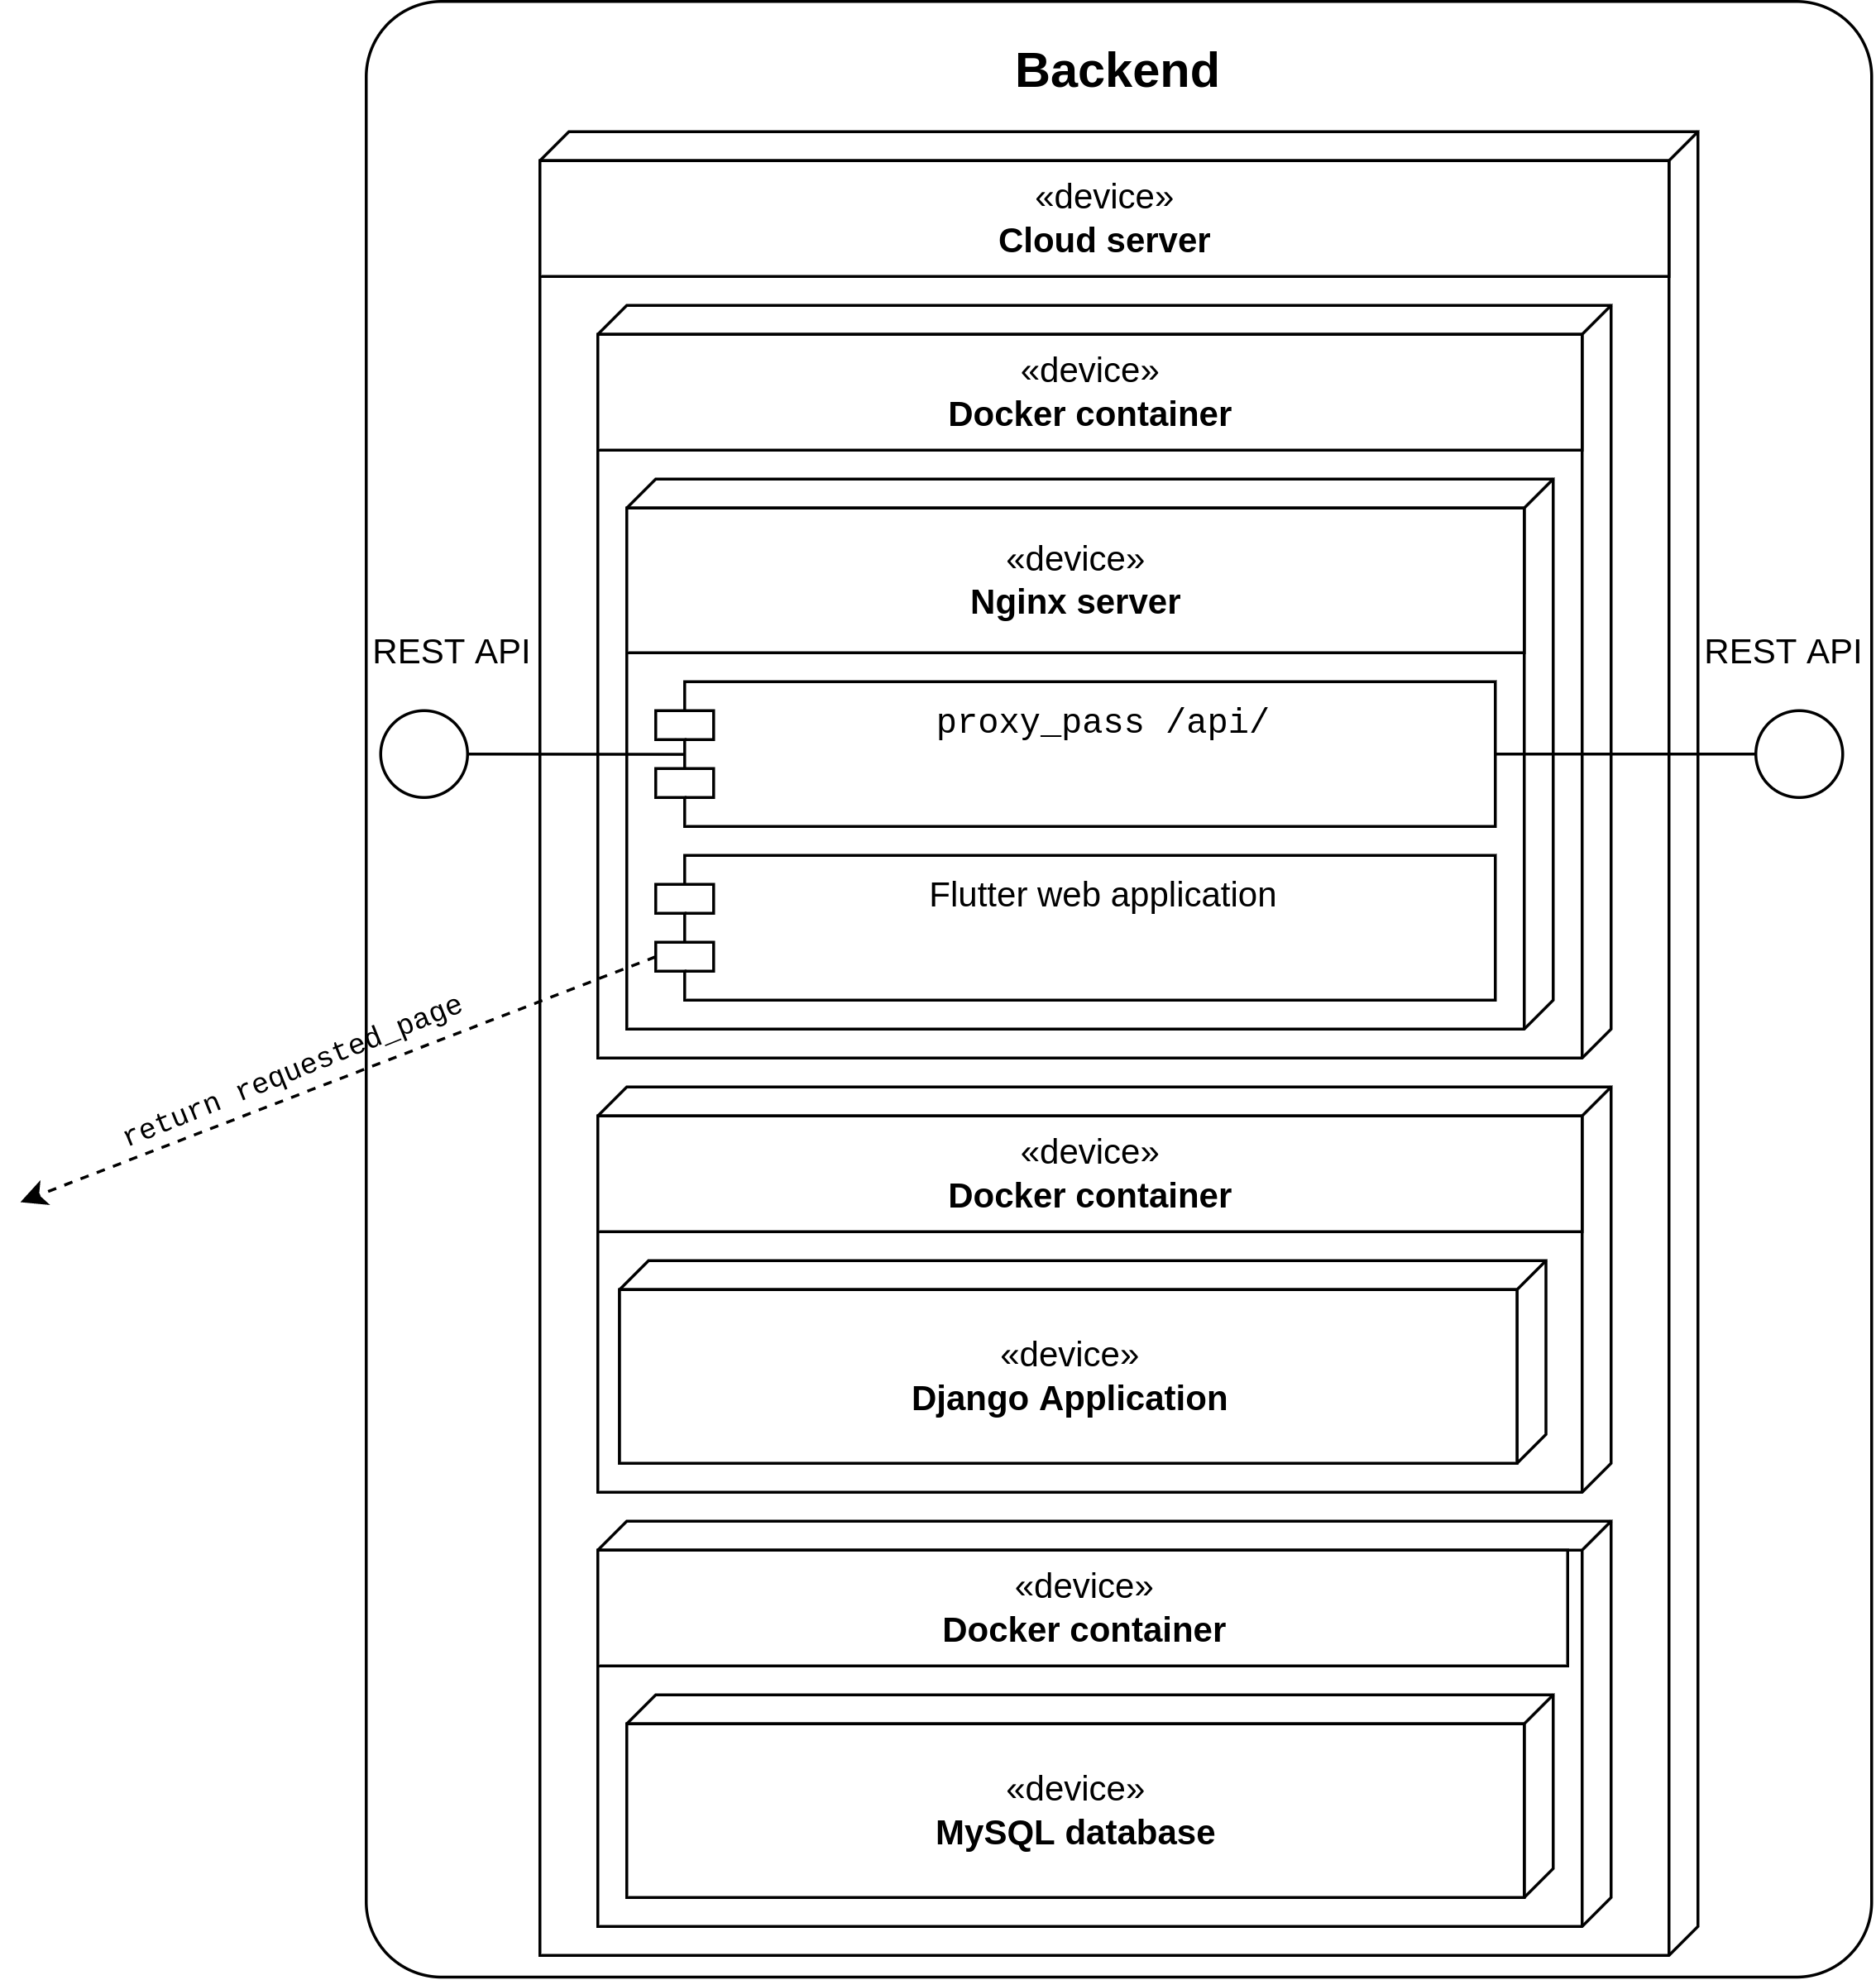
\includegraphics[width=8cm]{images/deployment_diagrams/deployment_diagram-backend.drawio.png}
    \caption{Deployment diagram of the backend server software.}
    \label{fig:deployment-backend}
\end{figure}


\subsubsection{Backend application}\label{sec:backend-application}
The backend server-side application is written in the Django framework. The Django framework serves as an \ac{orm} for the database, which makes it much easier to query the database. The main purposes of the backend application is to retrieve the right information from the database and more importantly, validate if the user is authenticated and authorised to query that information. The database itself is a MySQL, relational database.\footnote{\url{https://www.mysql.com/}} 


\paragraph{User authentication}\label{sec:user-authentication}
User authentication is an essential part of the \ac{ips} in general, due to the fact that this is the primary defence against unauthorised querying of the \ac{api}. The authentication system in the backend consists out of three \textit{views}: registering a new user, logging in a user and logging out an existing user. 

\ind In general, there are three levels of authentication for a user in the backend: \textit{unauthenticated}, \textit{authenticated} and \textit{authenticated and verified}. When a user is not logged is, it is called unauthenticated. If the user has \ac{2fa} enabled and has logged in (meaning an authentication token exists in the database, see further), but has not yet entered their \ac{2fa}-code, it is authenticated, but not yet verified and thus not able to perform any requests. Only if the user has both authenticated and has verified its \ac{2fa}-code it is able to perform requests.

\ind If the user creates a new account with the frontend application, their record will be added to the \texttt{users}-table, but this account is not yet functional. Upon registration an email is sent to the user with an activation link. Once the user has clicked on this link, their account will be activated and can be used to log in.

\ind A user can log in via the frontend application which sends the entered \texttt{email} and \texttt{password} to the backend via an encrypted \ac{ssl}/\ac{tls}-connection. The backend validates the credentials and if they are correct, an \textit{authentication token} is generated and sent back to the frontend. This token has to be used in \textit{all} \ac{api}-requests which query or pass data from and to the database. Furthermore, this token indicates if a user is logged in or not. If a token is present in the \verb|knox_authtoken|-table, a user is considered logged in. To prevent attackers from logging in with this token from a separate device, the number of tokens is limited to one token per user. If someone tries to log in with the credentials of an already logged in user, an error is returned. This token also makes it possible for the frontend to implement an automatic login system for the users.

\ind From the frontend application, users are able to log themselves out. From a backend's perspective, this means deleting the authentication token from the database. In order for the logout to succeed, the authentication token has to be sent with the request. This prevents unauthorised logging out of users. 

\paragraph{Serialization of database models}\label{sec:backend-serialization}
All data is transmitted in \ac{json}-format in the \ac{api}, but it cannot be directly inserted in this format in the database. One of the tasks of the backend application is \textit{serializing} the data between the \ac{json}- and database formats. This not only happens when data is queried from the database, but also when data is posted to the \ac{api}. In this direction, the serializing function becomes more important, because it \textit{validates} the sent data. The data has to match the requirements of the schema of the database (e.g. certain columns of the database are non-null, others have to be unique, etc.). If not, an error message is returned to the sender and the record will not be stored. This procedure is also the main defence against \ac{sql}-injection.

\ind On the backend level, models are related to each other, which makes it possible to build complex data structures. Possible relations are \verb|has_many| or \verb|has_one|, which indicates that a parent model can have multiple or only one child model, respectively. Figure \ref{fig:class_diagram} shows a schematic overview of these relations. 

\begin{figure}
    \centering
    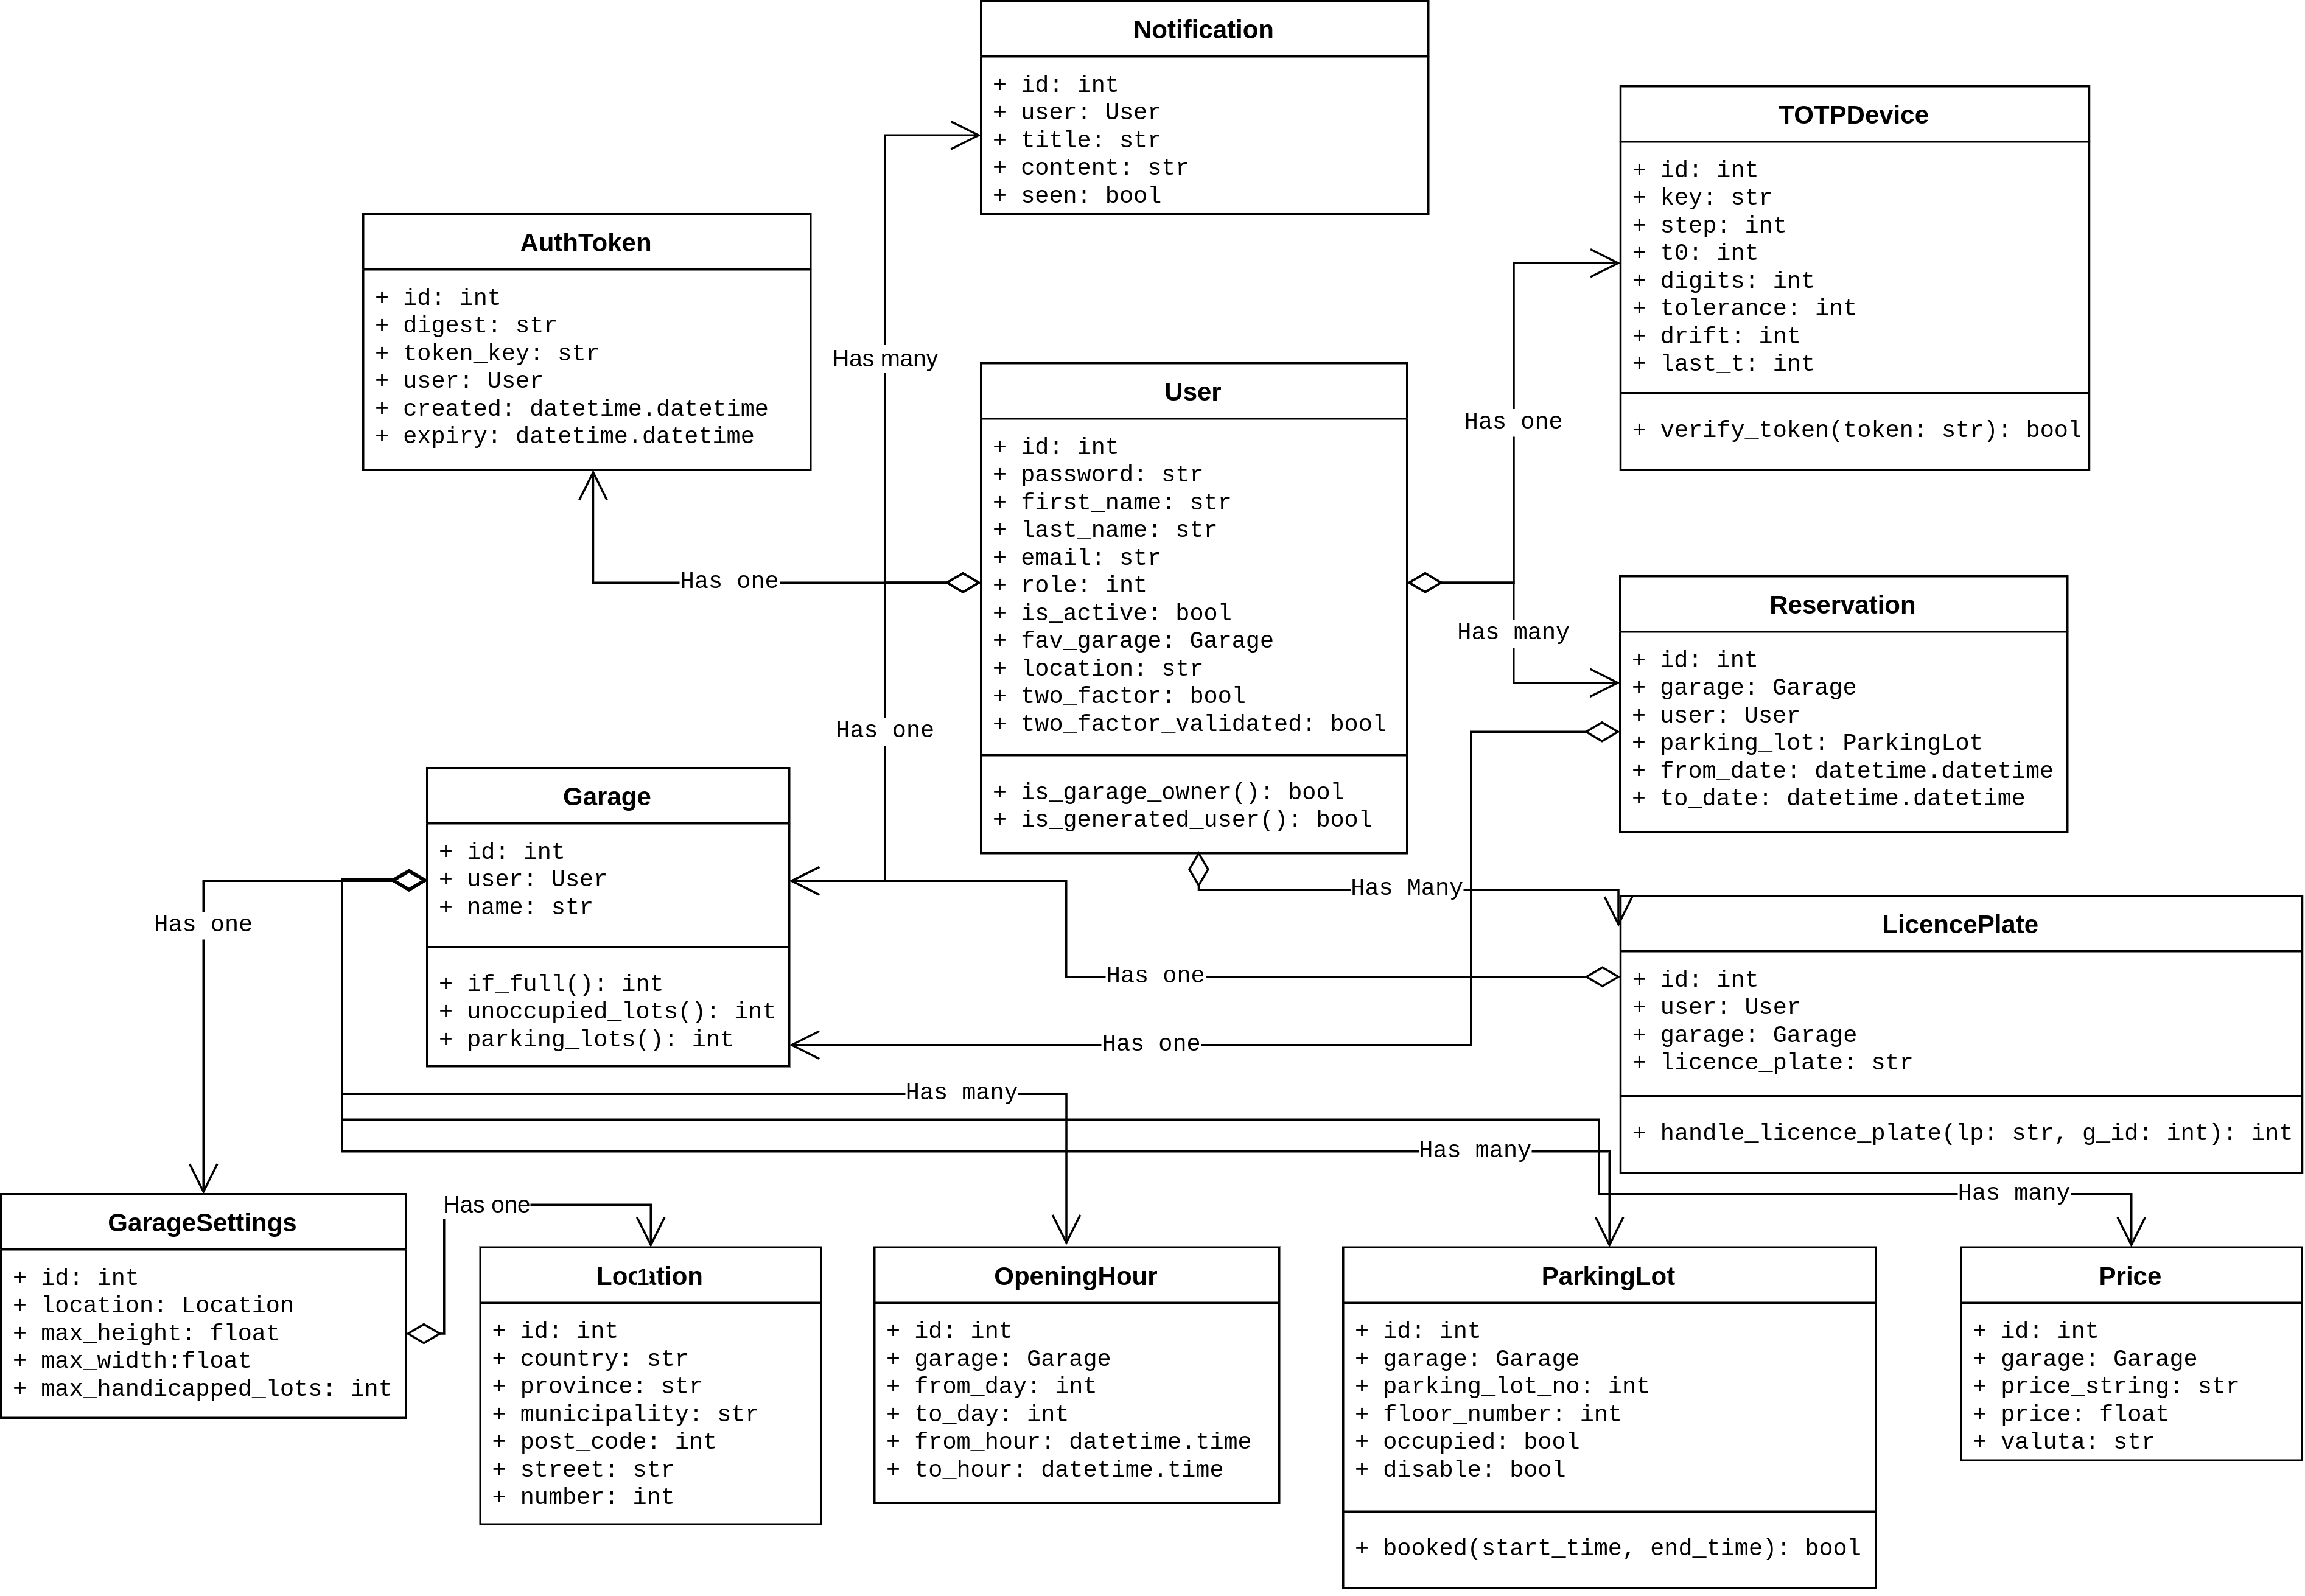
\includegraphics[width=14cm]{images/misc/class_diagram.drawio.png}
    \caption[Class diagram of the backend.]{Class diagram of the backend, which shows the relations between the different models. Note that the relations are only marked one-way, while they exist both ways in practice.}
    \label{fig:class_diagram}
\end{figure}

\paragraph{User roles}\label{sec:backend-roles}
All users in the database have one specific role, which is associated with a set of \textit{permissions} for this user. There are three roles: \verb|GENERATED_USER|, \verb|NORMAL_USER| and \verb|GARAGE_OWNER|. Upon registration with the frontend application, the default role is \verb|NORMAL_USER|. In order for a user to register as a \verb|GARAGE_OWNER|, the user has to provide the necessary legal documents which proves its ownership of a garage. The set of permissions of the \verb|GARAGE_OWNER| is a superset of the user permission set, with the added permissions of adding and deleting garages and adding, disabling and deleting parking lots.

\ind The \verb|GENERATED_USER| is a special role which is created upon entering of a user without an account in the parking garage. The \ac{anpr}-cameras send registered text of the licence plate to the backend. Then the backend checks if the licence plate is already registered in the database. If not, a new dummy user, with the role \verb|GENERATED_USER| is created with the associated licence plate. This account only serves as a visualisation of the parameters of the user's park (e.g. duration) and has no functionalities which are found in a normal user's account. Upon exiting the garage, the backend checks the associated role of the user; if it is a \verb|GENERATED_USER|, the account -- with the associated licence plate -- is deleted.

\ind A user can also be banned from using the system, setting its \texttt{role}-attribute to inactive. When a user does not show up at a reservation for a third time, its account will subsequently be banned. With each no-show, a notification in the application will notify the user about the imminent banning of its account.

\paragraph{Automatic number plate recognition}\label{sec:anpr}
The backend implements \ac{anpr} to identify cars coming in and out of the garage. It is performed on the image which is sent to the backend via the Raspberry Pi (see Section \ref{sec:entrance-system}). Its goal is to reliably detect the licence plate from different angles, light conditions and quality of the image. There are multiple ways to solve this problem. It is possible to use machine learning, however this requires a large dataset of good quality images to train the model. Creating these datasets takes a lot of resources, so this approach is out of the scope for this project. Another way to detect the text on the licence plates is to firstly find the licence plate on the image and then read the text in the region of the licence plate \cite{anpr}. The advantage is that there are already publicly available \ac{ocr} tools to find text in images. 

\ind The licence plates can be located because of their predictable shape. They are rectangular with a certain range of possible aspect ratios and have mostly contrasting colours. For this purpose, an algorithm can find candidates of licence plates by converting the image to greyscale and applying a threshold to it. The image now only has black and white pixels, indicating the dark and light regions. In these pixels it can then look for rectangular regions. Out of these candidates, the algorithm can select the real licence plate based of the (amount of) text on it. It can also filter them based on given licence plate formats. In Belgium, for example, most licence plates have the `1-ABC-123' format. The filters can be changed easily because it is an argument to the OCR-function. This approach will not work in real applications because of unknown formats or custom licence plates but this approach is sufficient for this project.

\ind To read the text on the licence plates, two \ac{ocr} tools are used: EasyOCR \cite{easyocr} and Google Vision \ac{api} \cite{googlevision}. EasyOCR is free but less accurate, this is perfect for filtering out the licence plate candidates without any text on it. Google Vision \ac{api} is a paid service, it costs \$1.5 for 1000 requests with 1000 free requests per month, but it is almost error-free. Google Vision is only used on the final candidate to stay below these 1000 requests.

\paragraph{Payment}\label{sec:Payment}
The backend supports two main payment options: manual payments and automatic payments. For the manual payments, users can use all mainstream payment methods (e.g. Bancontact, iDeal), for automatic payments only card payments are supported. All payments are handled by the Stripe platform.\footnote{\url{https://stripe.com}} They provide simple integration of more payment methods, as well as an easy to use dashboard to get an overview of all payments. This project uses their checkout (manual payments) and invoice (automatic payments) \acp{api}. 

\ind When a user wants to pay, the backend has to know how much it should charge, regardless of the payment method. It calculates the required amount based on the prices of the garage stored in the database and the duration for which a user is parked. The garage can have multiple prices, each based on a different parking duration. To get the best price the algorithm starts with the price with the longest duration and subtracts it from the parking time as much as possible, then the same thing happens for the next price and so on. For example, when there are prices for 1 day, 8 hours and 1 hour present in the database, and the user parked for 12 hours, they have to pay the price for 8 hours once and the price for 1 hour four times. The cumulative amount is then charged to the user.

\ind The manual checkout can be used by all users. When a request for manual payment is sent to the backend, it sends all the prices and their quantities (as explained above) to Stripe. Stripe subsequently creates a checkout \ac{url}, which is then returned by the backend as well. Finally, the frontend redirects the user the checkout page using the requested \ac{url}. Figure \ref{fig:manual-payment} in Appendix \ref{app:sequence-diagrams} visualises this schematically with a sequence diagram.

\ind To use automatic payments, a user has to add a card to their account. This can be done by sending the necessary details (card number, expiration date and \ac{cvc} code) to the backend.\footnote{Note that the backend \textit{does not} store these credentials. They are only needed to create a customer at Stripe, where after they are deleted from the backend systems.} After that, a new customer is created on Stripe, this is necessary for storing the new card payment method. When a user with a connected card tries to leave the garage, the backend can automatically charge the card using the invoice \ac{api} and the customer on Stripe. Figure \ref{fig:automatic-payment} in Appendix \ref{app:sequence-diagrams} displays this process schematically with a sequence diagram.

\ind The backend can detect succeeded or failed payment attempts using \textit{webhooks}.\footnote{Webhooks are functions which can be called based on certain events happening on the web page, e.g. a user making a payment.} This means that \textit{Stripe} will make a request to the backend \ac{api} for each new event. When the payment was successful, the licence plate of the user is updated so that it can leave the garage. If the payment failed, the backend sends an email to the user with a new payment \ac{url}.

\ind The frontend application also allows garage owners to make an account with Stripe and so receive the payments from the users who paid in the garage. 


\subsubsection{Security}\label{subsec:sucurity}
As explained in Section \ref{sec:core-functionalities} security is one of the most important aspects of the backend. Of course, security is not limited to the backend alone, as it is often a conjunction between the frontend and the backend

There are numerous attacks possible against a backend service, so it is not possible to list them all. The following sections will describe the most common vulnerabilities and how they are prevented. Table \ref{tab:backend-security} gives a schematic overview of the following paragraphs.

\paragraph{Injections attacks}
Generally, during an injection attack, an attacker will try to inject malicious input in the backend system, most often done via the frontend application, which allows user to input data \cite{injection_attacks}. The most common types are \ac{xss}, in which the attacker tries to input (most-often \ac{js}) code into the remote server and \ac{sql} injection, in which the attacker tries to input \ac{sql}-commands into the server.\footnote{Note that there are many more possible injection attacks, like buffer overflows, format string attacks and command injection, etc.} If any of these succeed, it can lead to the \ac{rce}, which makes the server vulnerable for leaking sensitive information or to redirect users to the malicious sites. Depending on the severity, an attacker is able to perform any command on the server. The primary defence  against injection attacks is the sanitising of user input.\footnote{Note the difference between \textit{serializing} (see Section \ref{sec:backend-serialization}) and \textit{sanitising} data.  The former is needed for compatibility between the frontend and the backend, the latter is an essential tool for preventing injection attacks.} This includes escaping any non-alphabetic characters. A second key point is setting a max-length on \textit{all} input fields, in which the user can enter data. This specifically prevents database corruption through memory corruption. The use of Docker container, provides an isolated environment for the backend to run in. This reduces the risk of command injection attacks.

\paragraph{\acp{acm}}
From a backend's perspective, there are three \acp{acl}, associated with the roles, described in Section \ref{sec:backend-roles}. Each \ac{acl} has a strict associated set of permissions, which prevents that users perform actions which they should not perform (e.g. altering information about a garage) and that users cannot alter objects, on which they have no ownership (e.g. altering information about a different user). The backend is designed in such a way that requests that the user parameter is determined automatically from the authentication token, without sending it directly with the request. This prevents \ac{idor} and the malicious editing of objects. 

\ind Apart from determining the user automatically from the request, the backend implements an additional set of permissions to the role \verb+GARAGE_OWNER+. They are allowed to add garages and parking lots to the system, as well as to alter or delete garage and parking lots which they own.


\paragraph{Request Forgeries}
\ac{csrf}-attacks and \ac{ssrf}-attacks are different but related attacks, which are caused by a lack of origin validation with the server. In the former, an attacker misuses the user credentials to perform actions as if the attacker was the user, in the latter the attacker targets services which are running internally on the server, causing it to leak sensitive information.

\ind The backend implements a rigorous origin-validation system, with the use of \ac{jwt}-tokens.\footnote{\url{https://jwt.io}}\textsuperscript{,}\footnote{Note that this token is different from the authentication token which is used for authentication the uesr.} Each time a request is made, the frontend application will generate a new \ac{jwt}-token. It is signed with a secret key only known to the backend server and the frontend application. The \ac{jwt}-token only lives for 5 seconds, preventing the capture and reuse of these tokens. 

\ind Based on the deployment diagram, the backend has to be able to accept requests from two different origins: the local garage system and the frontend application. All requests from any other location are rejected. This prevents both types of attacks mentioned above: if the attacker gets hold of the user's authentication token, he/she will not be able to perform any requests with it, as only the frontend application can send valid requests to the backend server. Furthermore, an attacker will not be able to gain access to internal services running on the server as it is only accessible via the frontend application, which can only interact with the Django framework.

\ind The origin-validation of local garage system proceeds in a similar fashion, but the \ac{jwt}-token has no expiry, as it cannot be intercepted as the data is sent via \ac{https} and thus the sent data as well as the cookies are encrypted. This further prevents \ac{mitm}-attacks.

\paragraph{Other security measures}
Apart from the above measures taken to enhance security of the backend, the backend also obliges users to choose strong passwords\footnote{The backend demands that a password is at least 10 characters long, contains a capital letter, a numerical symbol and a special character and may not be associated with any user information.} and allows the use of \ac{2fa}. Once the user is logged in, he/she can add a \ac{totp}-device. The backend then returns a security code which the user can enter in \ac{tpa} like Google Authenticator.\footnote{\url{https://play.google.com/store/apps/details?id=com.google.android.apps.authenticator2&gl=US}} From then on the user has to be both authenticated and verified to perform any requests. 

\ind The backend also requires the users to validate their email address given at sign up. If the user signs up, their object will be added to the database, but it will be inactive. Users will not be able to log in until they activate their account. This limits the creation of accounts with false email addresses.

\begin{table}[htp!]
    \centering
    \begin{tabular}{|c|c|}
         \hline
         \textbf{Attack}& \textbf{How prevented?}  \\
         \hline
         \hline
         \ac{sql} injection & Serializing all user input. \\
         \hline
         \ac{xss} & Serializing all user input (also in the frontend application).\\
         \hline
         \ac{idor} & User data requests return only info about the current user. \\
         \hline
         \ac{acm} & Strict \acp{acl} with added permissions. \\
         \hline
         \ac{csrf} & Use of a strict origin validation policy with \ac{jwt}-tokens. \\
         \hline
         \ac{ssrf} & Use of a strict origin validation policy with \ac{jwt}-tokens. \\
         \hline
         \ac{mitm} & Use of \ac{https}. \\
         \hline
         Brute force & Rigorous password policy \\
         \hline
         Stolen password & Possibility of \ac{2fa}. \\ 
         \hline
    \end{tabular}
    \caption{Overview of the backend's security measures against different attacks.}
    \label{tab:backend-security}
\end{table}


\subsubsection{Privacy}
Besides security, privacy is another core functionality of the \ac{ips}. As the backend is responsible for storing sensitive information about the user, it is most suited to build a solid privacy policy.

\paragraph{Least to know principle}
The backend implements the so-called `least to know principle`, which indicates that it only stores the information it actually needs to function properly. All other data is either not stored in the backend data (e.g. credit card details of the user) or deleted from the moment the data becomes irrelevant (e.g. information about a user's reservation is deleted two hours after the reservation is finished). Even in the event of a data breach, no relevant information about a user can be obtained. Other sensitive information, like passwords are hashed before they are stored in the database.

\paragraph{Licence plate validation}\label{sec:licence-plate-validation}
Some current parking applications make it possible for people to be followed based upon their licence plate \cite{privacy_breach}. This is a major privacy breach. In the frontend application, users can add a licence plate to their account, but it is not activated (and cannot be used to make reservations) until they submit a valid vehicle registration document proving the ownership of their licence plate. Furthermore, the \verb|licence_plate|-column has to be unique, meaning that it is impossible for different users to add the same licence plate to their account. The frontend application provides an additional possibility to report a licence plate if a user thinks that someone else has registered their licence plate.

\paragraph{Anonymous use}
The backend also fully supports anonymous use of the \ac{ips}, without giving in to user-friendliness. 
It is possible that a user drives towards a garage, without having the account and without having the application installed and yet have a similar parking experience to users with an account and in complete anonymity. In the case described before, the backend will generate a user with the associated detected licence plate. The local garage system will print out a paper ticket with a \ac{qr}-code on it. Scanning this \ac{qr}-code opens the frontend application, hosted on the Nginx-server, with the user already logged in with the generated account. This account allows the user to see in which garage they are parked, the time they are parked and a way to pay the due amount. Upon exiting of the garage, this account, with the associated licence plate will be fully deleted from the database. From a backend's perspective, the park ceases to exist to moment the user exits the garage, which renders it untraceable.
\section{Design motivation}\label{sec:design-motivation}
The design discussed in this report was not chosen without careful consideration of all options. The first decision made, was which micro controller to use. Common types of micro controllers such as a Raspberry Pi or an Arduino are readily available and are suitable for the project's needs. The Raspberry Pi 3B was used because the department had it available. \\

Secondly, the detection of entering or leaving cars can be done by cameras with motion detection software. This means that the camera is constantly running and detects whether or not there is any movement. The positive side of this method is that there is no need for any sensors or other extra hardware. The downside is that it might be too much to handle for the Raspberry Pi. An alternative option is working with sensors (e.g. a distance sensor) to detect the cars. This is less heavy for the Raspberry Pi, but adds an extra cost to the garage. Another option would be to leave the cameras filming and run the algorithm directly on the video footage. But this may also be too much to handle for the Raspberry Pi. Therefore, the option with the sensors is chosen for this project. \\

Thirdly, the detection of available parking spaces can be done by several sensors. The most useful ones are \ac{udms} or light sensors. The latter is more expensive and does not offer any extra advantages over the \ac{udms}. For this purpose the \acp{udms} (\textsc{hc-sr04}) are used in this project.\\

Fourthly, The backend application is written in Django, an open-source web framework, written in Python. The eventual decision was made based on the following concerns: 1) Python is known to all group members; 2) Django is a very explicit framework, which does not include a lot of magic features like Ruby on Rails does; 3) Django describes itself as the ``framework for perfectionists with deadlines'', which is exactly suited for the job \cite{django_website}. \\

Lastly, the frontend application will be written in Dart, with the Flutter framework of Google. Other valid alternatives were primarily JavaScript (\ac{js})-frameworks (e.g. React or AngularJS). The main benefit for Flutter
over the other frameworks is that it can run on any operation system (Android, iOS, MacOS, Linux, Windows,
etc.), that it provides type safety and null safety (Dart is a strongly typed language) and that it supports
hot reloads, which makes development much easier [Flutter, 2022]. Furthermore, two of the team members
already worked with Flutter. \\

Of course the price of the different components played also a big part in the decision making. The prices of the individual components and the total price can be found in Table \ref{tab:budget}. The leftmost column gives the name of the component used in the
model. The second column shows how many pieces of that component are needed. Column 3 shows the price per piece and column 4 the total price for a specific component.
The budget for this project is 250 euros. The design uses a total of 224.87 euros, displayed in the second to last row of Table \ref{tab:budget}. This indicates that the limit of the budget is nearly reached with a surplus of
25.13 euros. \newline


\begin{table}[htp]
    \centering
    \caption{Final budget overview.}
\begin{tabular}{|c|c|c|c|}
	\hline
	\textbf{Component} & \textbf{Amount} & \textbf{Price/piece} & \textbf{Total} \\
	\hline
	\textsc{dorhea} Raspberry Pi Mini Camera & 2 & 11.95 & 23.9 \\
	\hline
	Ultrasonic Module Distance & 8 & 3.95 & 31.6 \\
	\hline
	\textsc{mdf} plates 6mm & 3 & 2.4 & 7.2 \\
	\hline
	Green \textsc{led} lights & 6 & 0.35 & 2.1 \\
	\hline
	Red \textsc{led} lights & 6 & 0.33 & 1.98 \\
	\hline
	Resistors & 12 & 0.2 & 2.4 \\
	\hline
	Raspberry Pi extension cable & 2 & 4.99 & 9.98 \\
	\hline
	Micro Servo Motor & 2 & 7.21 & 14.42 \\
	\hline
    Raspberry Pi 3B V1.2 & 2 & 59.95 & 119.9 \\
    \hline
    LCD-Screen & 1 & 1.49 & 1.49 \\
    \hline
    Jumper cables (20 pieces) & 2 & 4.95 & 9.9 \\
    \hline
	\multicolumn{2}{|c|}{\textbf{Total Price}} & \multicolumn{2}{c|}{224.87} \\
	\hline
	\multicolumn{2}{|c|}{\textbf{Remaining}} & \multicolumn{2}{c|}{25.13} \\

	\hline
\end{tabular}
        
    \label{tab:budget}
\end{table}

\section{Case example}\label{sec:case-example}
Earlier, this report gave an abstract explanation of how the system should work and the more concrete implementation using the different components of both the software and the hard system. Subsequently, this section gives a real-world example of a user experience in the parking garage. Due to the large size of the flowcharts, they are included in Appendix \ref{app:flowcharts}.

\ind The process begins with the user who drives towards the entry barrier. An \ac{udms} detects the car and sends a signal to the \ac{anpr}-camera which takes a picture of the licence plate. This picture is then analyzed by the Google Vision \ac{api}. Then the recognised string from the licence plate is sent to the backend with a \texttt{POST}-request to \texttt{api/plate}. The system supports two use cases: either the user has a registered account with a licence plate, or the user has not. In both cases the user should be able to use the parking garage. The backend checks which of the two cases the received licence plate falls in. In the former, the barrier will be opened and the \verb|licence_plate|-table is updated to include the time of arrival. In the latter case, the backend will create a new user account and print a paper ticket with a \ac{qr}-code which contains a link to the created account. With this dummy account the user can view all the information about his park. This dummy account is deleted when the user exits the garage, compliant to current \ac{gdpr}-guidelines. Figure \ref{fig:garage-enter} in Appendix \ref{app:flowcharts} shows a schematic overview of the entering process. \\

After entering the garage, the user drives to the pre-booked parking lot, in which case the occupancy of the parking lot is already set to \texttt{True} or to a parking lot of choice. In the latter case, an \ac{udms} detects the cars, so that the Raspberry Pi can sent an \ac{api}-request to the backend to update the respective table. Note that only if the parking lot is booked, the parking lot is associated with the licence plate and thus with the user. Figure \ref{fig:car-detection} in Appendix \ref{app:flowcharts} shows a schematic overview of this process. \\

When exiting the garage, it is recommended that users pays their tickets in advance, to make the exiting-process run smoothly, but the system also supports payments in front of the barrier for users who might have forgotten to pay.

\ind In a similar way as when entering, a \ac{udms} detects the car and the \ac{anpr}-camera takes a picture, which is sent to the Google Vision \ac{api} for analysis. Subsequently, the recognised text is sent to the backend via the same \ac{url}. The backend can distinguish the images for entering and exiting the garage via the \verb|licence_plates|-tables which stores whether a licence plate is currently inside the garage. This table also contains a column which indicates if the user connected to the licence plate has already paid. If this is the case, the barrier will open. In the opposite case, there are two possibilities: the user has an account which supports automatic payments, in which case the payment will happen in situ and the barrier will open consequently. In the case in which the user has not paid, nor has an account which supports automatic payment, a paper ticket will be printed with a \ac{qr}-code which redirects the user to a payment-environment. Once the user has paid its ticket, the barrier will open. Figure \ref{fig:garage-exit} in Appendix \ref{app:flowcharts} shows a schematic overview of the exiting process. \\


Note that the need of paper tickets is not fully eliminated in this user flow, but is only used as a back-up system if the user does not have an account or forgot to pay. In both cases, the user will be able to use the parking garage with almost the same features as a user who installed the application. \\

Garage owners can change all the settings of their garage. This applies to non-essential settings (like the amount of parking lots for electric cars or the maximum height for cars in the garage) as well as too crucial ones like the location or prices of the garage. Garage owners can do this in the same app as their customers. For them, there is an extra list with all their owned garages. By selecting a garage, they can change the settings on a custom settings page. When they confirm their changes, they will also show up on the app of the customers. \\ % + figuur
\section{System analysis}\label{sec:system analysis}
This section critically analyses the \ac{ips}, discuss its strengths and weaknesses and which possible solutions could be implemented to solve some of the issues still in the system. This section is split into three parts, covering the general system, the frontend application and the  backend application.

\subsection{General}
In general the \ac{ips} does all the things that are expected of it and works as intended. However this is assuming that the user behaves as expected and follows all the guidelines set be the parking garage. To a certain extent, the users have to be trusted, which inevitably creates problems. \\

 Firstly, it is currently possible to reserve a parking spot and show up several hours late or not show up at all without any repercussions. A possible solution is to implement a strike system that gives users a strike if they don't show up within a reasonable time frame. The user will get a warning stating that, if they get three strikes they wont be able to reserve parking spots for a month. \\

\ind It is also assumed that people won't park in a reserved spot if the indicator \ac{led} is red. However people will probably try to do this and in the systems current state there is no check to make sure a reserved spot is still free. This would make it possible that a user could show up to the garage where they reserved a spot and there not being any free spots left. In that case, the system automatically changes the user's reservation to a parking lot that is still empty at the time of the their reservation. From the moment that all parking lots in the garage are occupied (either by a car parking on them or by a reservation) the \ac{lcd}-screen at the entrance will show that the parking garage is full. The system will then no longer allow any users inside, except for the users which made a reservation in that time period. This assures a free parking lot for users who made a reservation.

\ind Secondly there are some issues with the Raspberry pi's and its connection with the backend. Due to the fact that the Raspberry Pi's aren't able to connect directly to the \ac{wifi}-network of the KU Leuven they have to connect to a hot-spot created locally which result in large delays in the communication with the backend. Often it can take up to 20 second to send the taken picture to the backend to be processed. This is slowing down the entire system. A dedicated \ac{wifi} network, setup with routers at the garage location resolves this issue.

\ind Thirdly, the infrastructure at the local garage is vulnerable to vandalism and/or system malfunctions. The sensors or the \ac{anpr}-cameras can be covered and so given none or faulty signals to the backend, which renders them obsolete. Providing sufficient back-up systems and making vandalism more difficult can reduce the frequency of the problem, but never totally avoid it.

\ind Fourthly, the current prototype only implements a single \ac{lcd}-screen which can show information to the user. This is insufficient and at least one extra screen is needed at the exit of the garage. If users drive to the exit barrier without having paid, it will not open. In that case, a \ac{lcd} screen showing the user exactly why the barrier will not open is indispensable. In an ideal case, the local system is will show when it could not reach the backend (see following paragraph) to inform the users about this issue.

\ind Lastly, the local garage system as well as the frontend application are totally dependent on the backend for functioning correctly. If the backend becomes unreachable (either by a malfunction in the local \ac{wifi}-network or in the backend server), all the sensors in the local garage system become obsolete and the frontend application will no longer be functional. This again stresses the importance of high-availability of the backend infrastructure. Again, it is not possible to fully eliminate the chance of having a backend crash, only to reduce it by deploying several instances of the backend on multiple servers (e.g. with a container orchestration tool like Kubernetes\footnote{https://kubernetes.io/de/}) and to implement \ac{apm}-tools like Datadog\footnote{https://www.datadoghq.com/}, which would report any down-service immediately, such that appropriate actions can be taken.

\subsection{Frontend}
The main strength of the frontend application is its user-friendliness. The user can automatically pay upon leaving the garage and check the occupancy of a garage as well as reserve a spot in advance. However downloading the application and creating an account is not necessary to use the garage. a user will still be able to park but they won't be able to take advantage of the app's features.

\ind One shortcoming of the system is that the user is the required internet connection in order to interact with the application. A possible solution to become less reliant on the user's internet connection is to create a caching system that stores the changes on the client device and uploads them to the backend when the user regains a internet connection.

\subsection{Backend}
Something the backend does well is focusing on security and trying to prevent unauthorised people from accessing sensitive user data. It does this in several ways. Firstly by not storing any information that is not needed and hashing sensitive user data before it is stored in the backend and secondly by making it difficult for unauthorised people to gain access to the backend, see Section \ref{subsec:sucurity}

\ind The biggest shortcoming of the current backend server is the high latency for requests. This is especially detrimental for the entering and exiting system of the garage, as users have to wait in front of the barrier in order for the request to succeed. Moving the server from a local home server to a cloud based cluster of servers improves the latency and decreases the change of a server failure.







% we tellen het aantal bezette parkings en niet het aantal mensen in de garage er kunnen mogelijk meer mensen binnenrijden doordat mensen nog niet op hun plek staan.

% de camera is traag (hardweare probleem warschijnlijk)
% als de backend server plat ligt staat iedereen vast => noodnummer?
%Als camera malfunction of afgedekt wordt/vernield wordt (vandalisme) => Regular checks voor de werking van het systeem van de parkeergarage

% Niet komen naar reservatie, strike-systeem => meer dan bepaald %van park niet aanwezig = strike, x aantal strikes = geen reservaties meer mogelijk

%Maken van account voor nummerplaat van iemand anders om te stalken => warning-sign voor het 'als je geen account hebt en toch geen QR krijgt = let op, je wordt gestalkt' => onmogelijk om ongeweten gestalkt te worden.

%Als nog niet betaald bij uitrijden, daar ter plaatse betalen. => Aansporen parkeerders om te betalen voor het navigeren naar de uitgang

\section{Conclusion}\label{sec:coclusion}
%The work of the previous weeks has led to a solid foundation on which can be built upon in the upcoming weeks. There's a concrete design of the major parts of the system, namely the frontend application, the backend server and the Raspberry Pi. Furthermore, a scale model of the parking garage has already been realised. All major functionalities of the different systems have been designed and connected to each other in theory. The main work of the forthcoming weeks is bringing the theory into practise and realising all the details of the different systems. The design will offer an answer to the problem of making a safe infrastructure that makes parking easier and faster.
The main goal of this project was to design an \ac{iot}-infrastructure which makes parking easier, faster and foremost safer. The main difficulty of designing this infrastructure, was the requirement of it being a safe system to park a car without violating the users privacy.\\

The final design exists out of the frontend, backend and a miniature design of a parking garage. Whereas the frontend exists out of a website and mobile application that is written with Flutter. To use these applications it is not necessary to have an account or having the app installed on the user's mobile device, which makes it easy to use for everyone. Next, the backend provides communication between the frontend application and the parking garage. For the purpose of this project it ran on a local computer. Finally the miniature design of the parking garage consists of \ac{mdf}-plates and electronic equipment, namely cameras -- needed for license plate recognition --, \acp{udms} and \acp{led}. \\

The main difficulty and priority in creating this system, was its safety. The first problem that had to be solved was with cybersecurity in the frontend. To make sure that a users account could not be easily hacked, was making sure that the user had a strong password and that he/she enabled \ac{2fa}. In the backend there were challenges to make sure that not everyone was able to access the data of different users or other vulnerable data that is stored in the backend. This issue was solved by implementing tokens. Of course there were many other problems that had to be solved, but one of the biggest problems was how to prove that a license plate belonged to one unique account. In reality this could be solved by uploading a registration certificate of the car.
\\

This project was very instructive and broad. There were things like app development, programming, working with image recognition, electronics, etc. that had to be taught. Further there was a lot of brainstorming needed for solving problems that would occur in reality with a parking garage. For example if someone doesn't show up in a garage. Although it was a very teachfull project, it was very challenging to let the frontend, backend and the parking garage work and communicate together.

\section{Course integration}\label{sec:course-integration}
% How does our project use knowledge which we've learned through our courses in the first and second year?
This project is a sequel of its predecessors P\&O 1 and P\&O 2. So most knowledge and experience that's been used for this project came from these courses. In these courses items like writing reports (in \LaTeX), keeping track of a logbook, making presentations, ect. were taught. These are basic aspects needed for creating a good project. As mentioned earlier, the experience that has been gained from these courses is also very important. From these courses the skill of working in a team were developed, which was very important for this project and will remain important for future projects. \\

\noindent Furthermore, methodology of computer science was an important course for an introduction to programming and understanding complex algorithms. This course was taught in Python and this knowledge was needed for the Raspberry Pi and licence plate recognition. Along with Python, Dart was used and this language was easy to learn because of this course.  \\

\noindent Just like methodology of computer science was used for the licence plate recognition, other courses like calculus and linear algebra were needed for neural networks. Calculus was useful for solving the optimisation problems in the neural network, to find the best solution. Linear algebra is used in the neural networks for solving large systems of linear equations. \\  

\noindent Another course that was very useful, was technical drawing for creating our physical design in Solid Edge. In this course the skills were taught for creating a 3D-design of an object or product and understanding the 2D-drawings of it. Other knowledge that was used for the physical aspect of the project was circuit design. This was taught in P\&O 2 and was used for the sensors and lights. For creating these electronic circuits, knowledge from the course electrical networks was also necessary. This course was needed for understanding how to connect different electronic components with each other.\\

\noindent Of course was the knowledge of all these courses not enough to make and realise this project. But it's a good basis to understand and learn new advanced topics in this field.  

\clearpage
\addcontentsline{toc}{section}{References}
\bibliographystyle{apalike}
\bibliography{bibliography}

\clearpage

\begin{appendices}
\addtocontents{toc}{\protect\setcounter{tocdepth}{2}}\makeatletter
\addtocontents{toc}{%
  \begingroup
  \let\protect\l@chapter\protect\l@section
  \let\protect\l@section\protect\l@subsection
}
\makeatother

\section{General deployment diagram}\label{app:deployment-diagram}
\begin{landscape}
   \begin{figure}
    \centering
    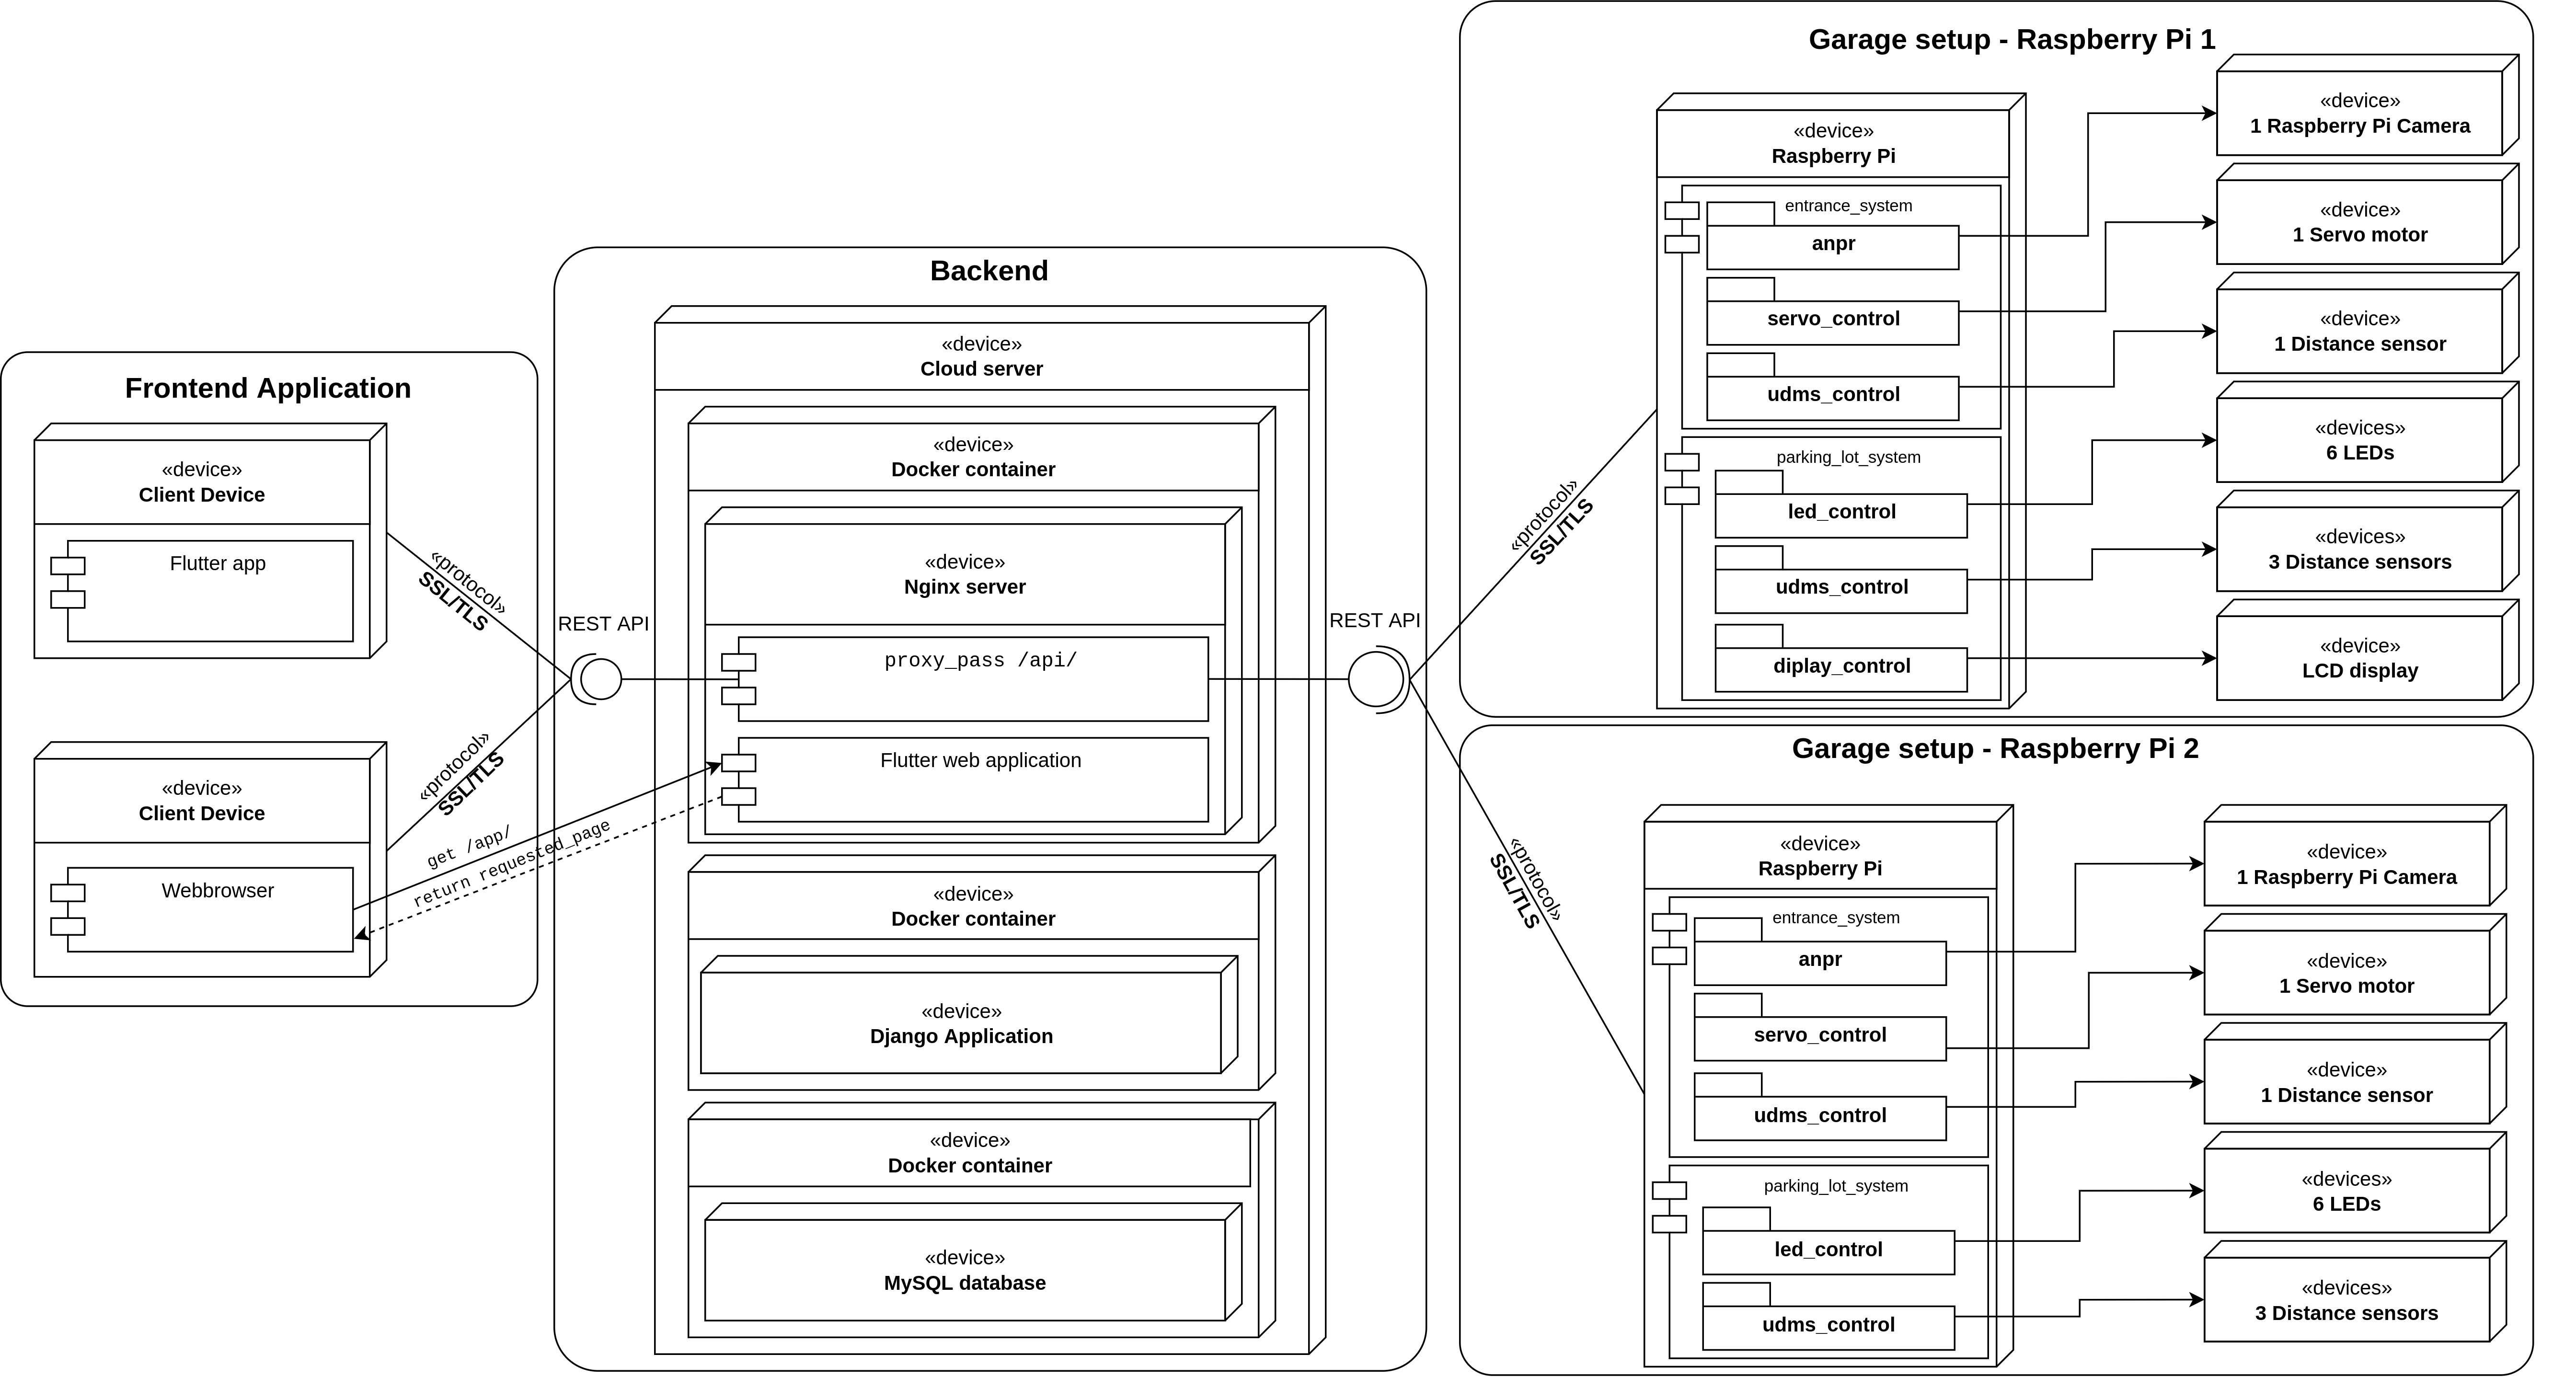
\includegraphics[width=25cm]{images/deployment_diagrams/deployment_diagram-general.drawio.png}
    \caption{General deployment diagram of the entire \ac{ips}.}
    \label{fig:general-deployment-diagram}
\end{figure}
\end{landscape}

\clearpage
\section{App diagrams}\label{app:app-diagram}
\begin{landscape}
   \begin{figure}
    \centering
    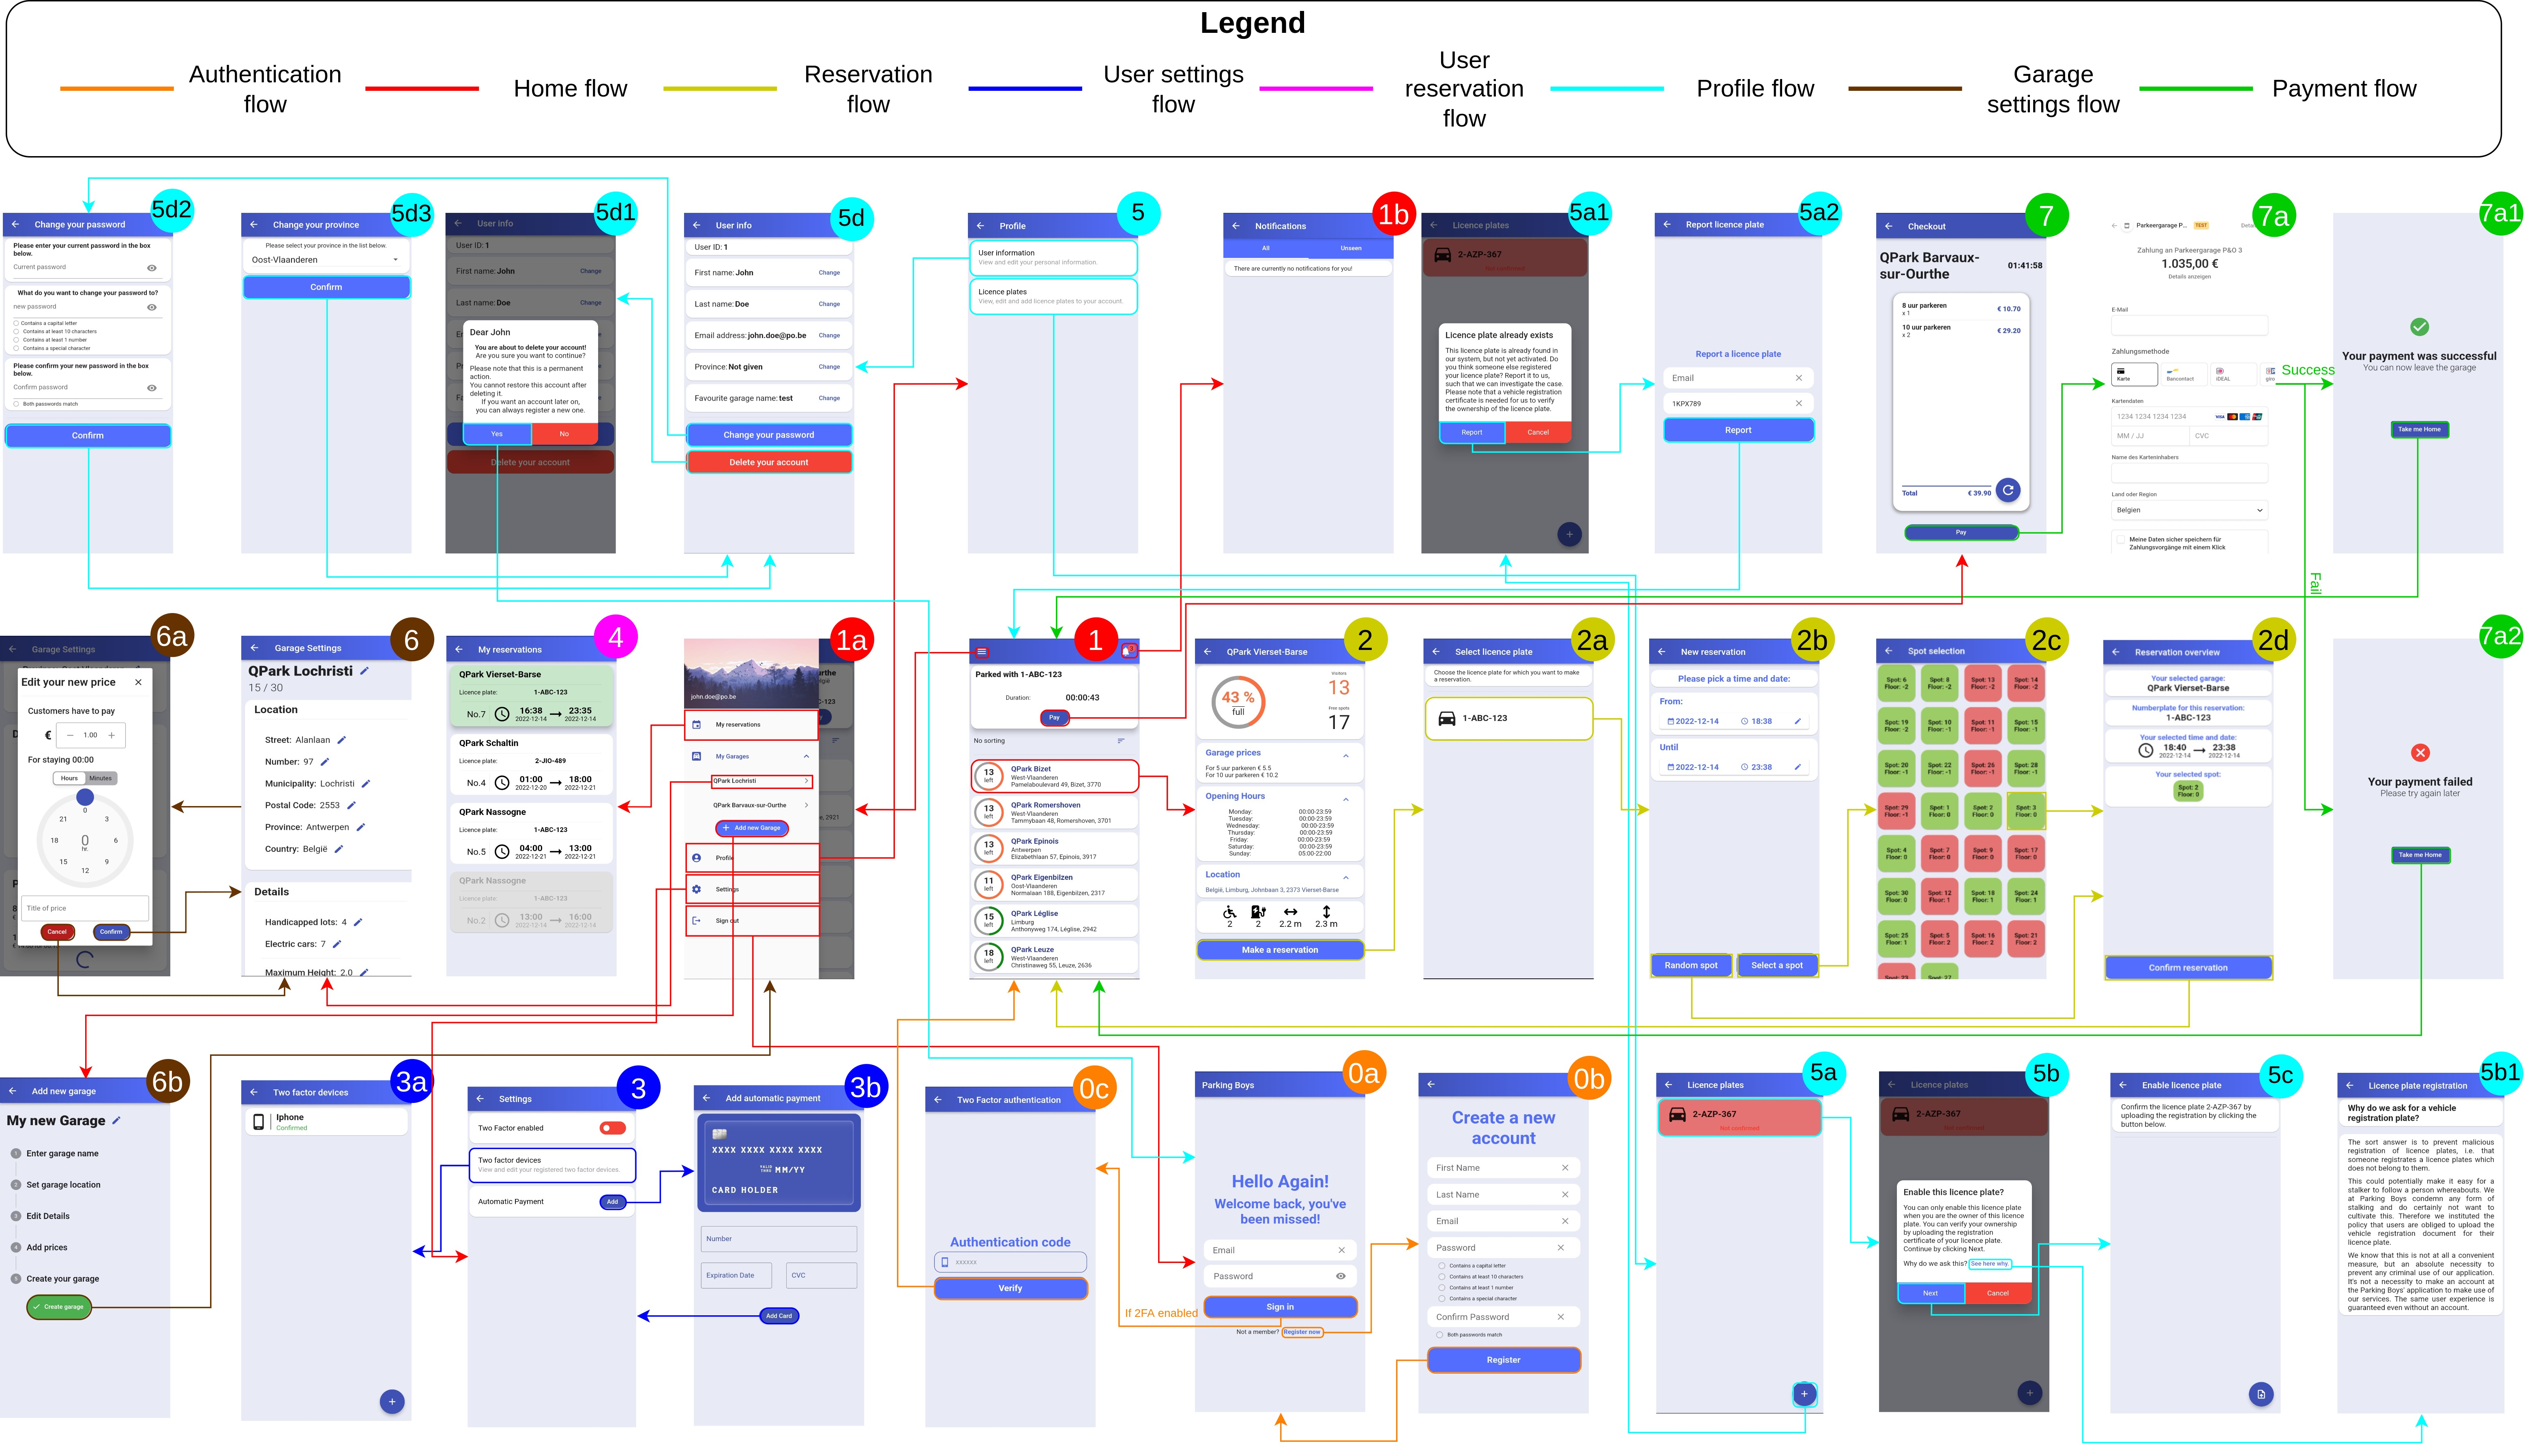
\includegraphics[width=25cm]{images/app/app_diagrams/app_diagram-general.jpg}
    \caption[General app diagram.]{General app diagram which displays the user flow within the frontend application. The pages are enumerated, where a new number indicates a change of flow. Pages with the same number belong to the same logic flow within the application. The routes of the back button are not indicated with an arrow as they represent the reverse direction of the arrow which points to this page.}
    \label{fig:general-app-diagram}
\end{figure}
\end{landscape}

\clearpage
\begin{figure}[hpt]
    \centering
    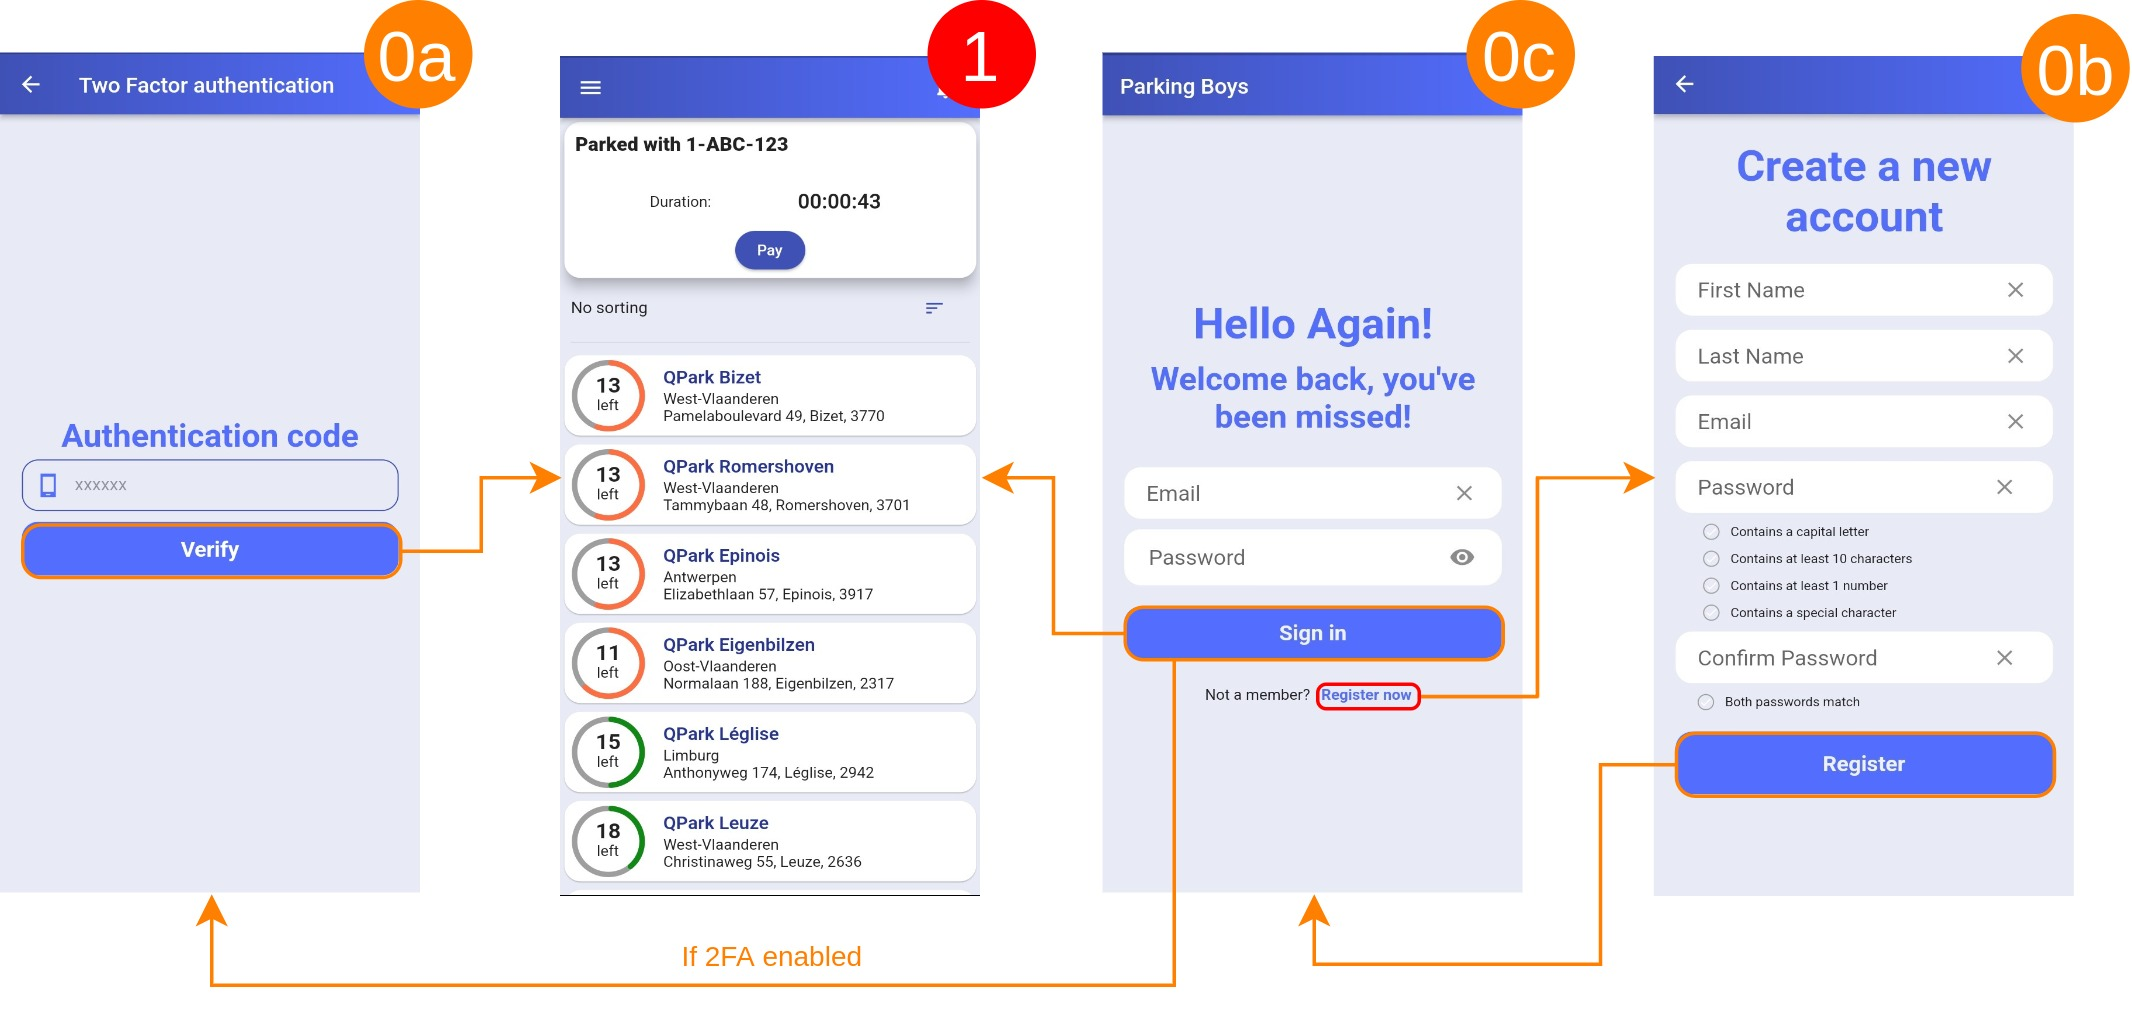
\includegraphics[width=16cm]{images/app/app_diagrams/app_diagram-auth-flow.jpg}
    \caption{App diagram of the authentication flow (Flow 0).}
    \label{fig:auth-flow}
\end{figure}
\begin{figure}[hpt]
    \centering
    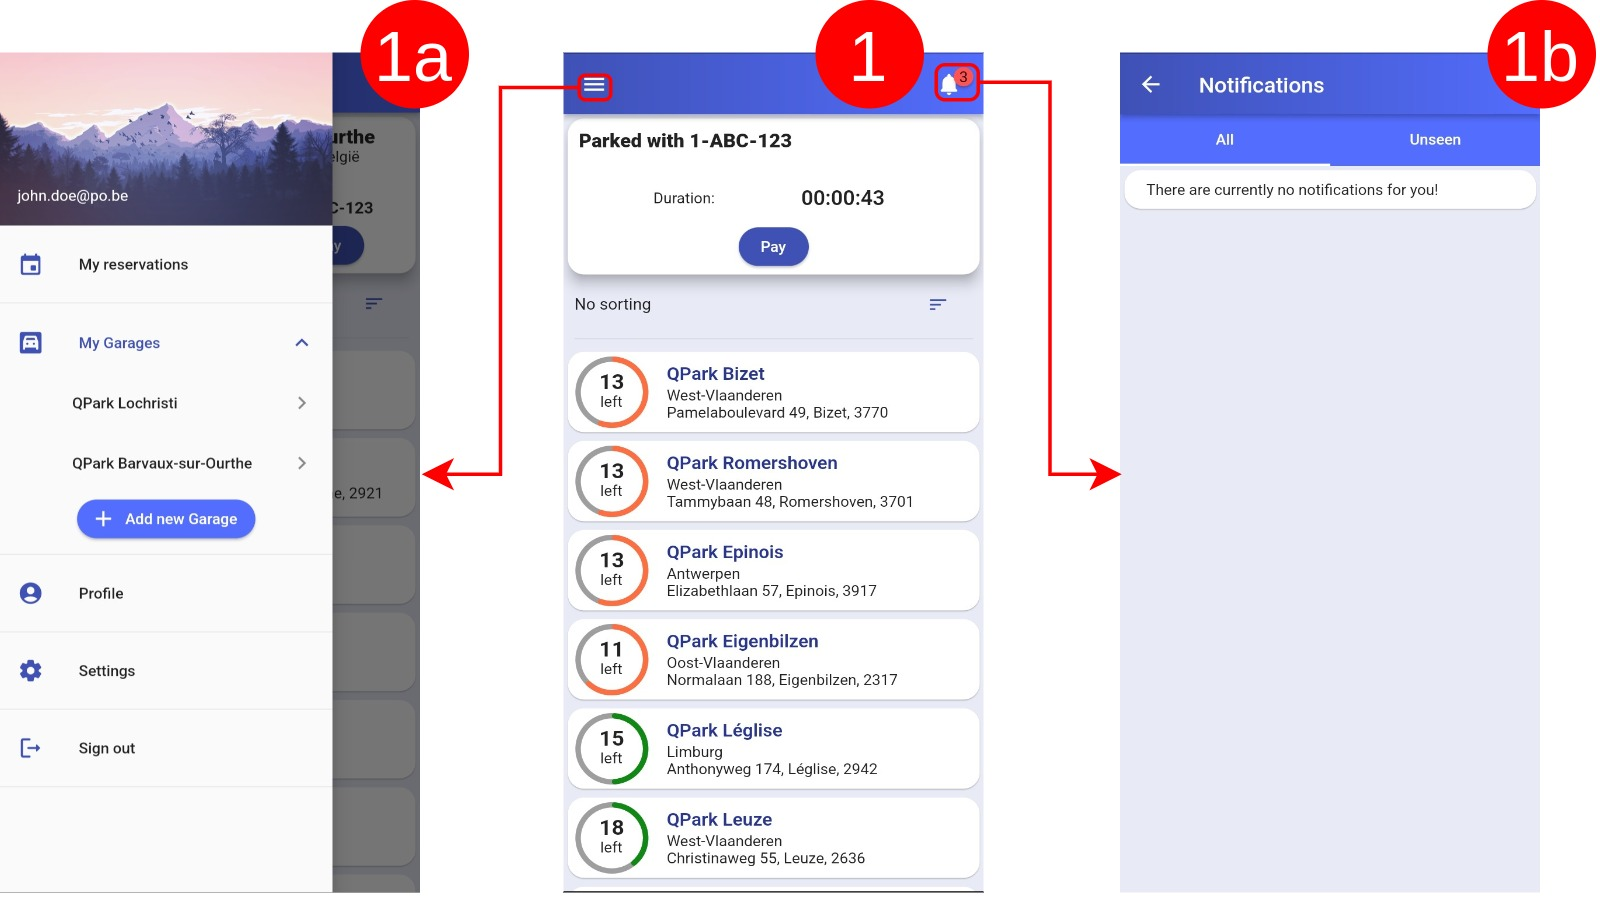
\includegraphics[width=16cm]{images/app/app_diagrams/app_diagram-home-flow.jpg}
    \caption{App diagram of the home flow (Flow 1).}
    \label{fig:home-flow}
\end{figure}

\clearpage

\begin{figure}[hpt]
    \centering
    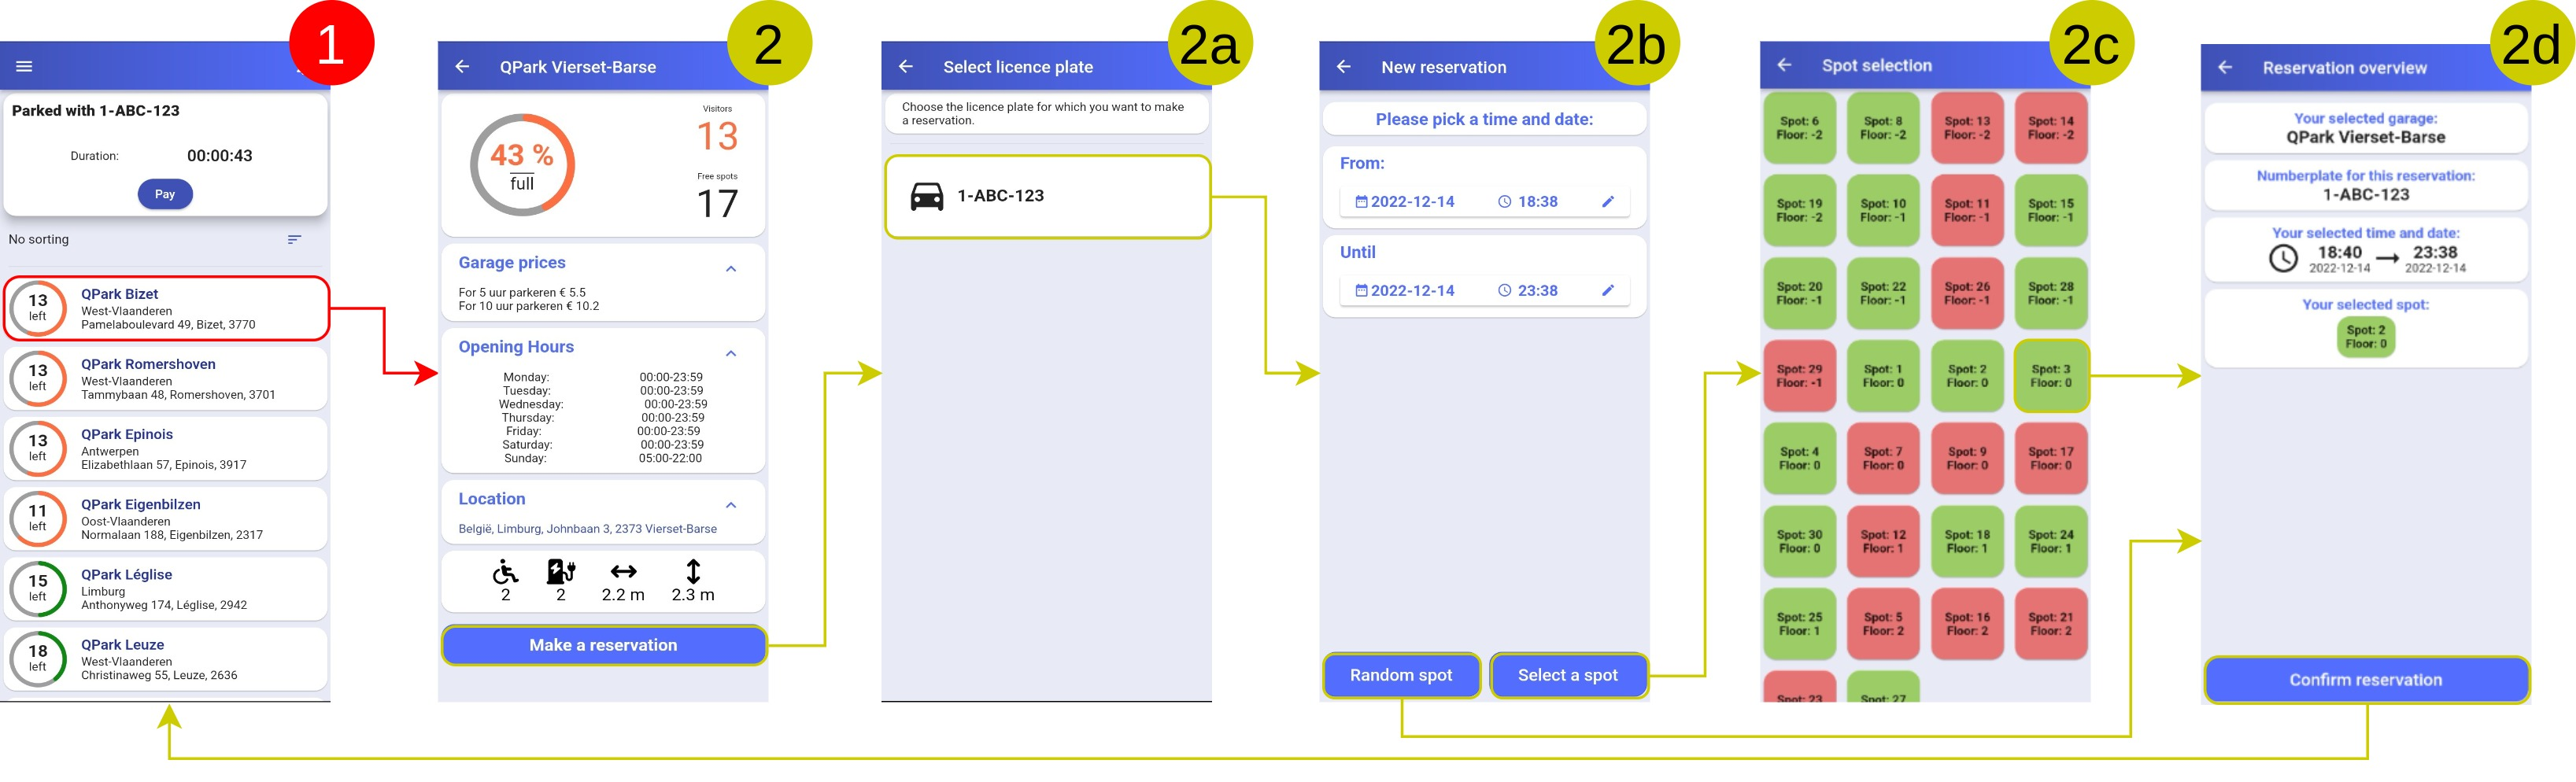
\includegraphics[width=14cm]{images/app/app_diagrams/app_diagram-reservation.jpg}
    \caption{App diagram of the reservation flow (Flow 2).}
    \label{fig:reservation-flow}
\end{figure}
\begin{figure}[hpt]
    \centering
    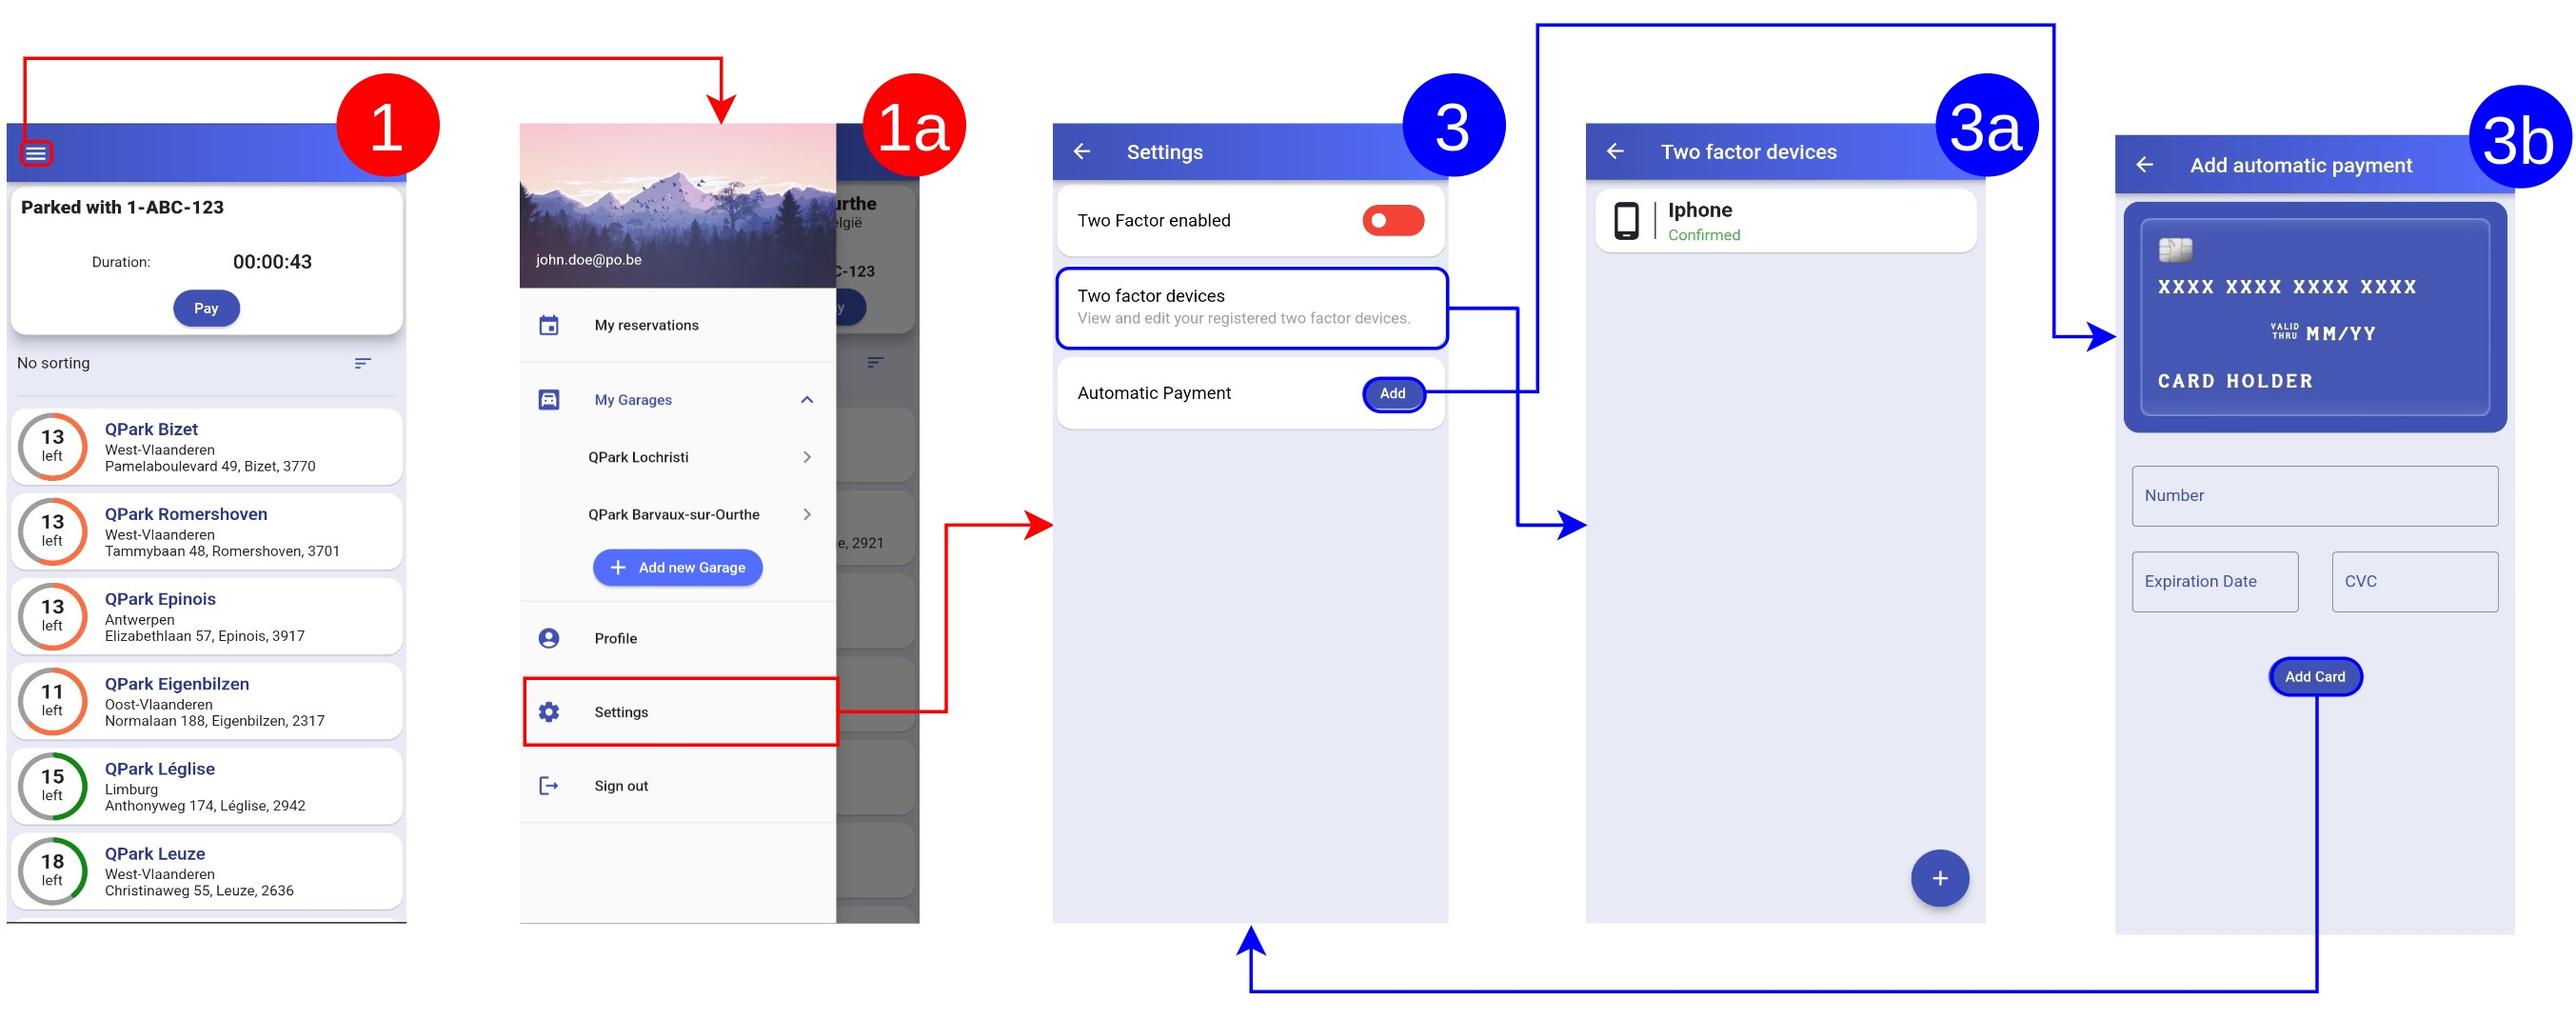
\includegraphics[width=14cm]{images/app/app_diagrams/app_diagram-user-settings-flow.jpg}
    \caption{App diagram of the user settings flow (Flow 3).}
    \label{fig:user-settings-flow}
\end{figure}
\begin{figure}[!hpt]
    \centering
    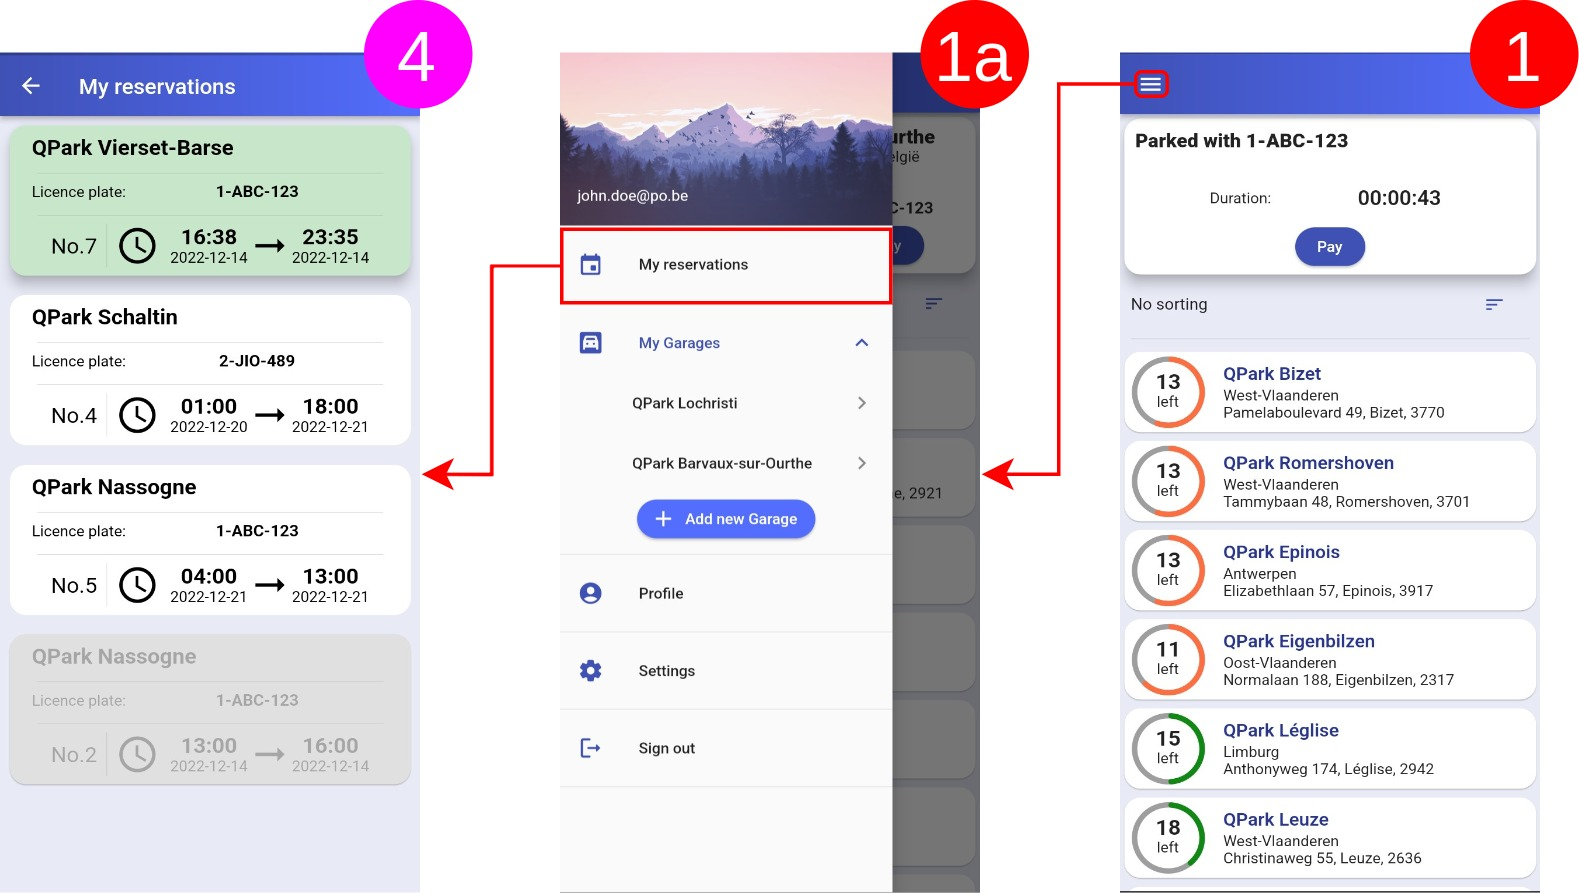
\includegraphics[width=14cm]{images/app/app_diagrams/app_diagram-user-reservation-flow.jpg}
    \caption{App diagram of the user reservation flow (Flow 4).}
    \label{fig:user-reservation-flow}
\end{figure}

\clearpage

\begin{figure}[hpt]
    \centering
    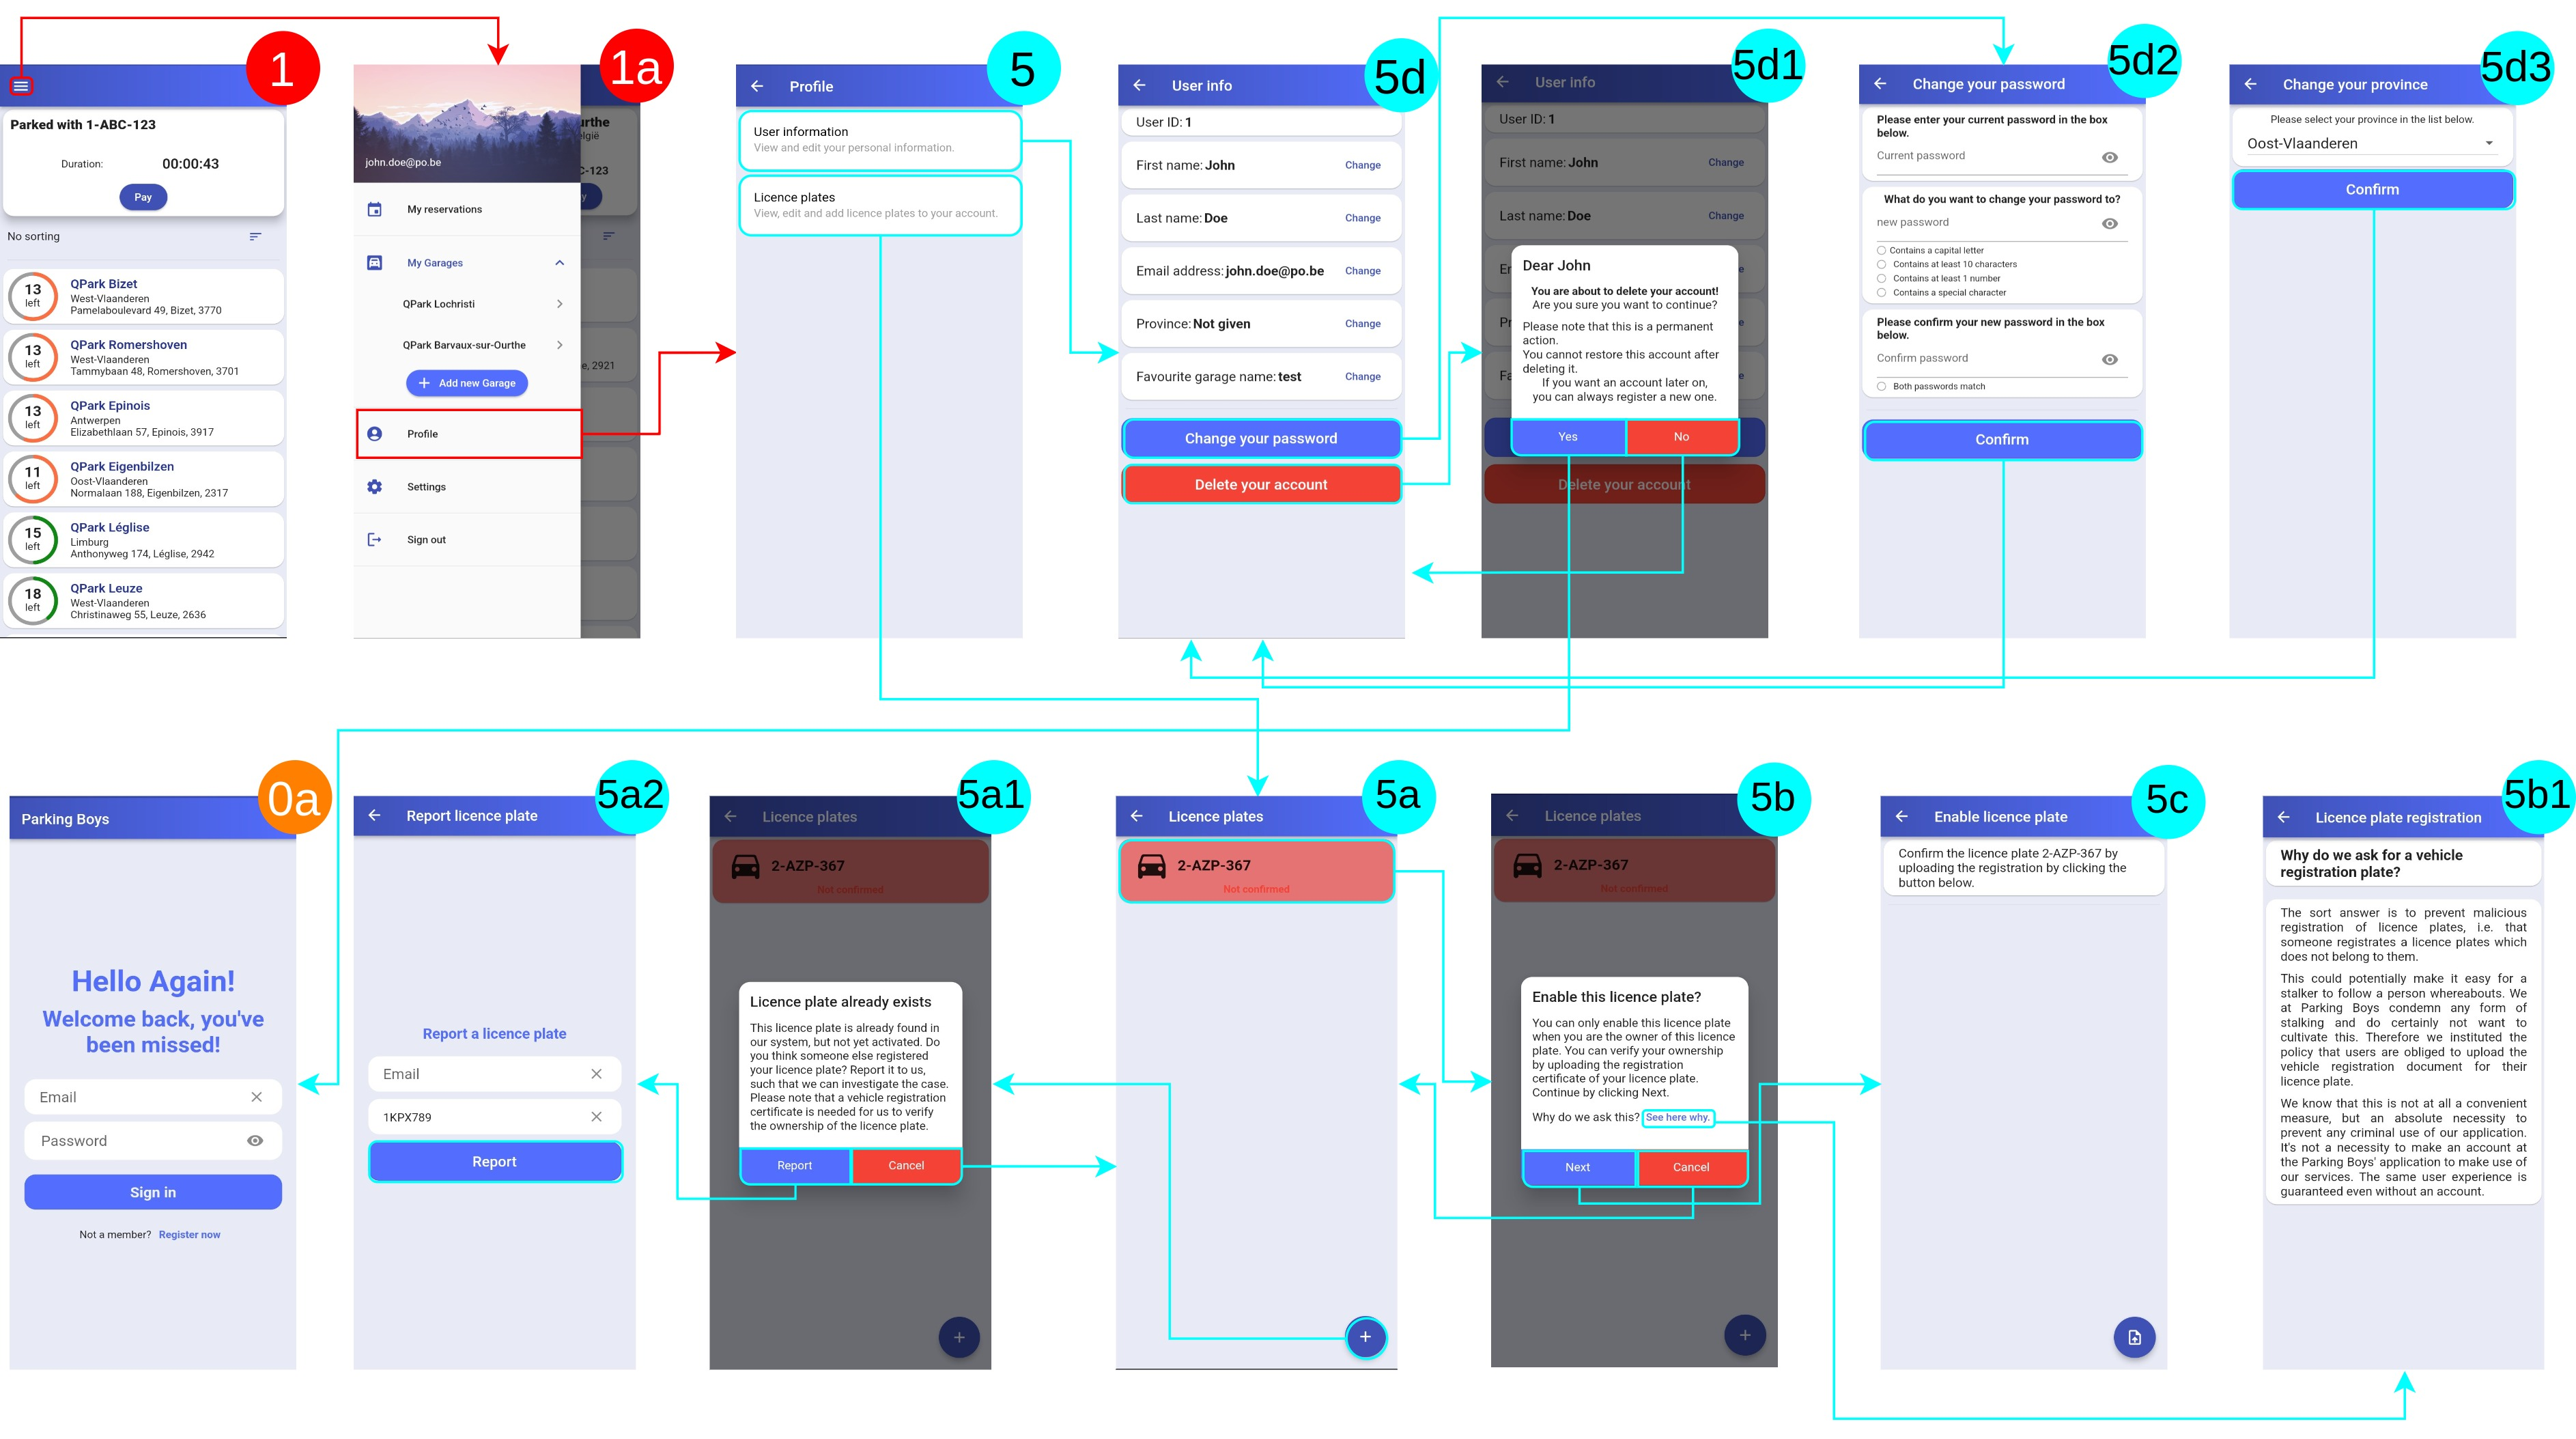
\includegraphics[width=16cm]{images/app/app_diagrams/app_diagram-profile-flow.jpg}
    \caption{App diagram of the profile flow (Flow 5).}
    \label{fig:profile-flow}
\end{figure}
\begin{figure}[hpt]
   \centering
   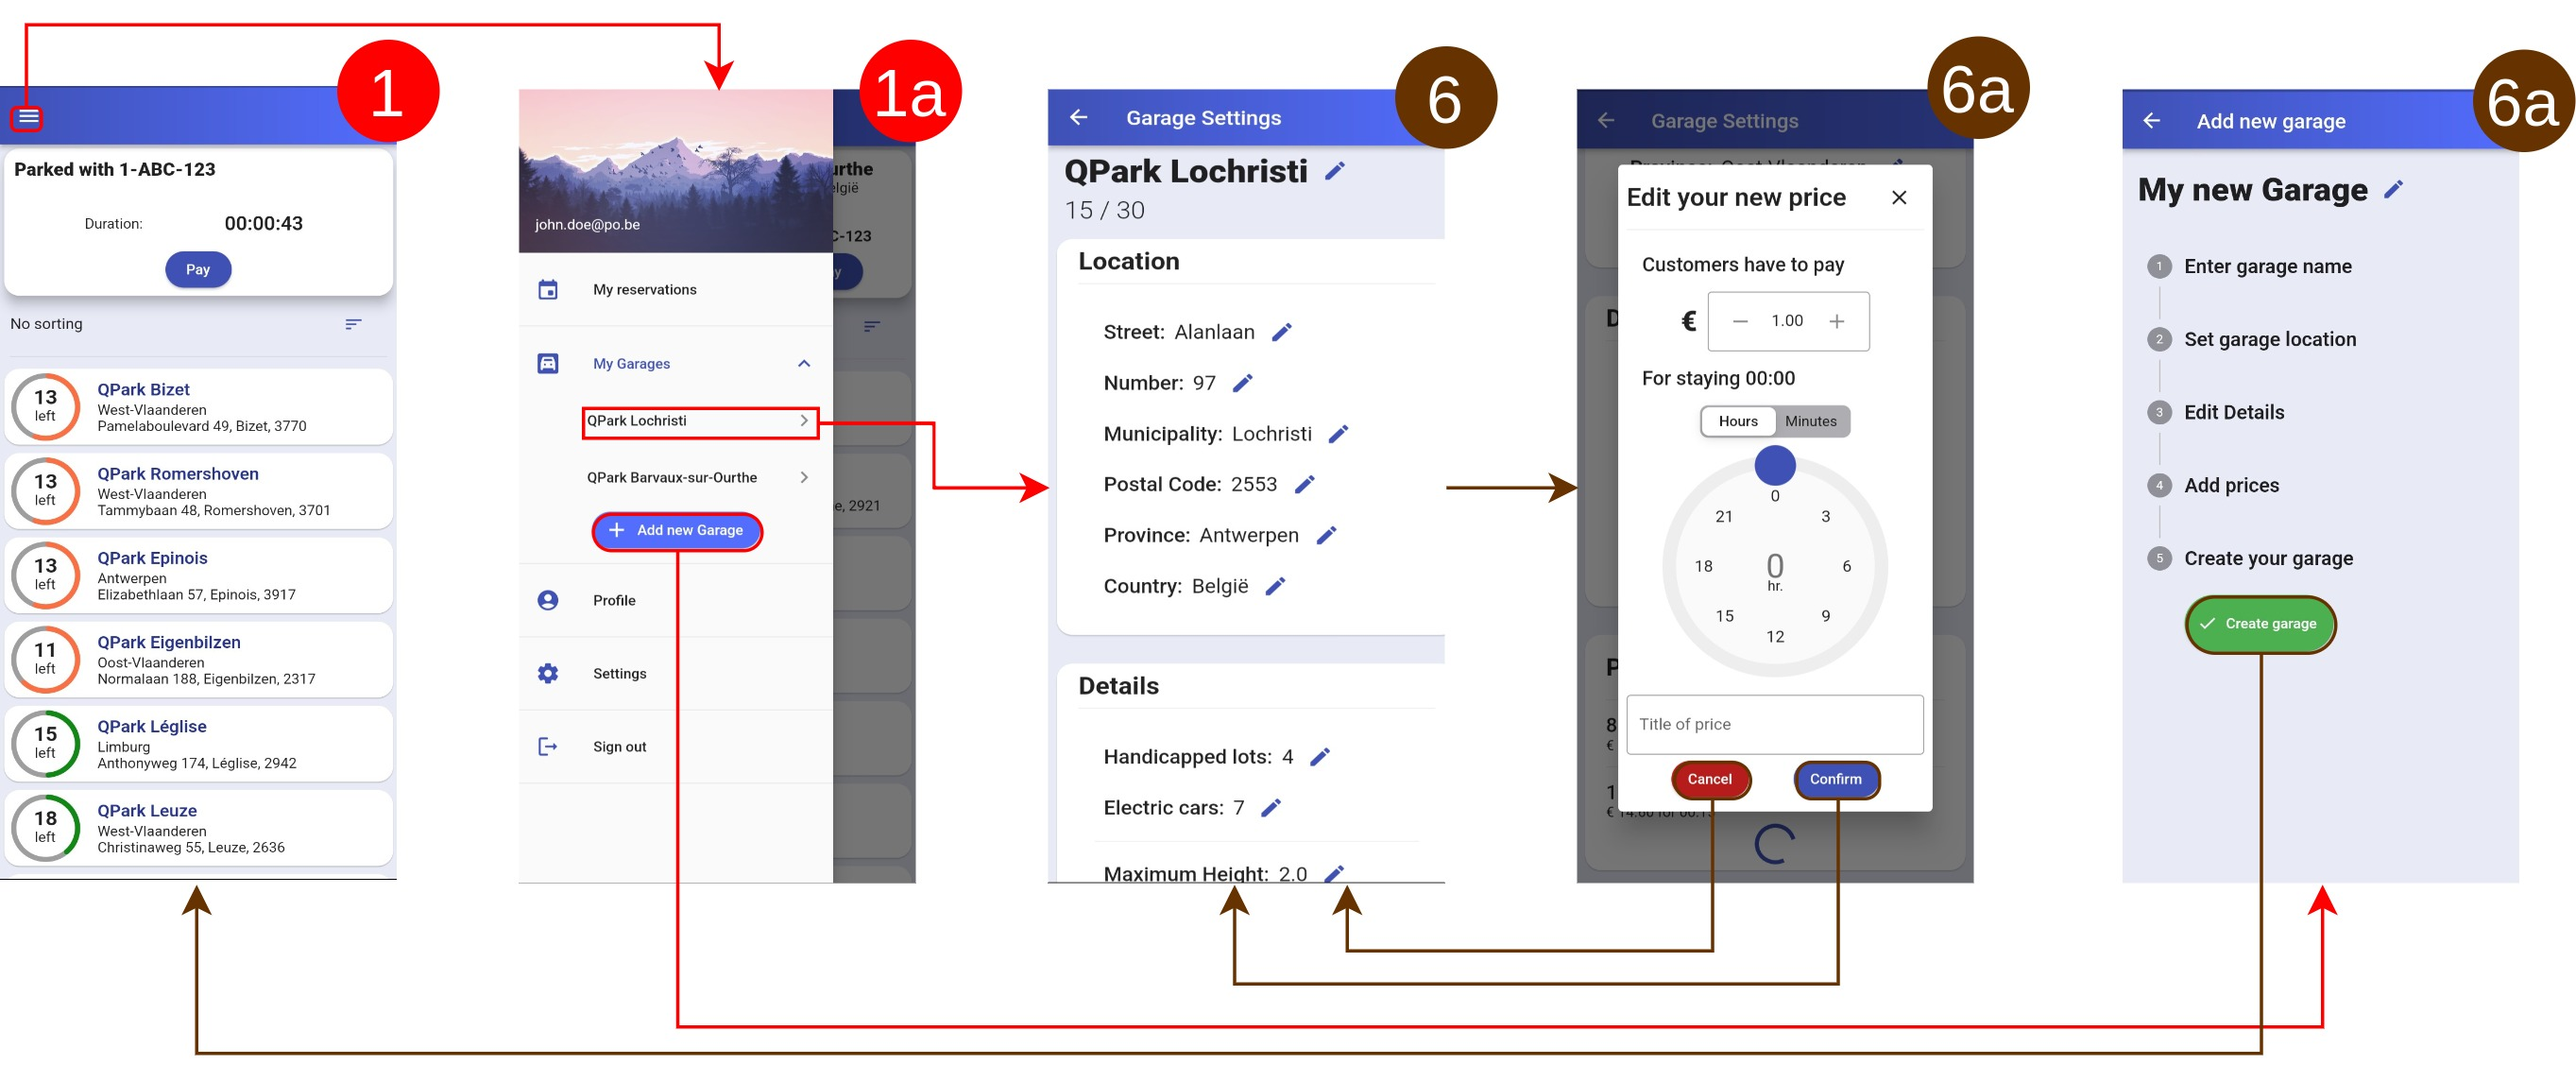
\includegraphics[width=16cm]{images/app/app_diagrams/app_diagram-garage-settings-flow.jpg}
    \caption{App diagram of the garage settings flow (Flow 6).}
   \label{fig:garage-settings-flow}
\end{figure}
\begin{figure}[!hpt]
    \centering
    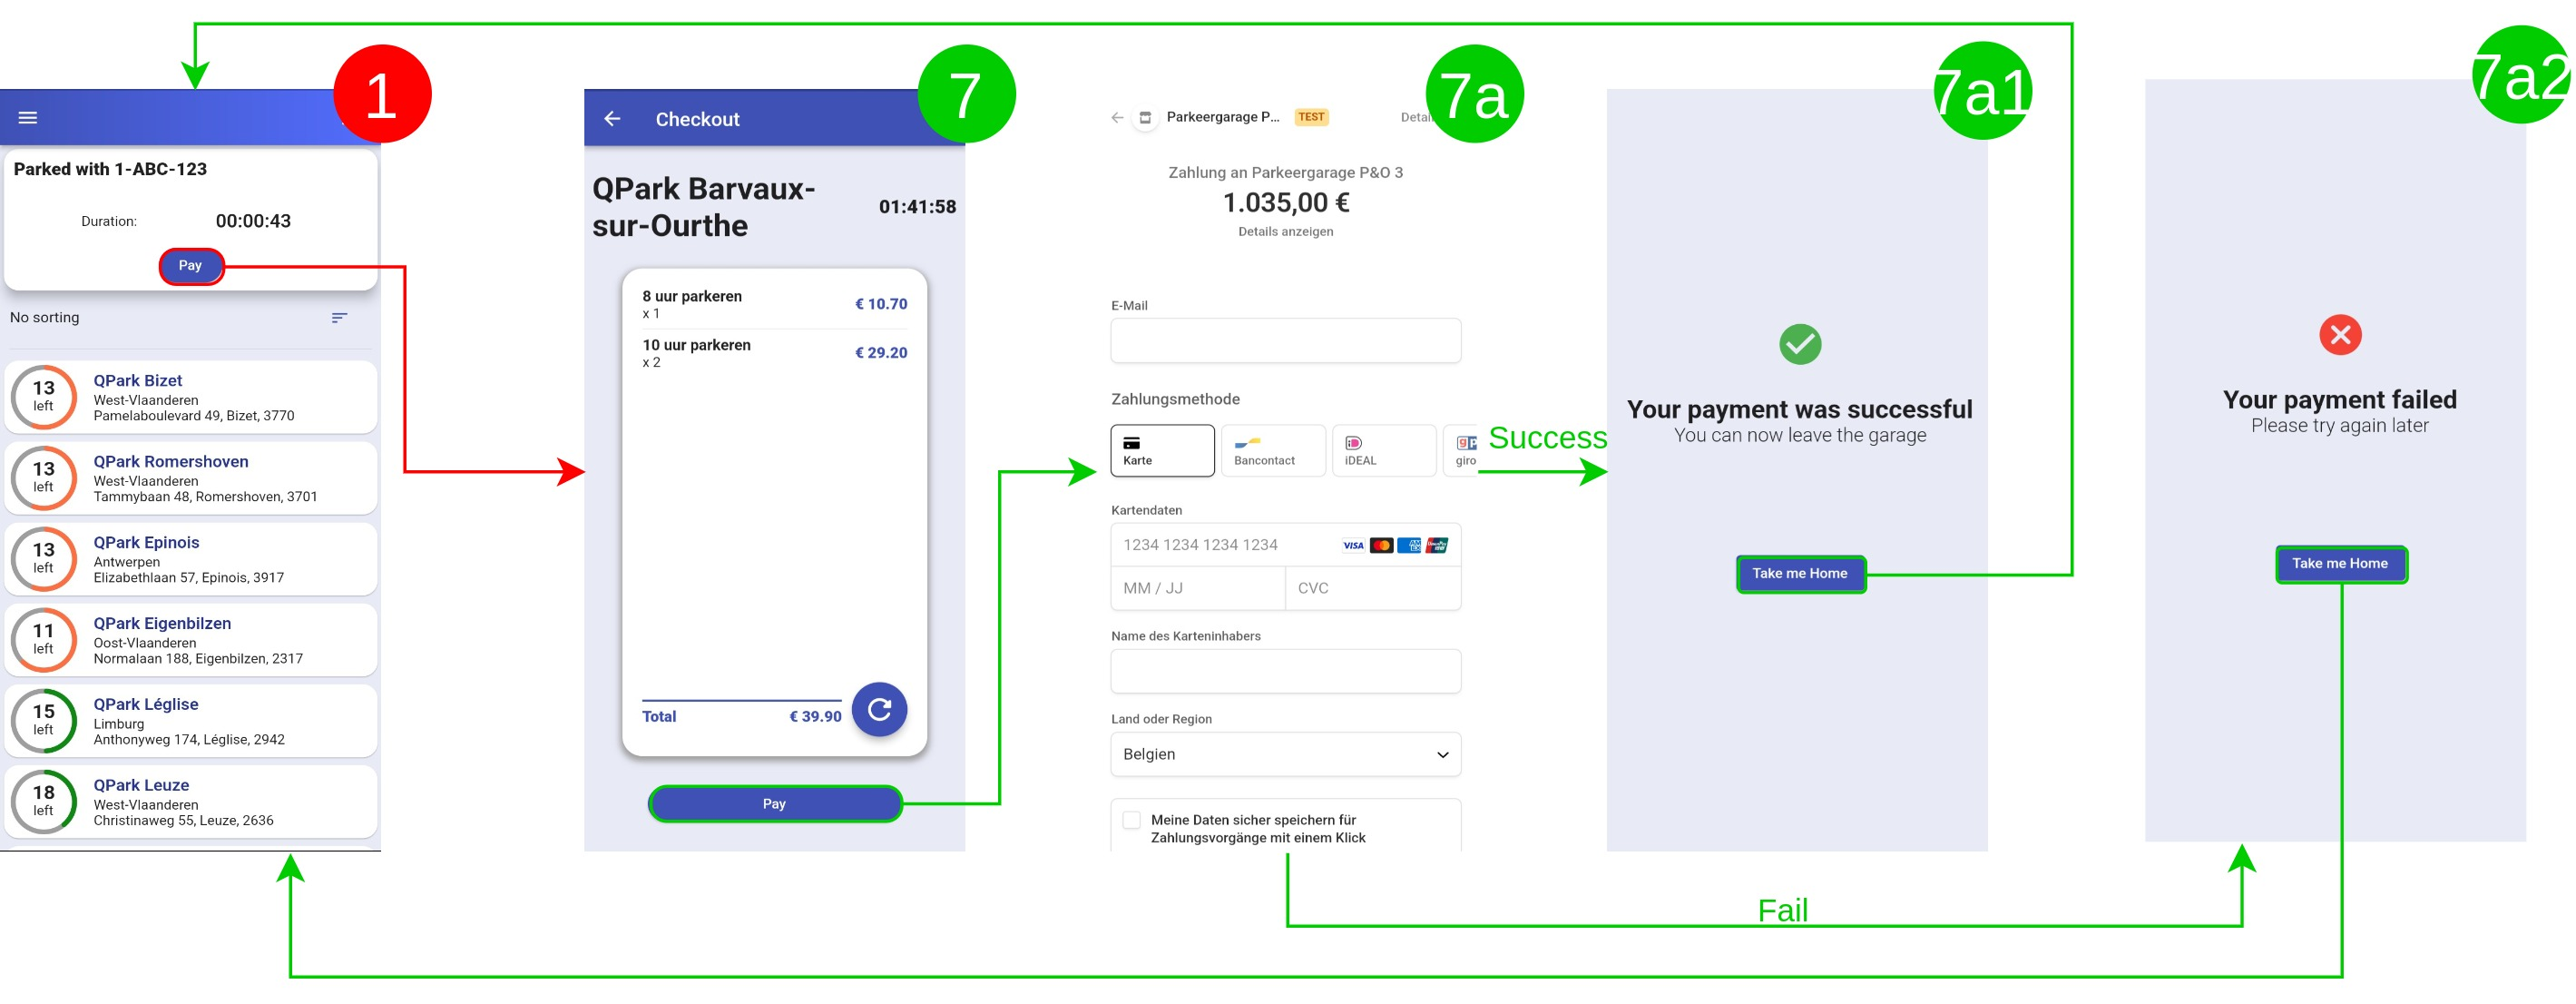
\includegraphics[width=16cm]{images/app/app_diagrams/app_diagram-payment.jpg}
    \caption{App diagram of the payment flow (Flow 7).}
    \label{fig:payment-flow}
\end{figure}

\clearpage

\begin{figure}[htp]
     \centering
     \begin{subfigure}[b]{0.30\textwidth}
         \centering
         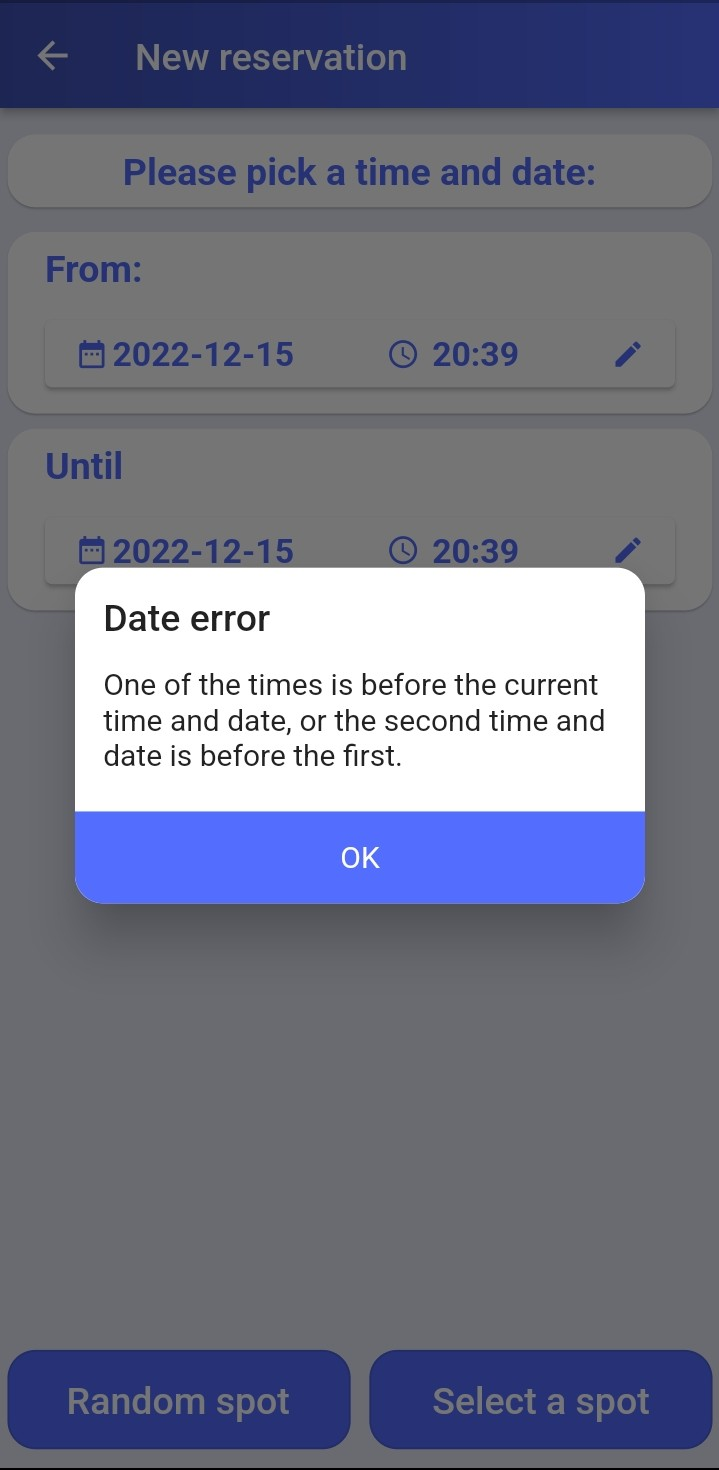
\includegraphics[width=\textwidth]{images/app/dialog1.jpg}
     \end{subfigure}
     \hfill
     \begin{subfigure}[b]{0.30\textwidth}
         \centering
         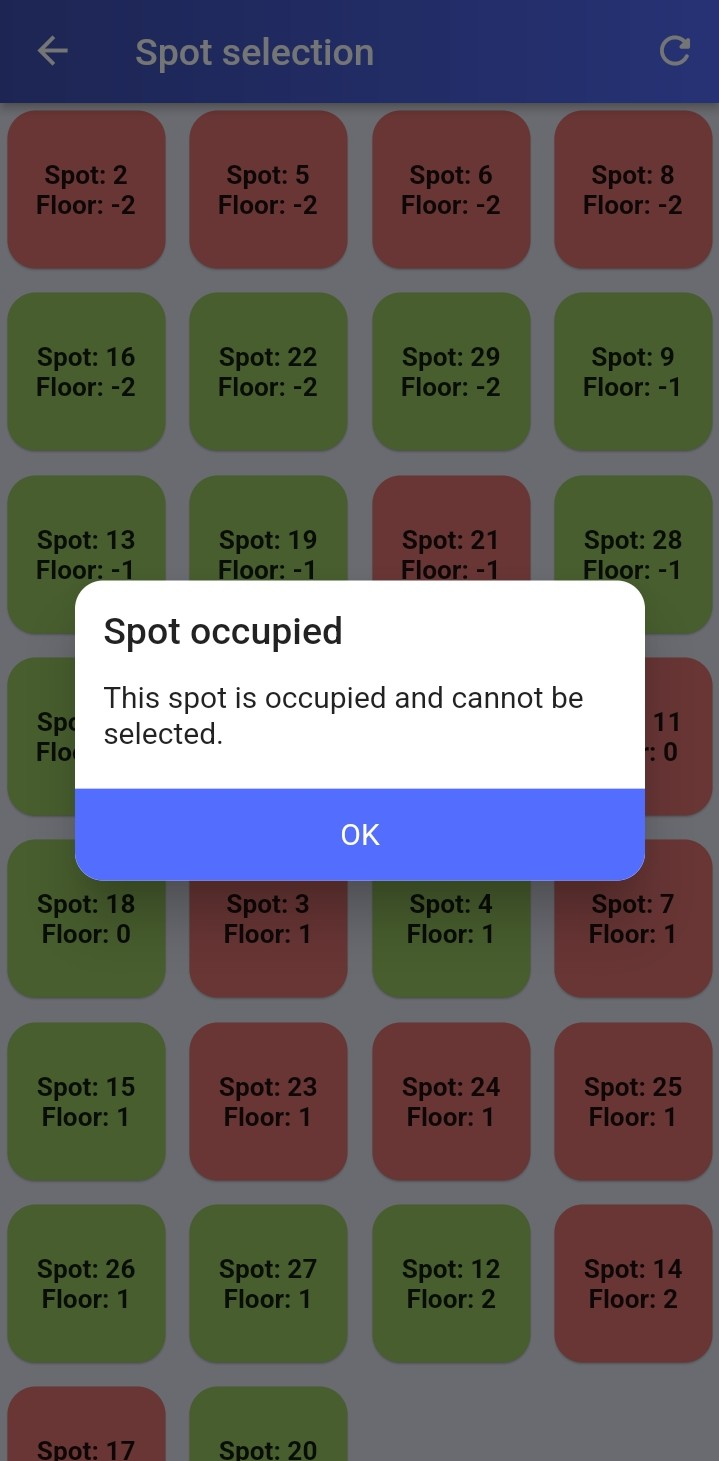
\includegraphics[width=\textwidth]{images/app/dialog2.jpg}
     \end{subfigure}
        \caption{Examples of error pop ups in the frontend application.}
        \label{fig:error-dialogs}
\end{figure}
\begin{figure}[!htp]
     \centering
     \begin{subfigure}[b]{0.30\textwidth}
         \centering
         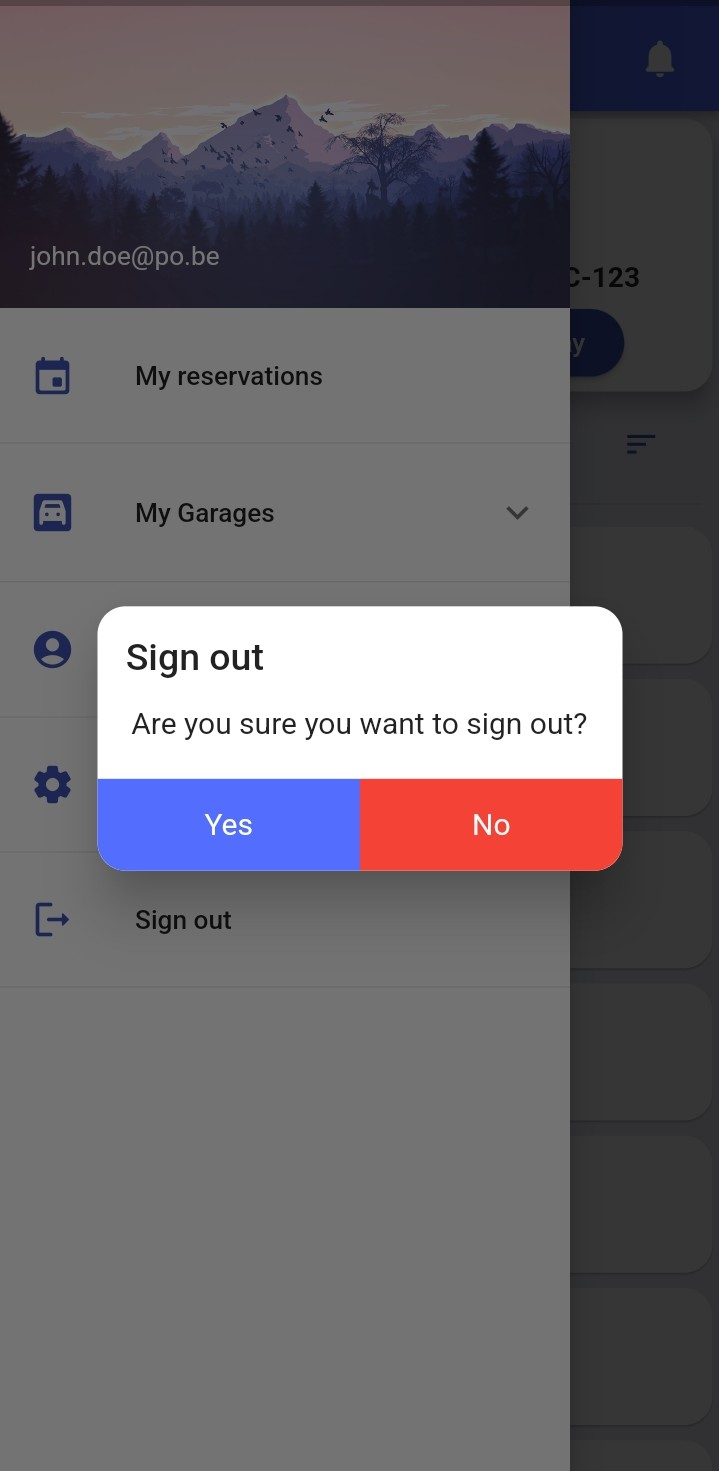
\includegraphics[width=\textwidth]{images/app/dialog3.jpg}
     \end{subfigure}
     \hfill
     \begin{subfigure}[b]{0.30\textwidth}
         \centering
         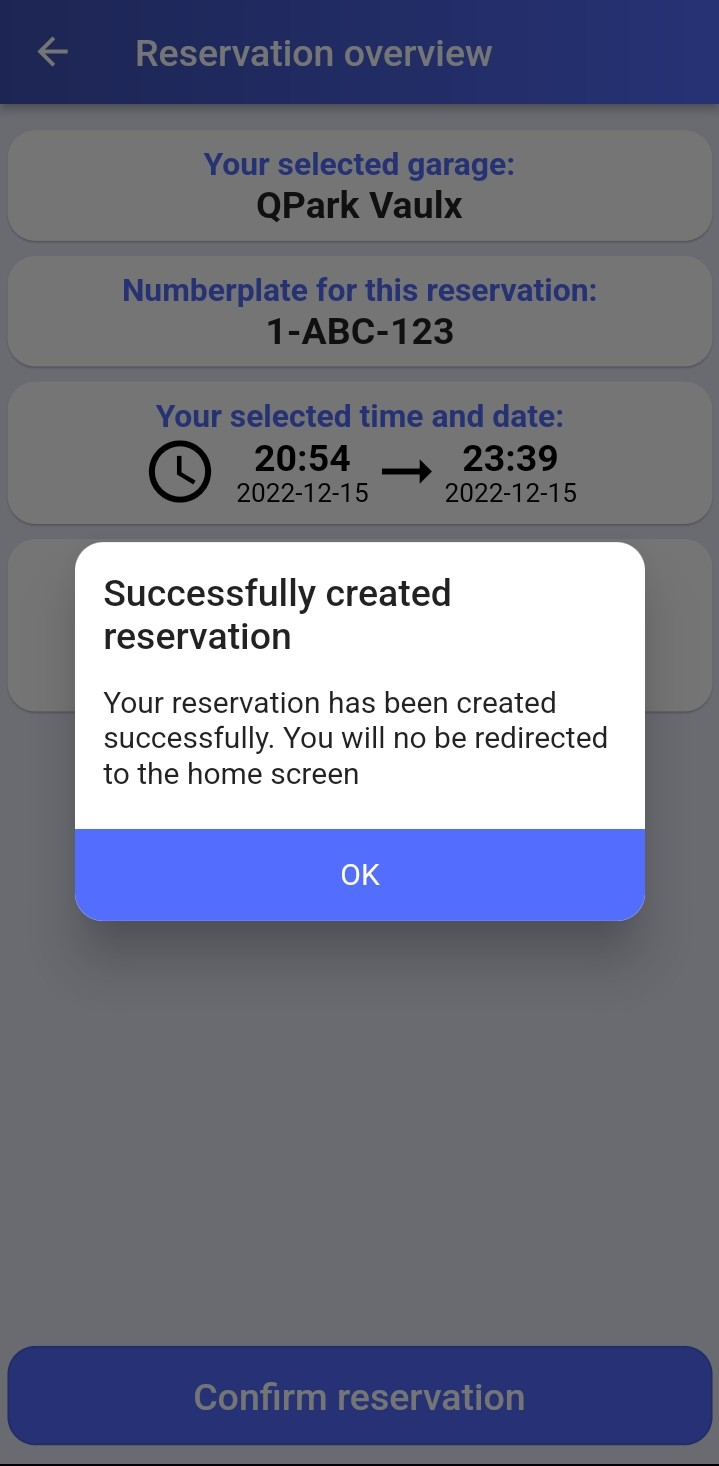
\includegraphics[width=\textwidth]{images/app/dialog4.jpg}
     \end{subfigure}
        \caption{Examples of information pop ups in the frontend application.}
        \label{fig:information-dialogs}
\end{figure}

\clearpage

\section{App pages}\label{app:app-pages}
\begin{table}
\centering
         \caption[An overview of all the different pages in the frontend application.]{An overview of all the different pages in the frontend application, together with their page code and a short description.}
        \label{tab:app-pages}

\begin{tabular}{|p{2cm}|p{4cm}|p{9cm}|}

         \hline
         \textbf{Page code}& \textbf{Page name} & \textbf{Short description} \\
         \hline
         \hline
         0a & Login page & Lets the user enter their email and password and authenticates it with the backend.\\
         \hline         
         0b & Register page & Allows the creation of new accounts by inputting all necessary information by the user.\\
         \hline 
         0c & \ac{2fa} Page & Allows the user to enter the \ac{2fa}-code from their \ac{totp}-device. \\
         \hline 
         \hline
         1 & Home page & Central page in the application which is the entry point for all major flows.\\
         \hline 
         1a & Home banner & Banner which allows the user to navigate to all important flows and to sign out. \\
         \hline 
         \hline
         2 & Garage info page & Provides an overview of all information about a garage, including its occupancy, prices and opening hours. Is the entry point for the reservation flow.\\
         \hline 
         2a & Licence plate selection page & Allows the user to select for which licence plate they want to make a reservation. \\
         \hline 
         2b & Make reservation page & Allows the user to enter their start and end time of the reservation they want to make. Validates them before continuing. \\
         \hline 
         2c & Spot selection page & Allows the user to choose a parking lot for which they want to make a reservation. \\
         \hline 
         2d & Reservation overview page &  Provides an overview of the reservation the user is about to make. On confirm, the user is redirected to the home page \\
         \hline 
         \hline
         3 & Settings page & Entry point for the users altering the user settings. \\
         \hline 
         3a & Two factor devices page & Allows the user to add, update or delete \ac{totp}-devices. \\
         \hline 
         3b & Add automatic payment page& Allows the user to enter their credit card details, which enables automatic payment.\\
         \hline 
         \hline
         4 & User reservation page & Overview of the user's reservations, highlighting the current reservation and disabling past reservations.\\
         \hline 
         \hline
         5 & Profile page & Entry point for altering and viewing user information. \\
         \hline 
         5a & Licence plates page & Allows the user to view, add and confirm licence plates. \\
         \hline 
         5b & Confirm licence plate dialog& Allows the user to choose to enable their licence plate. \\
         \hline 
         5b1 & Registration explication page & Explains the user why a vehicle registration document is necessary for the application to enable their licence plate.\\
         \hline 
         5c & Confirm licence plate page & Allows the user to upload a vehicle registration document to enable their licence plate. \\
         \hline 
         5d & User info page & Allows the user to view and edit their personal information. \\
         \hline 
         5d1 & User deletion pop up & Allows the user to choose if they want to delete their account. \\
         \hline 
         5d2 & Change password page & Allows the user to change their password by entering a new one. \\
         \hline
         5d3 & Change province page & Allows the user to change their location.\\
         \hline 
         \hline
         6 & Garage settings page & Allows a garage owner to alter the information about their garage, including the parking lots, prices, opening hours and location. \\
         \hline 
         6a & Add prices page & Allows a garage owner to add new prices to their garage. The prices will be synchronised with the Stripe servers.\\
         \hline
         6b & Add garage page & Allows a garage owner to add a new garage to the system. This page also allows to add opening hours, prices and a location to the garage.\\
         \hline 
    \end{tabular}
\end{table}
\clearpage

\begin{table}[ht!]
    \centering
    \begin{tabular}{|p{2cm}|p{4cm}|p{9cm}|}
         \hline
         7 & Checkout page & Provides an overview of the due amount and the parked time to the user.\\
         \hline 
         7a & Payment page & Allows the user to pay their parking bill. \\
         \hline 
         7a1 & Payment success page & Provides confirmation to the user that their payment was successful. \\
         \hline 
         7a2 & Payment failed page page & Provides confirmation to the user that their payment was unsuccessful. \\
         \hline
    \end{tabular}
\end{table}
\clearpage
\section{Mechanical part list}\label{app:part-list}

\begin{table}[htp]
    \centering
    \caption{Overview of all used mechanical components and their model number.}
    \begin{tabular}{|c|c|c|}
        \hline
         \textbf{Component name} & \textbf{Model number} & \textbf{Amount}  \\
         \hline
         \hline
         Raspberry Pi & Model 3B & 2 \\
         \hline
         \textsc{dorhea} Raspberry Pi Mini Kamera & \textsc{he0304-002} & 2 \\
         \hline
         Ultrasonic distance measuring sensor & \textsc{hc-sr04} & 8 \\
         \hline
         Micro servo motor & \textsc{oky8003} & 2 \\
         \hline
         Red \textsc{led} ($3 \ \text{mm}$) & \textsc{com-00533} & 6 \\
         \hline
         Green \textsc{led} ($3 \ \text{mm}$) & \textsc{com-09560} & 6 \\
         \hline
         Resistors ($20 \ \text{k}\Omega$) & \textsc{sfr2500002002fr500} & 12 \\
         \hline
         Jumper cables & / & $\approx 40$ \\
         \hline
         Raspberry Pi camera extension cable & \textsc{b087dfJ2rp} & 2 \\
         \hline
         LCD screen & ST7735 & 1 \\
         \hline
         \end{tabular}
    \label{tab:part_list}
\end{table}
\clearpage
\section{Backend API slugs}\label{app:backend-api-slugs}
\begin{table}[htp]
    \centering
    \begin{tabular}{|l|l|p{7cm}|}
        \hline
         \textbf{Slug} & \textbf{Methods} & \textbf{Short Description}  \\
         \hline
         \hline
         \texttt{api/user} &  \texttt{GET}, \texttt{PUT}, \texttt{DELETE} & Get, update or delete user information.\\
        \hline
        \texttt{api/user/change-password} &  \texttt{PUT} & Update a user's password, provided the old one.\\
        \hline
        \texttt{api/garages} &  \texttt{GET}, \texttt{POST}& Get all the available garages or post a new one.\\
        \hline
        \texttt{api/garage/<int:pk>} &  \texttt{GET}, \texttt{PUT}, \texttt{DELETE
        } & Get, update or delete information about a single garage.\\
        \hline
        \texttt{api/prices/<int:pk>} &  \texttt{GET}, \texttt{POST}, 
         & Get all the prices for a garage with id \texttt{pk} or post a new one.\\
        \hline
        \texttt{api/price/<int:pk>} &  \texttt{GET}, \texttt{PUT}, \texttt{DELETE}, 
         & Get, update or delete a price with id \texttt{pk}.\\
        \hline
        \texttt{api/opening-hours/<int:pk>} &  \texttt{GET}, \texttt{POST} & Get all the opening hours for a garage with id \texttt{pk} or add a new one.\\
        \hline
        \texttt{api/opening-hour/<int:pk>} & \texttt{GET}, \texttt{PUT}, \texttt{DELETE} & Get, update or delete opening hours with id \texttt{pk}.\\
        \hline
        \texttt{api/parking-lots/<int:pk>} &  \texttt{GET}, \texttt{POST} & Get all the parking lots for a garage with id \texttt{pk} or post a new one.\\
        \hline
        \texttt{api/parking-lot/<int:pk>} &  \texttt{GET}, \texttt{PUT}, \texttt{DELETE
        } & Get update or delete a parking lot with id \texttt{pk}. \\
        \hline
        \texttt{api/assign-parking-lot/<int:pk>} &  \texttt{GET} & Get a random free parking lot in the garage with id \texttt{pk}, given a start and end date. \\
        \hline
        \texttt{api/garage-settings/<int:pk>} &  \texttt{GET}, \texttt{PUT}, \texttt{DELETE
        } & Get, update or delete the garage settings of a garage with id \texttt{pk}.\\
        \hline
        \texttt{api/licence-plates} &  \texttt{GET}, \texttt{POST} & Get all licence plates for a user or add a new one.\\
        \hline
        \texttt{api/licence-plate/<int:pk>} &  \texttt{GET}, \texttt{PUT}, \texttt{DELETE} & Get, update or delete a licence plate with id \texttt{pk}. \\
        \hline
        \texttt{api/reservations} &  \texttt{GET}, \texttt{POST} & Get all user's reservations or add a new one.\\
        \hline
        \texttt{api/reservation/<int:pk>} &  \texttt{GET}, \texttt{PUT}, \texttt{DELETE
        } & Get, update or delete a reservation with id \texttt{pk}.\\
        \hline
        \texttt{api/notifications/<int:pk>} &  \texttt{GET} & Get all user's notifications.\\
        \hline
        \texttt{api/notification/<int:pk>} &  \texttt{PUT}, \texttt{DELETE
        } & Update or delete a notification with id \texttt{pk}.\\
        \hline
        \end{tabular}
    \caption{Overview of all general \ac{url} slugs which are supported by the backend application.}
    \label{tab:general-url}
\end{table}


\begin{table}[htp]
    \centering
    \begin{tabular}{|l|l|p{7cm}|}
    \hline
    \textbf{Slug} & \textbf{Methods} & \textbf{Short Description}  \\
    \hline
    \hline
        \texttt{api/auth/login} &  \texttt{POST} & Login a user given a email and password.\\
        \hline
        \texttt{api/auth/logout} &  \texttt{POST} & Logout a user, deleting its auth token.\\
        \hline
        \texttt{api/auth/activate-account} &  \texttt{GET} & Activate a user's account.\\
        \hline
        \texttt{api/auth/totp/disable} &  \texttt{POST} & Disable \ac{2fa} for a user.\\
        \hline
        \texttt{api/auth/totp} &  \texttt{GET}, \texttt{POST} & Get all the user's \ac{totp}-devices or add a new one.\\
        \hline
        \texttt{api/auth/totp/<int:pk>} &  \texttt{PUT}, \texttt{DELETE} & Update or delete a \ac{totp}-device with id \texttt{pk}.\\
        \hline
        \texttt{api/auth/totp/login/<int:code>} & \texttt{POST} & Post the \ac{2fa}-code to verify the user (\texttt{code} is a six-digit number).\\
        \hline
    \end{tabular}
    \caption{Overview of all \ac{url} slugs for authentication which are supported by the backend application.}
    \label{tab:auth-url}
\end{table}


\begin{table}[ht!]
    \centering
    \begin{tabular}{|l|l|p{7cm}|}
        \hline
    \textbf{Slug} & \textbf{Methods} & \textbf{Short Description}  \\
    \hline
        \hline
        \texttt{api/rpi/images} &  \texttt{POST} & Post the image taken by the Raspberry Pi to the backend for image analysis.\\
        \hline
        \texttt{api/rpi/parking-lot} &  \texttt{GET} & Get the parking lots from the garage where the Raspberry Pi is installed.\\
        \hline
            \end{tabular}
    \caption{Overview of all \ac{url} slugs for the local garage system, which are supported by the backend application.}
    \label{tab:url-rpi}
\end{table}


\begin{table}[ht!]
    \centering
    \begin{tabular}{|l|l|p{7cm}|}
        \hline
    \textbf{Slug} & \textbf{Methods} & \textbf{Short Description}  \\
    \hline
        \hline
        \texttt{api/checkout/create-session} &  \texttt{POST} & Create a checkout session for the user to pay.\\
        \hline
        \texttt{api/checkout/preview} &  \texttt{GET} & Get the items which the user has to pay (i.e. time quantities parked).\\
        \hline
        \texttt{api/checkout/webhook} &  \texttt{POST} & Listen to incoming requests from the Stripe servers for checkout updates.\\
        \hline
        \texttt{api/stripe-connection} &  \texttt{POST}, \texttt{DELETE} & Add or remove customers from Stripe.\\
        \hline
        \texttt{api/invoice/webhook} &  \texttt{GET} & Listen to invoice updates from the Stripe servers.\\
        \hline
    \end{tabular}
    \caption{Overview of all \ac{url} slugs for payment which are supported by the backend application.}
    \label{tab:url-payment}
\end{table}

\clearpage
\section{Sequence diagrams}\label{app:sequence-diagrams}

\begin{figure}[!hpt]
    \centering
    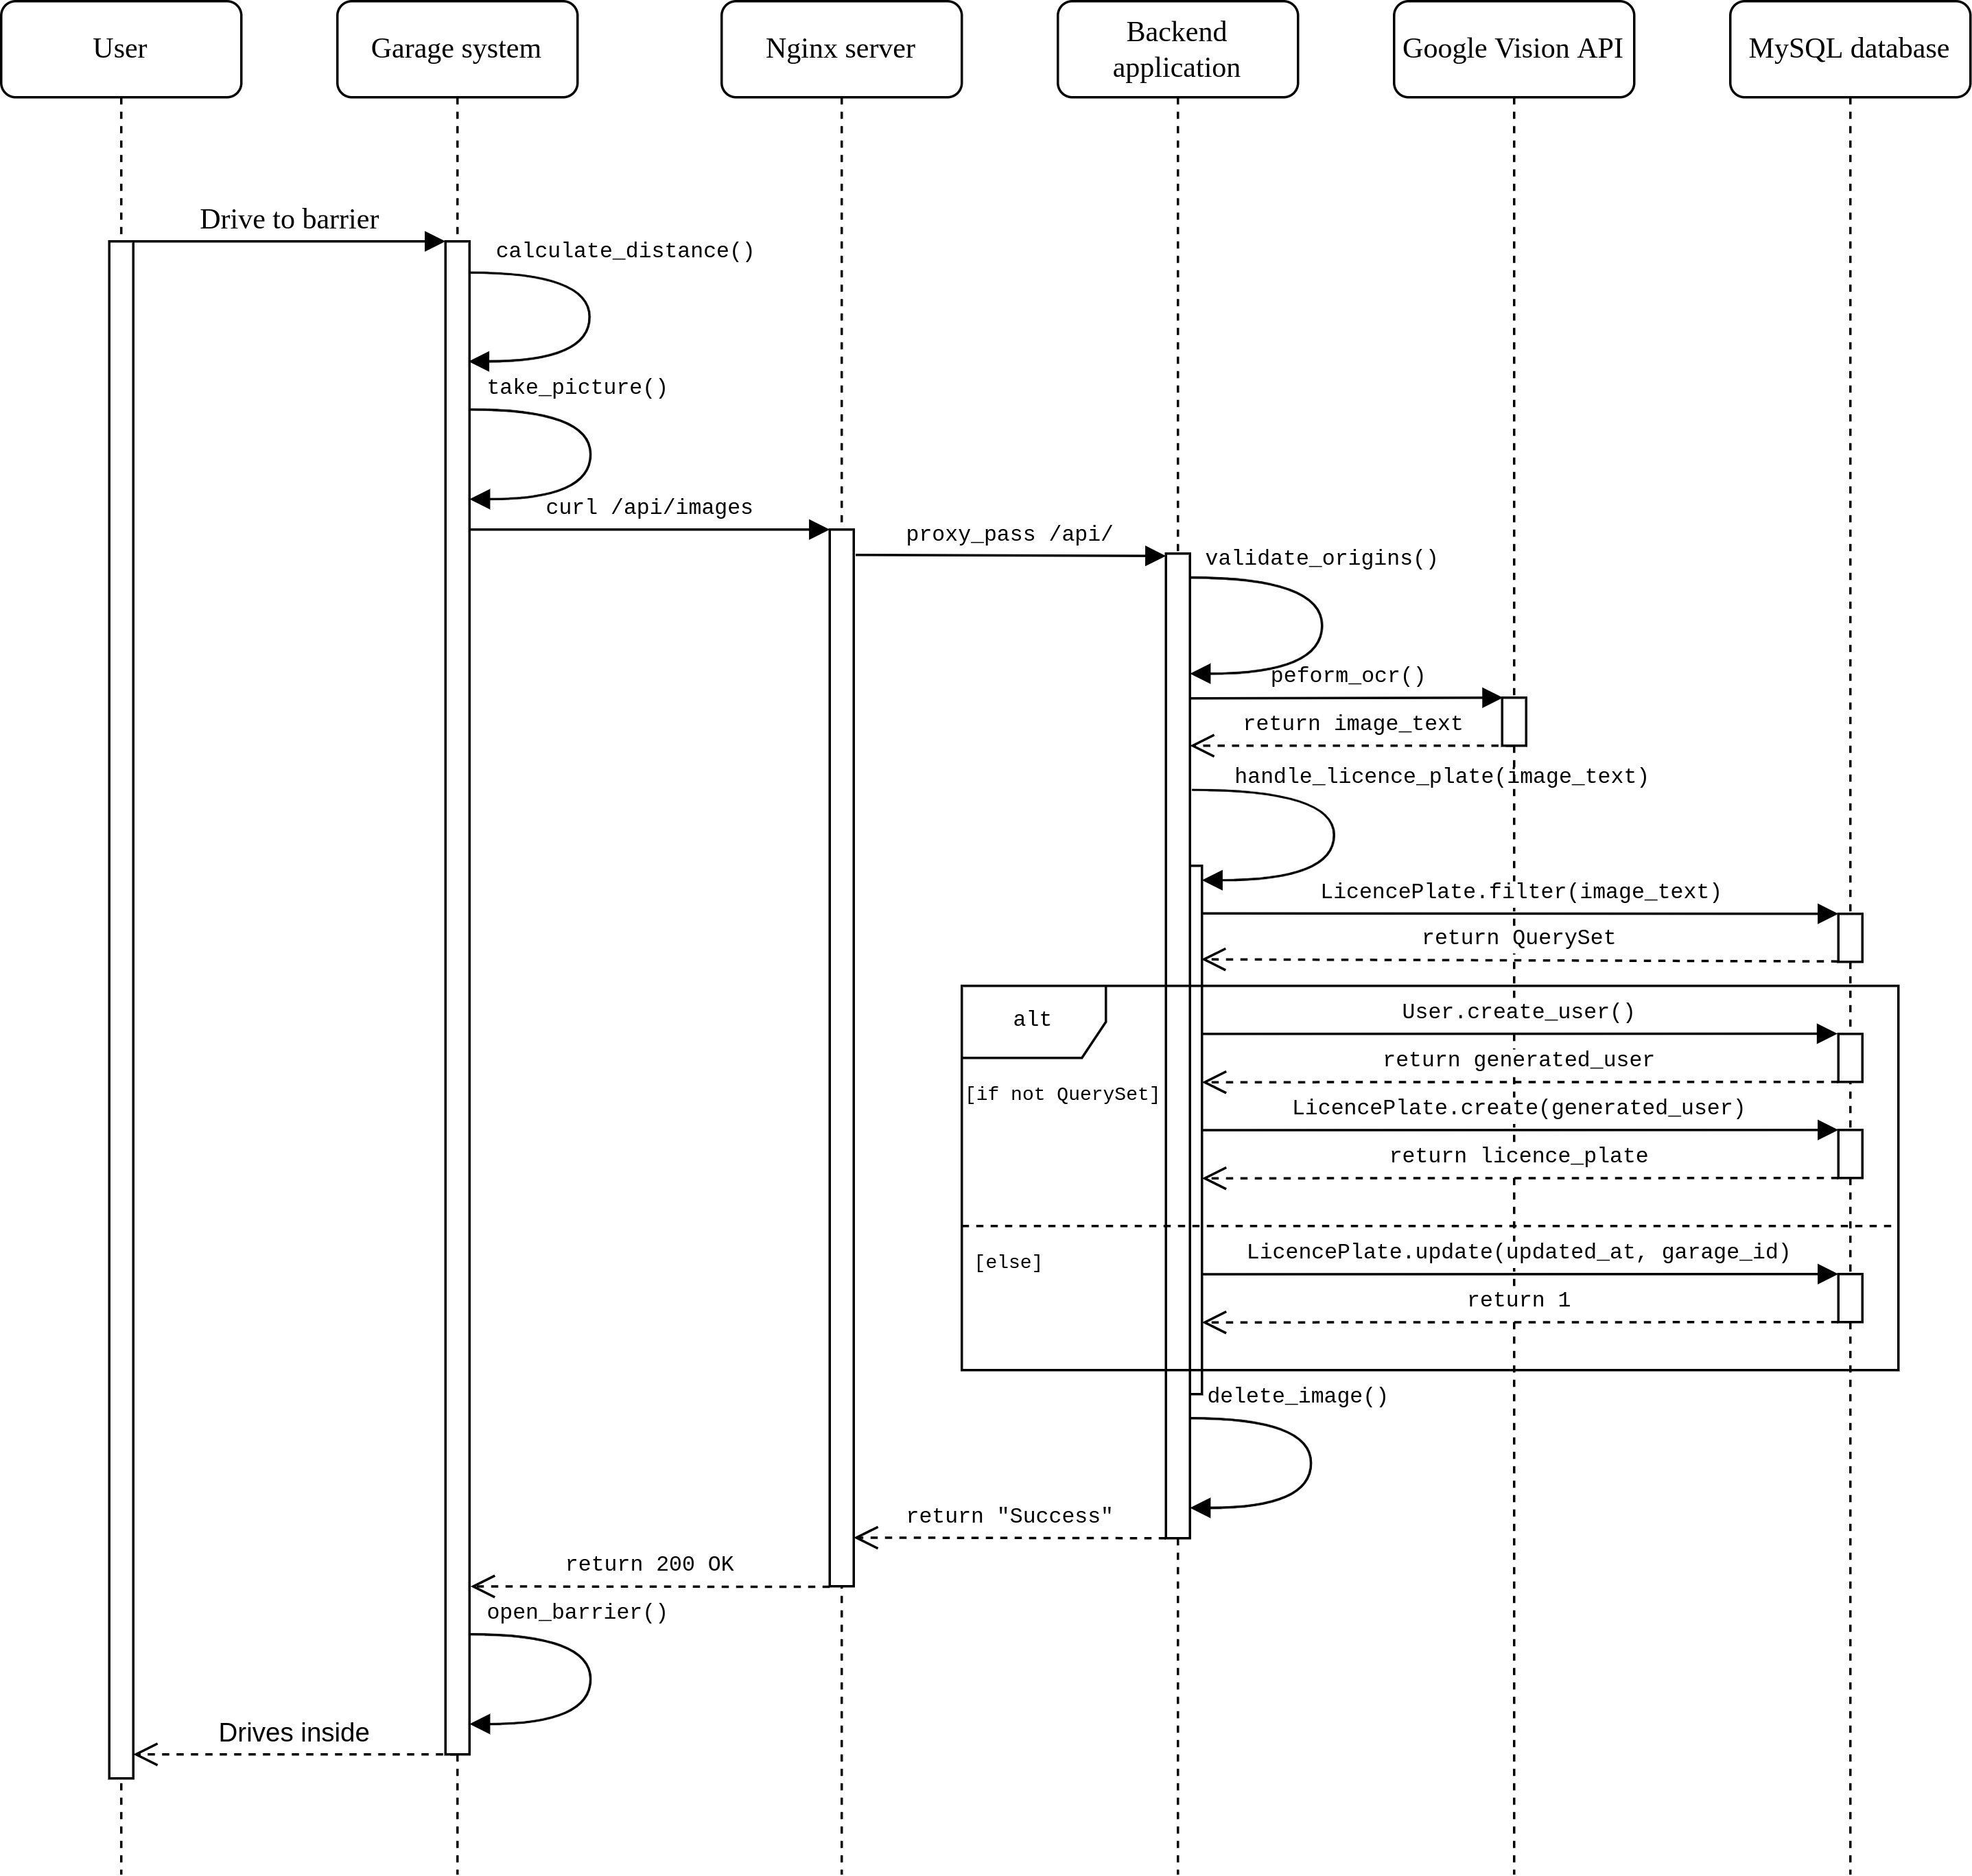
\includegraphics[width=16cm]{images/sequence_diagrams/sequence_diagram_licence_plate.drawio.png}
    \caption{Sequence diagram of the licence plate registration in the local garage system.}
    \label{fig:sequence-diagram-licence-plate}
\end{figure}

\begin{figure}[!hpt]
    \centering
    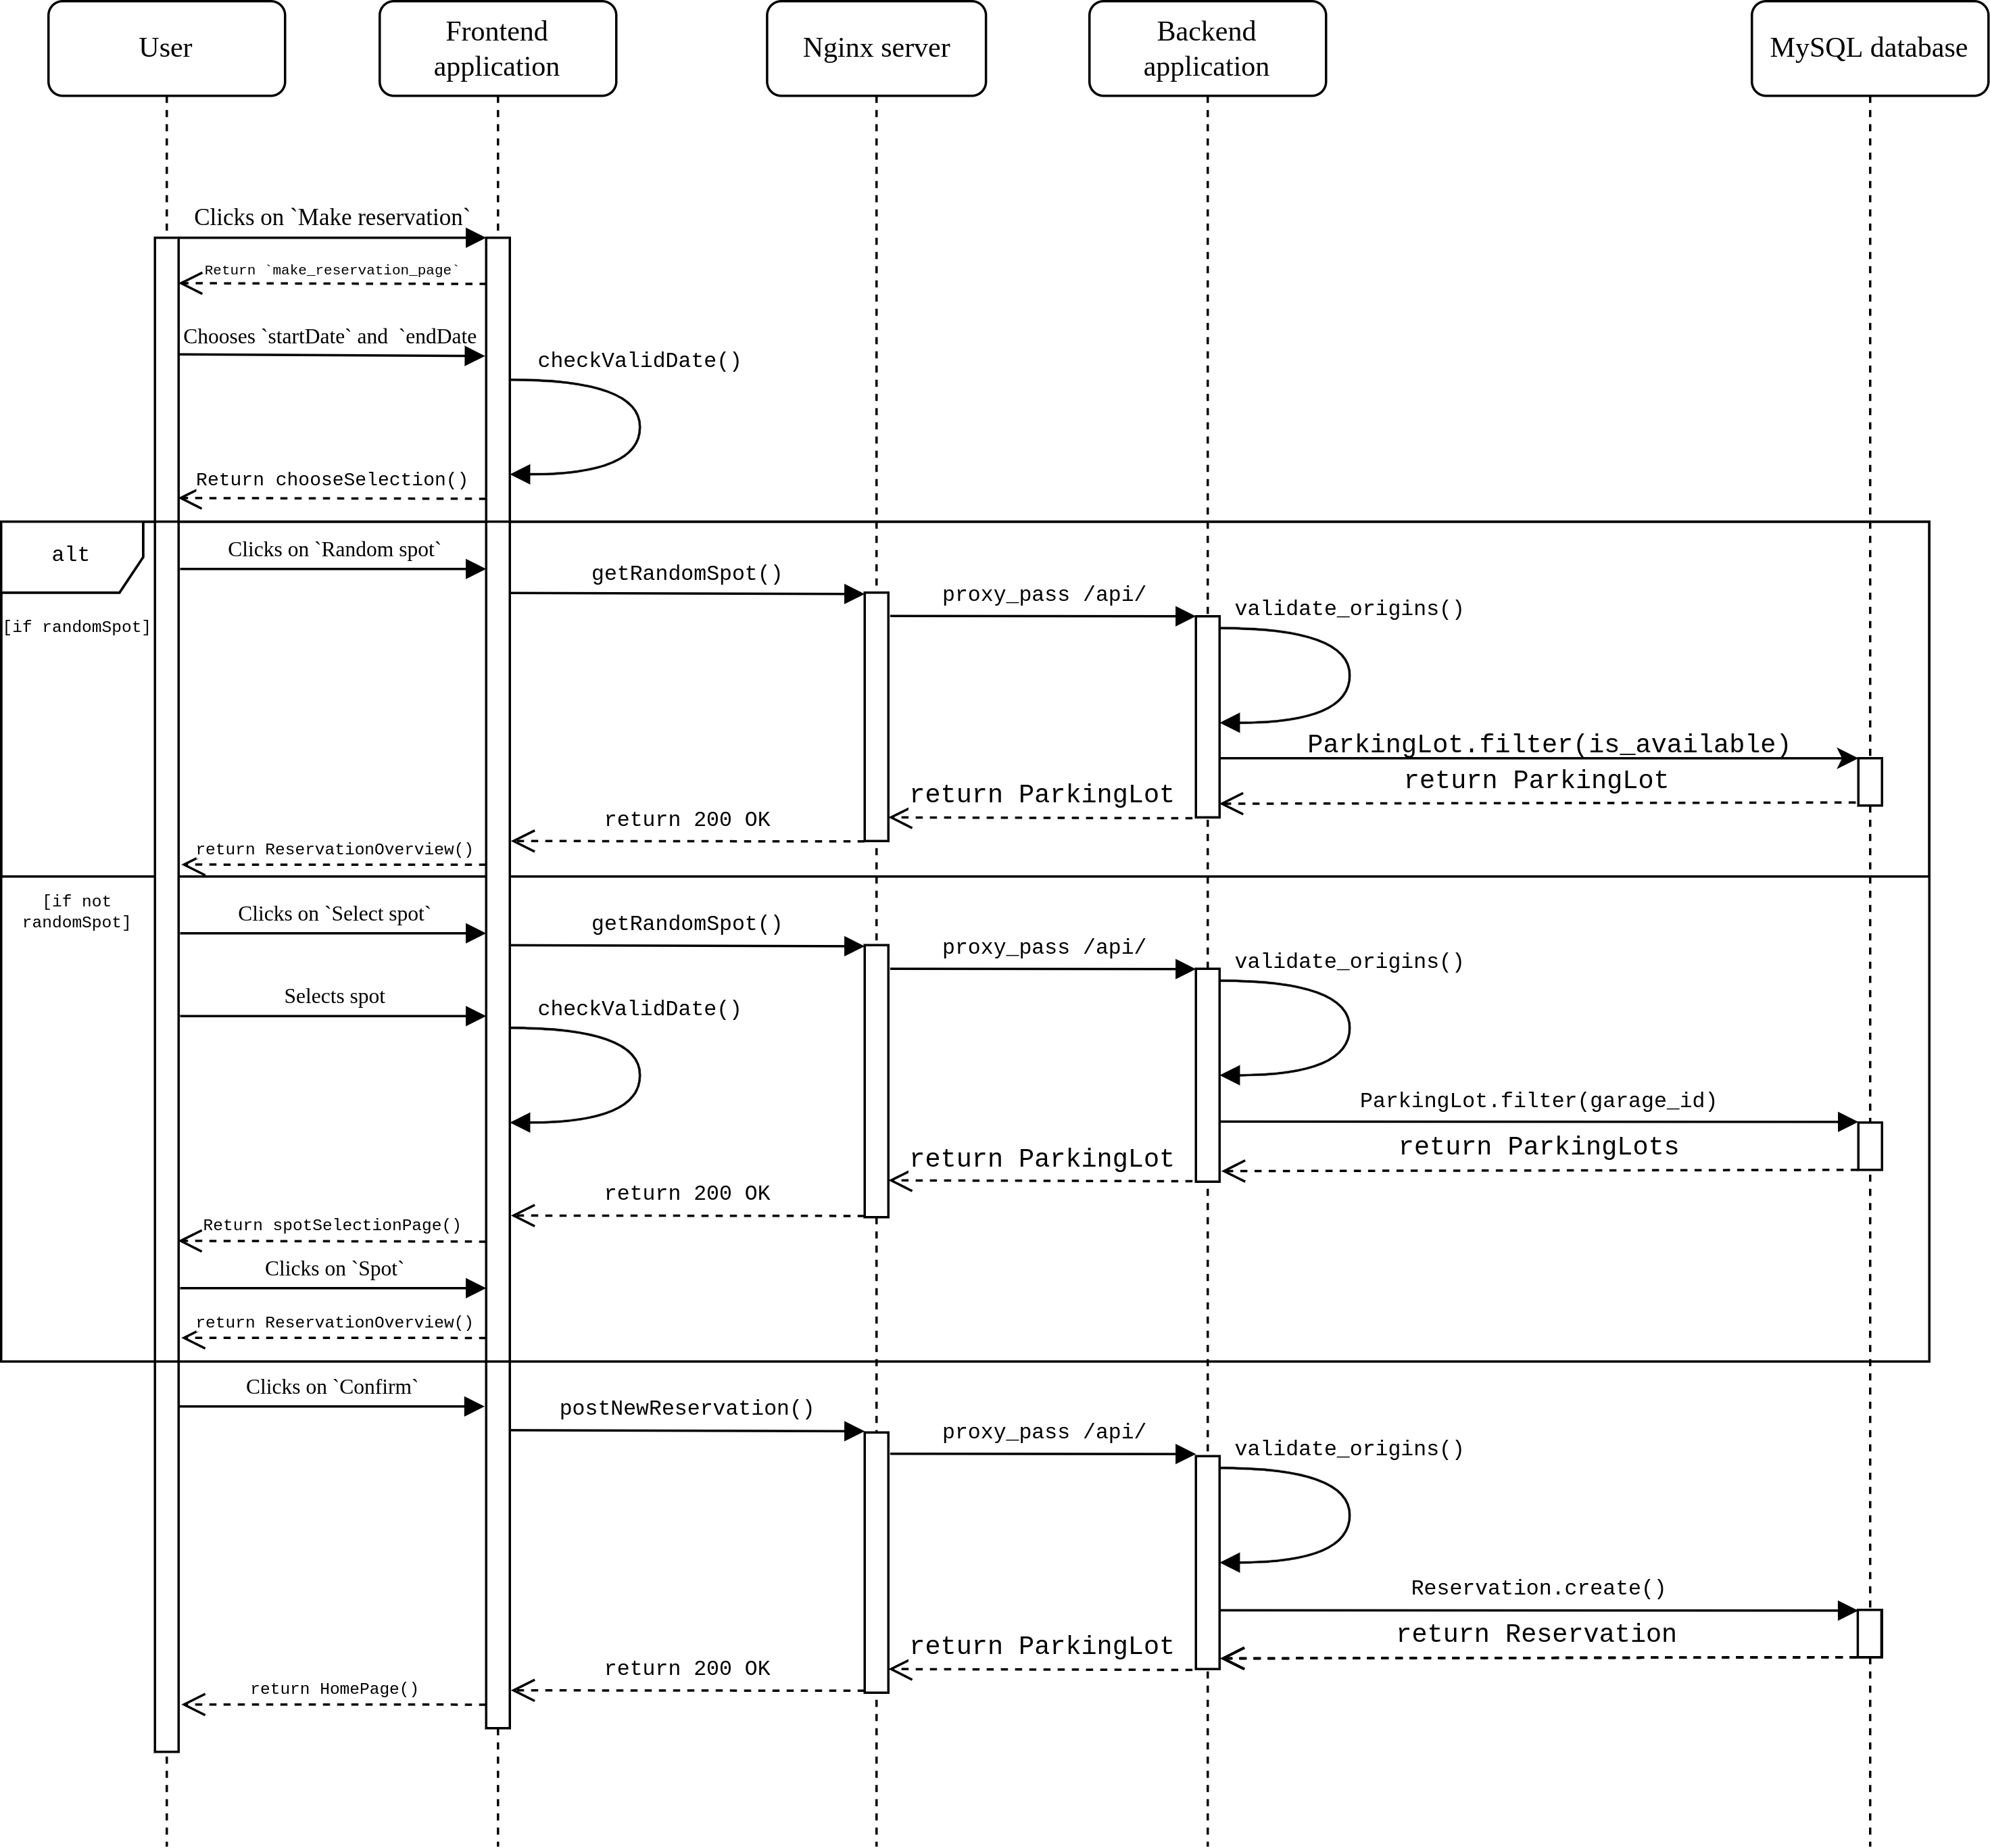
\includegraphics[width=16cm]{images/sequence_diagrams/sequence_diagram_reservation.drawio.png}
    \caption{Sequence diagram of the reservation flow.}
    \label{fig:sequence-diagram-reservation}
\end{figure}
\clearpage

\begin{figure}[!hpt]
    \centering
    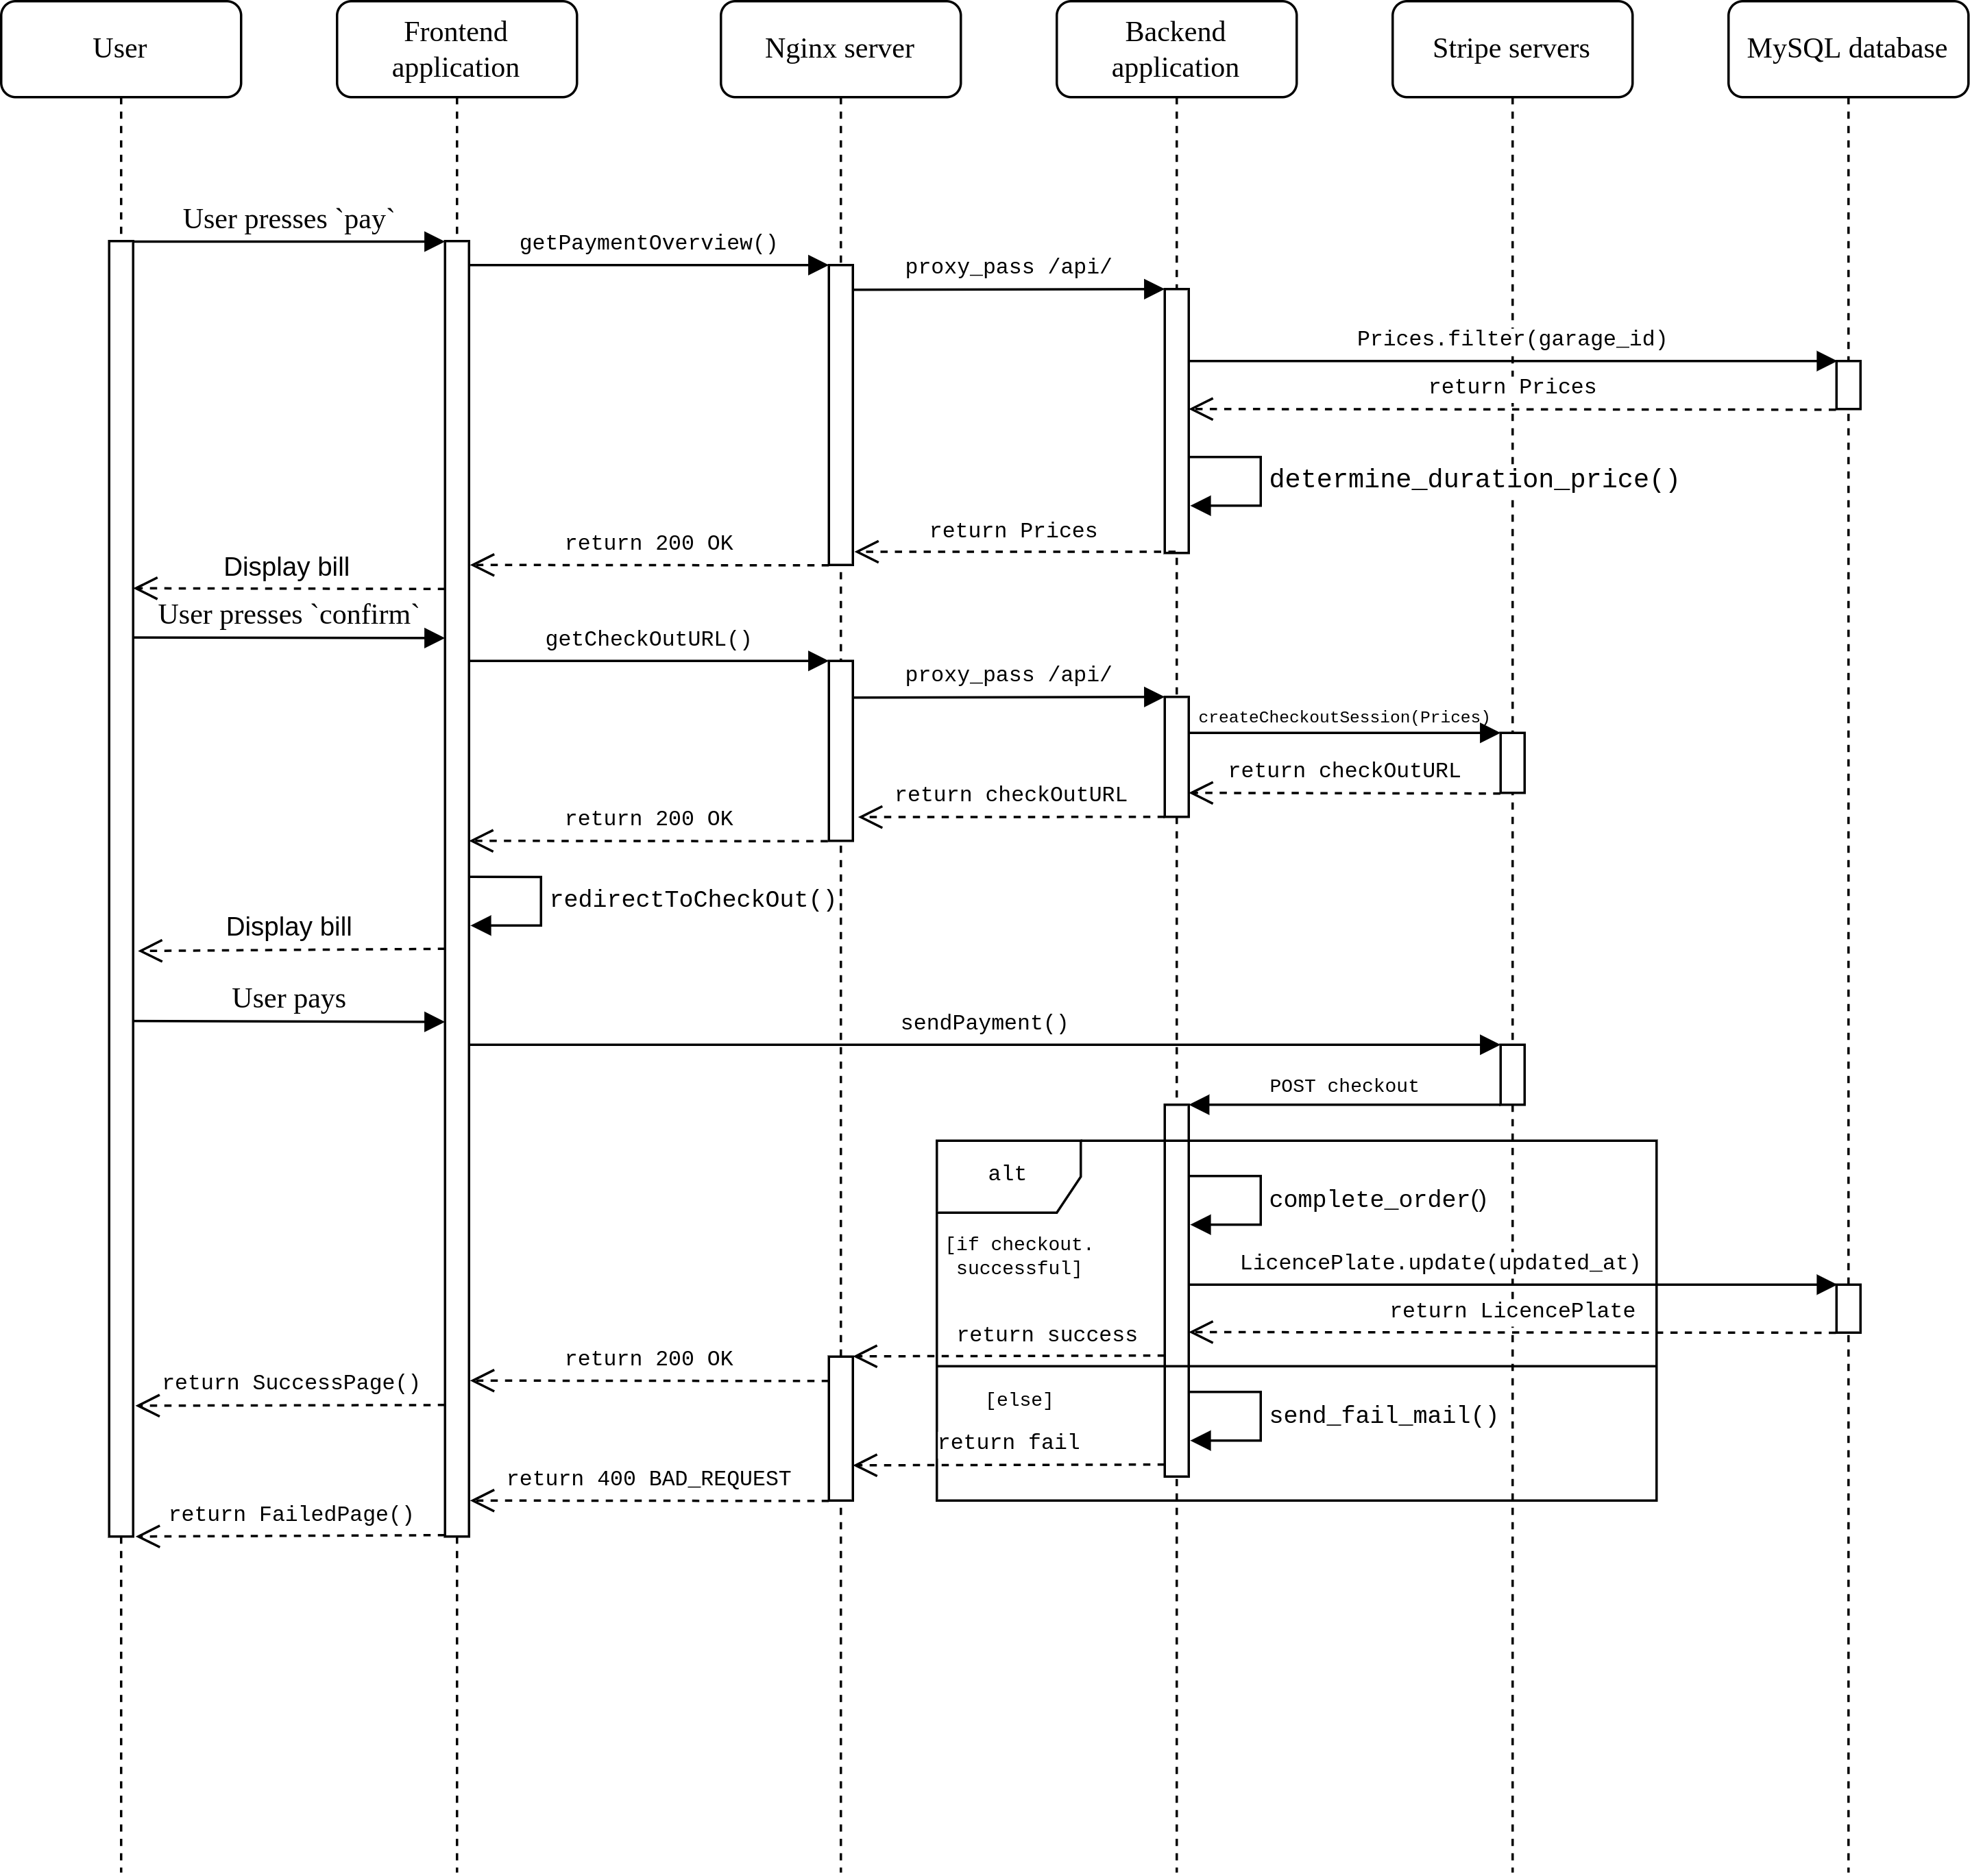
\includegraphics[width=16cm]{images/sequence_diagrams/sequence_diagram_manual_payment.png}
    \caption[Sequence diagram of the manual payment]{Sequence diagram of a manual payment. Note that this represents a payment without errors.}
    \label{fig:manual-payment}
\end{figure}

\begin{figure}[!hpt]
    \centering
    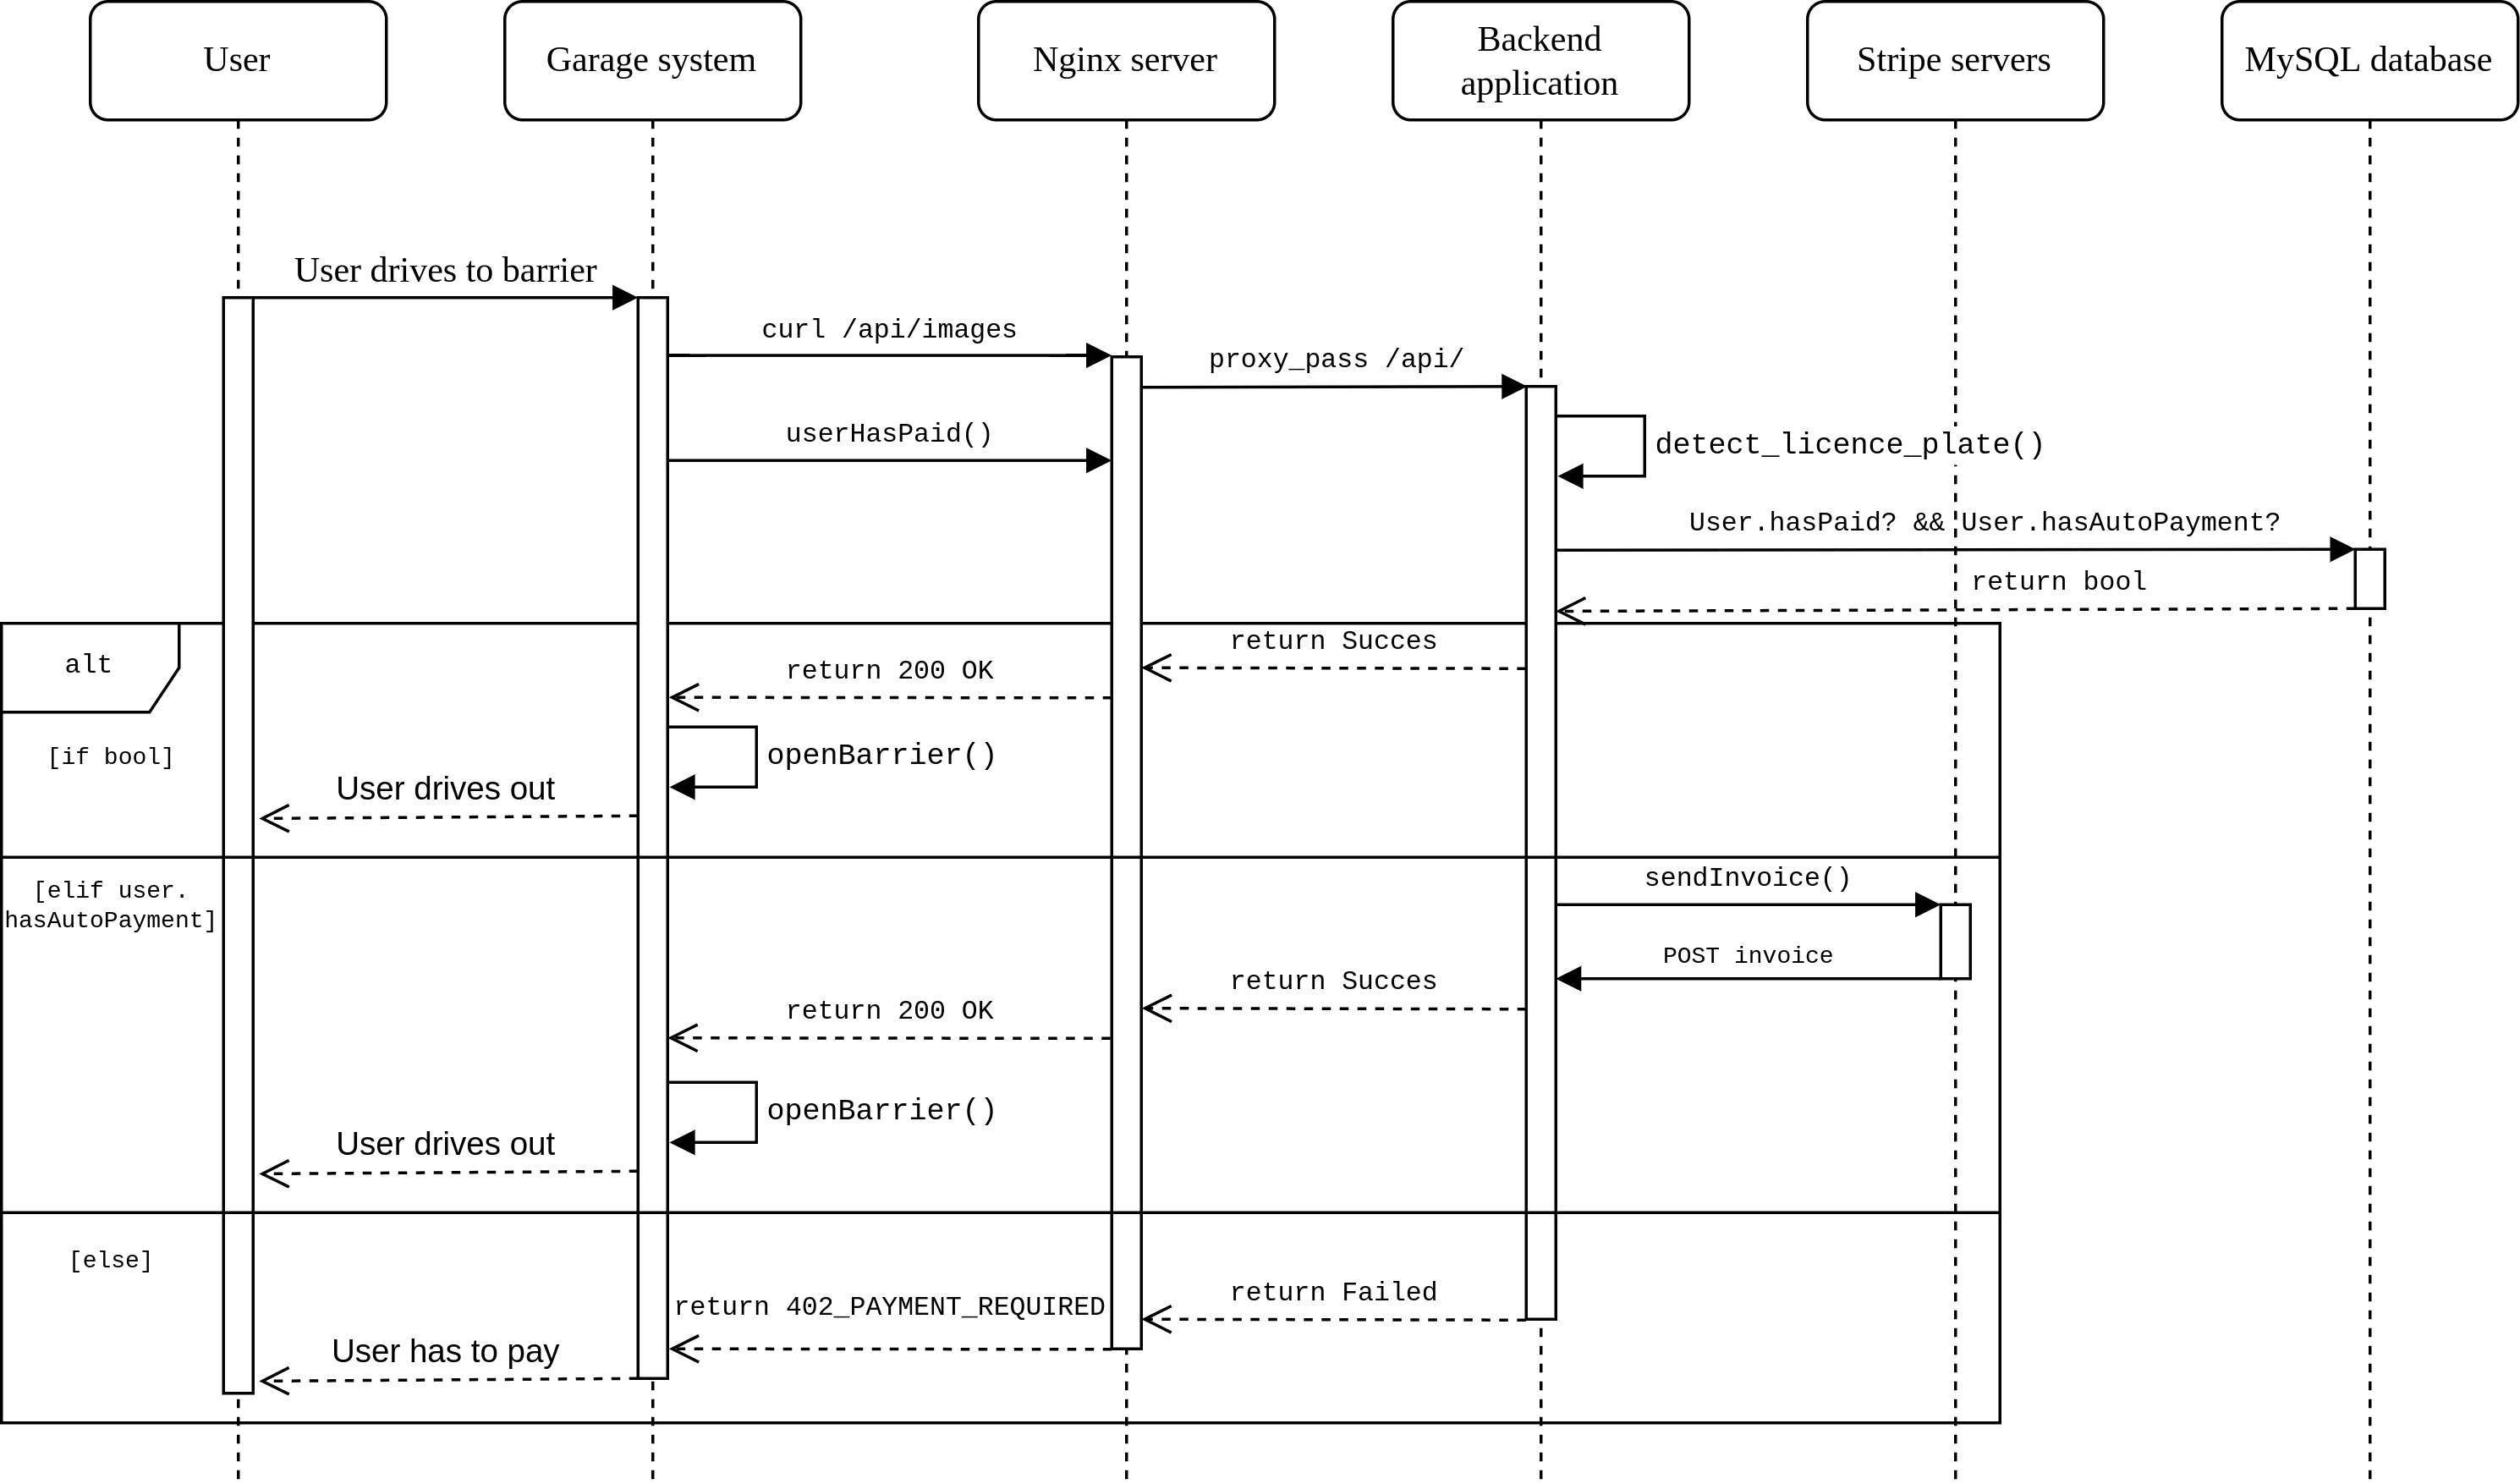
\includegraphics[width=16cm]{images/sequence_diagrams/sequence_diagram-automatic_payment.jpg}
    \caption[Sequence diagram of the automatic payment]{Sequence diagram of a automatic payment. Note that this represents a payment without errors. The \texttt{detect-licence-plate()}-function is implemented with the sequence diagram of Figure 19.}
    \label{fig:automatic-payment}
\end{figure}


\clearpage
\section{Flowcharts}\label{app:flowcharts}

\begin{figure}[htp]
    \centering
    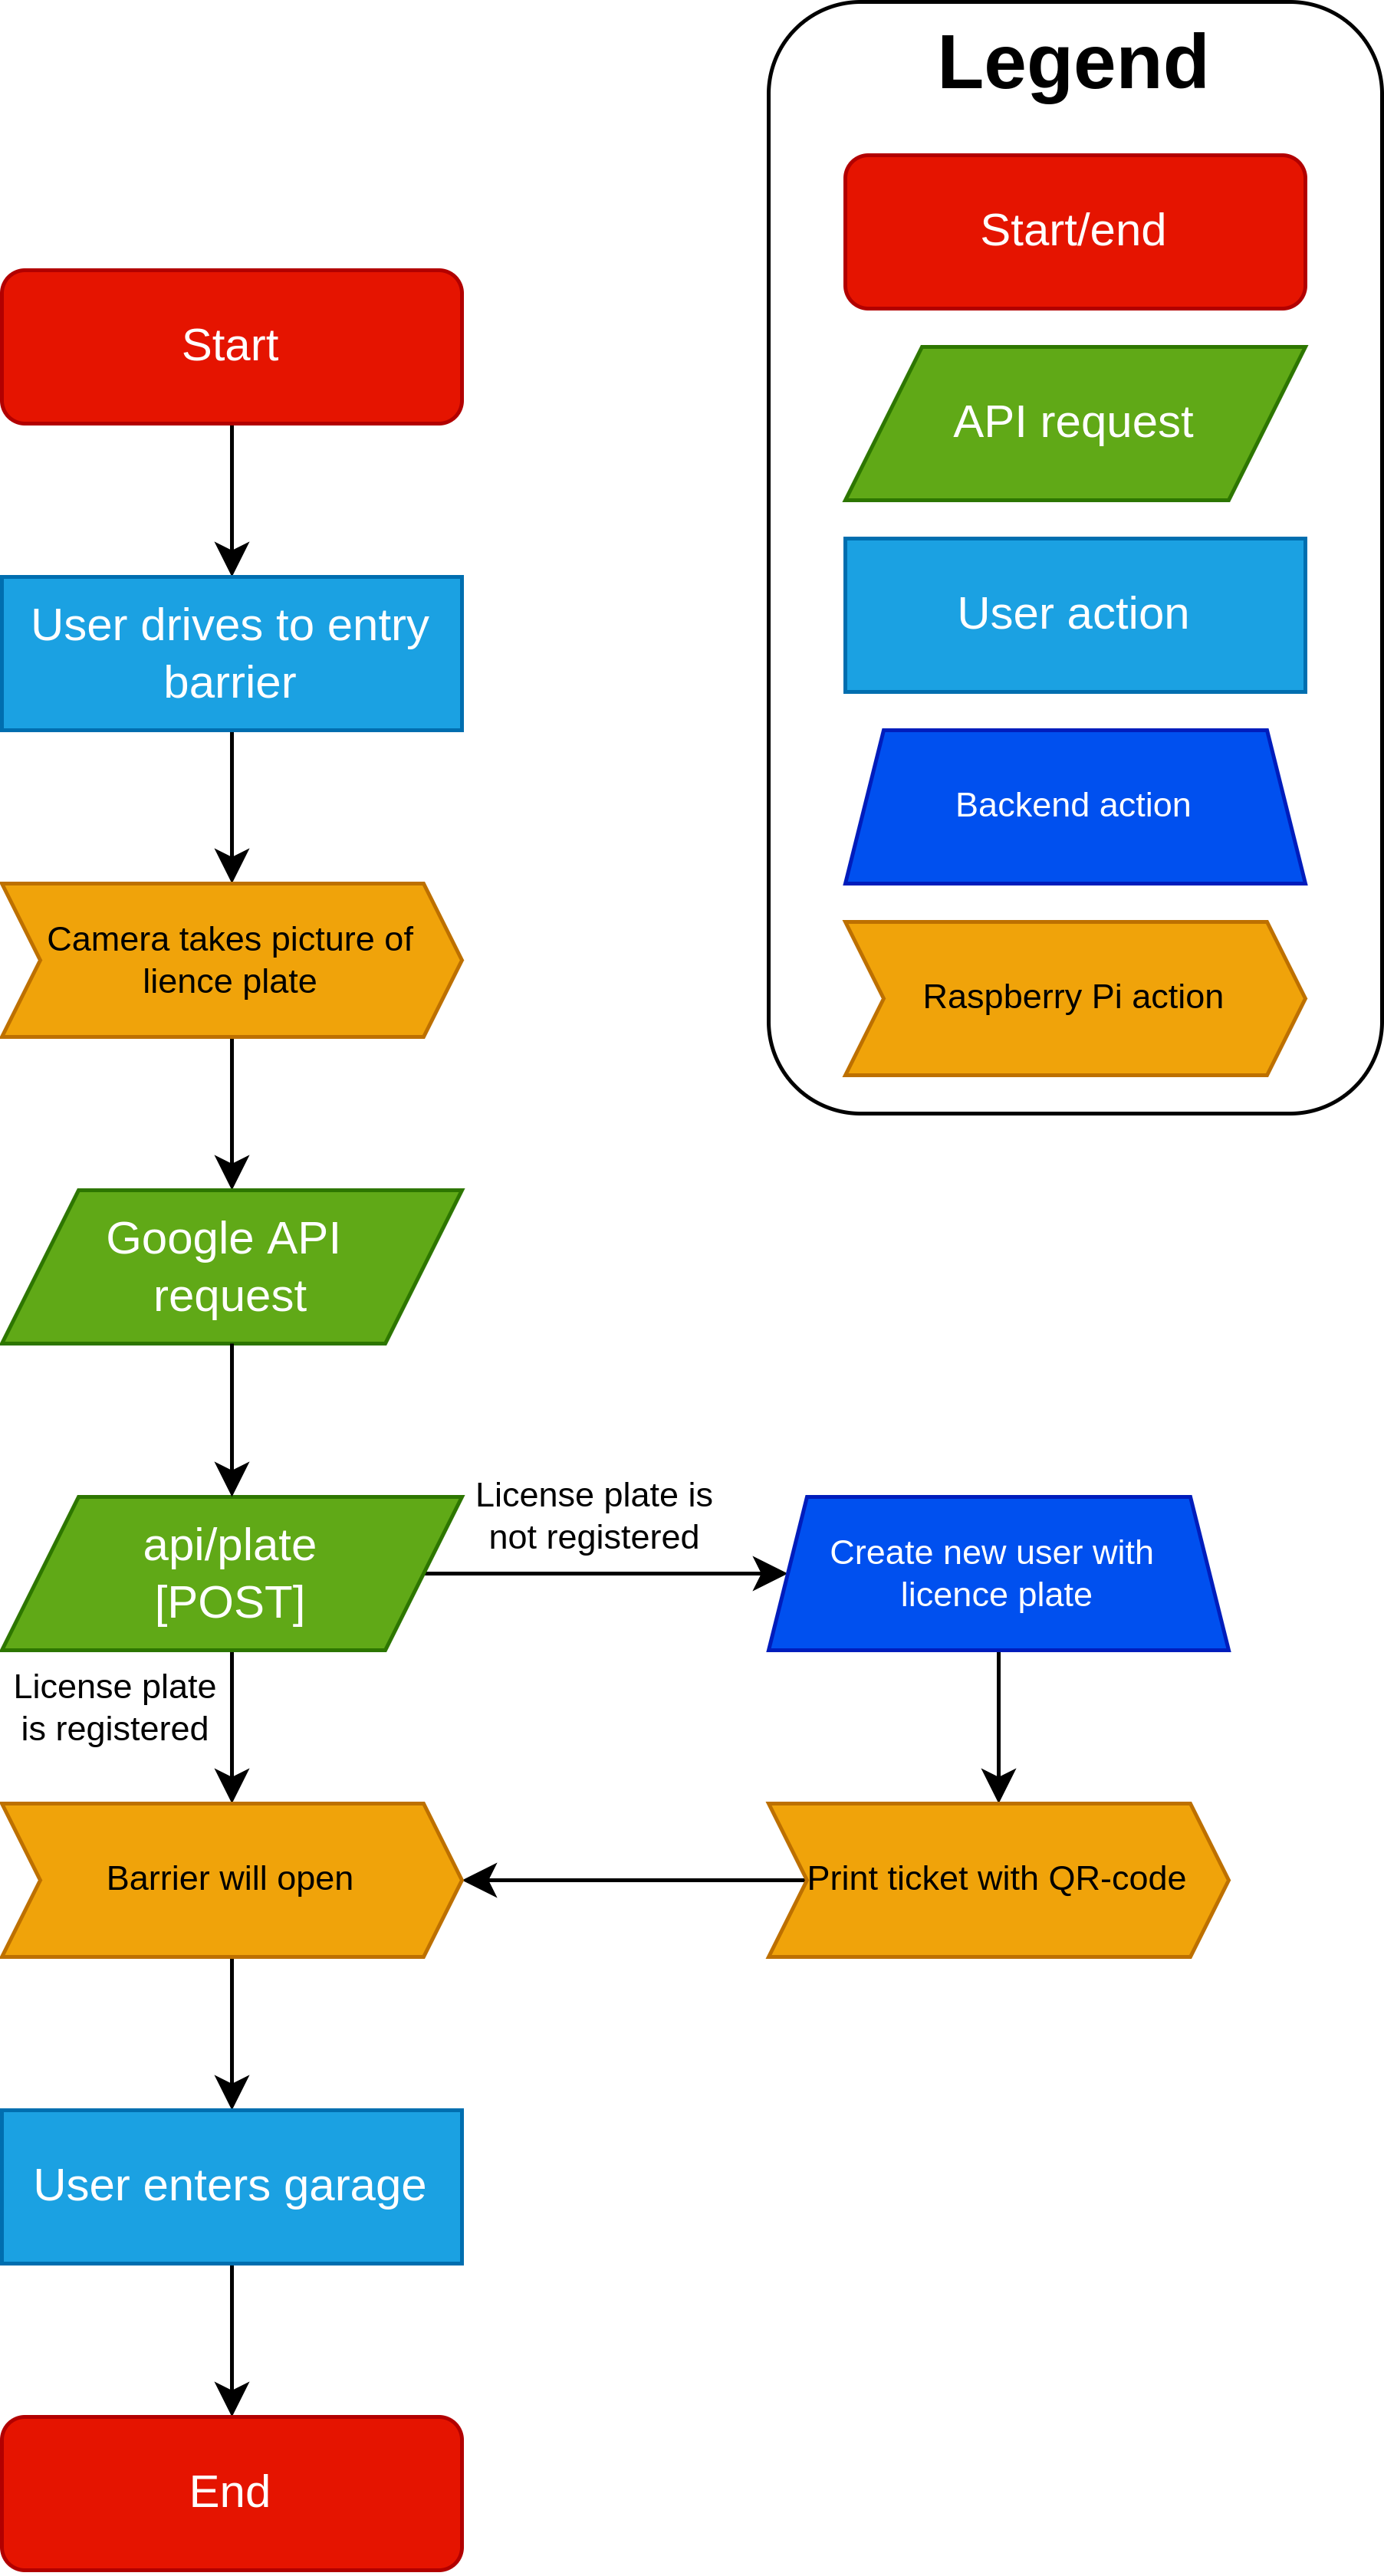
\includegraphics[width=7cm]{images/flowcharts/garage_enter.drawio.png}
    \caption{Flowchart of the entering process of the garage in both hardware, software and user terms.}
    \label{fig:garage-enter}
\end{figure}

\begin{figure}[htp]
    \centering
    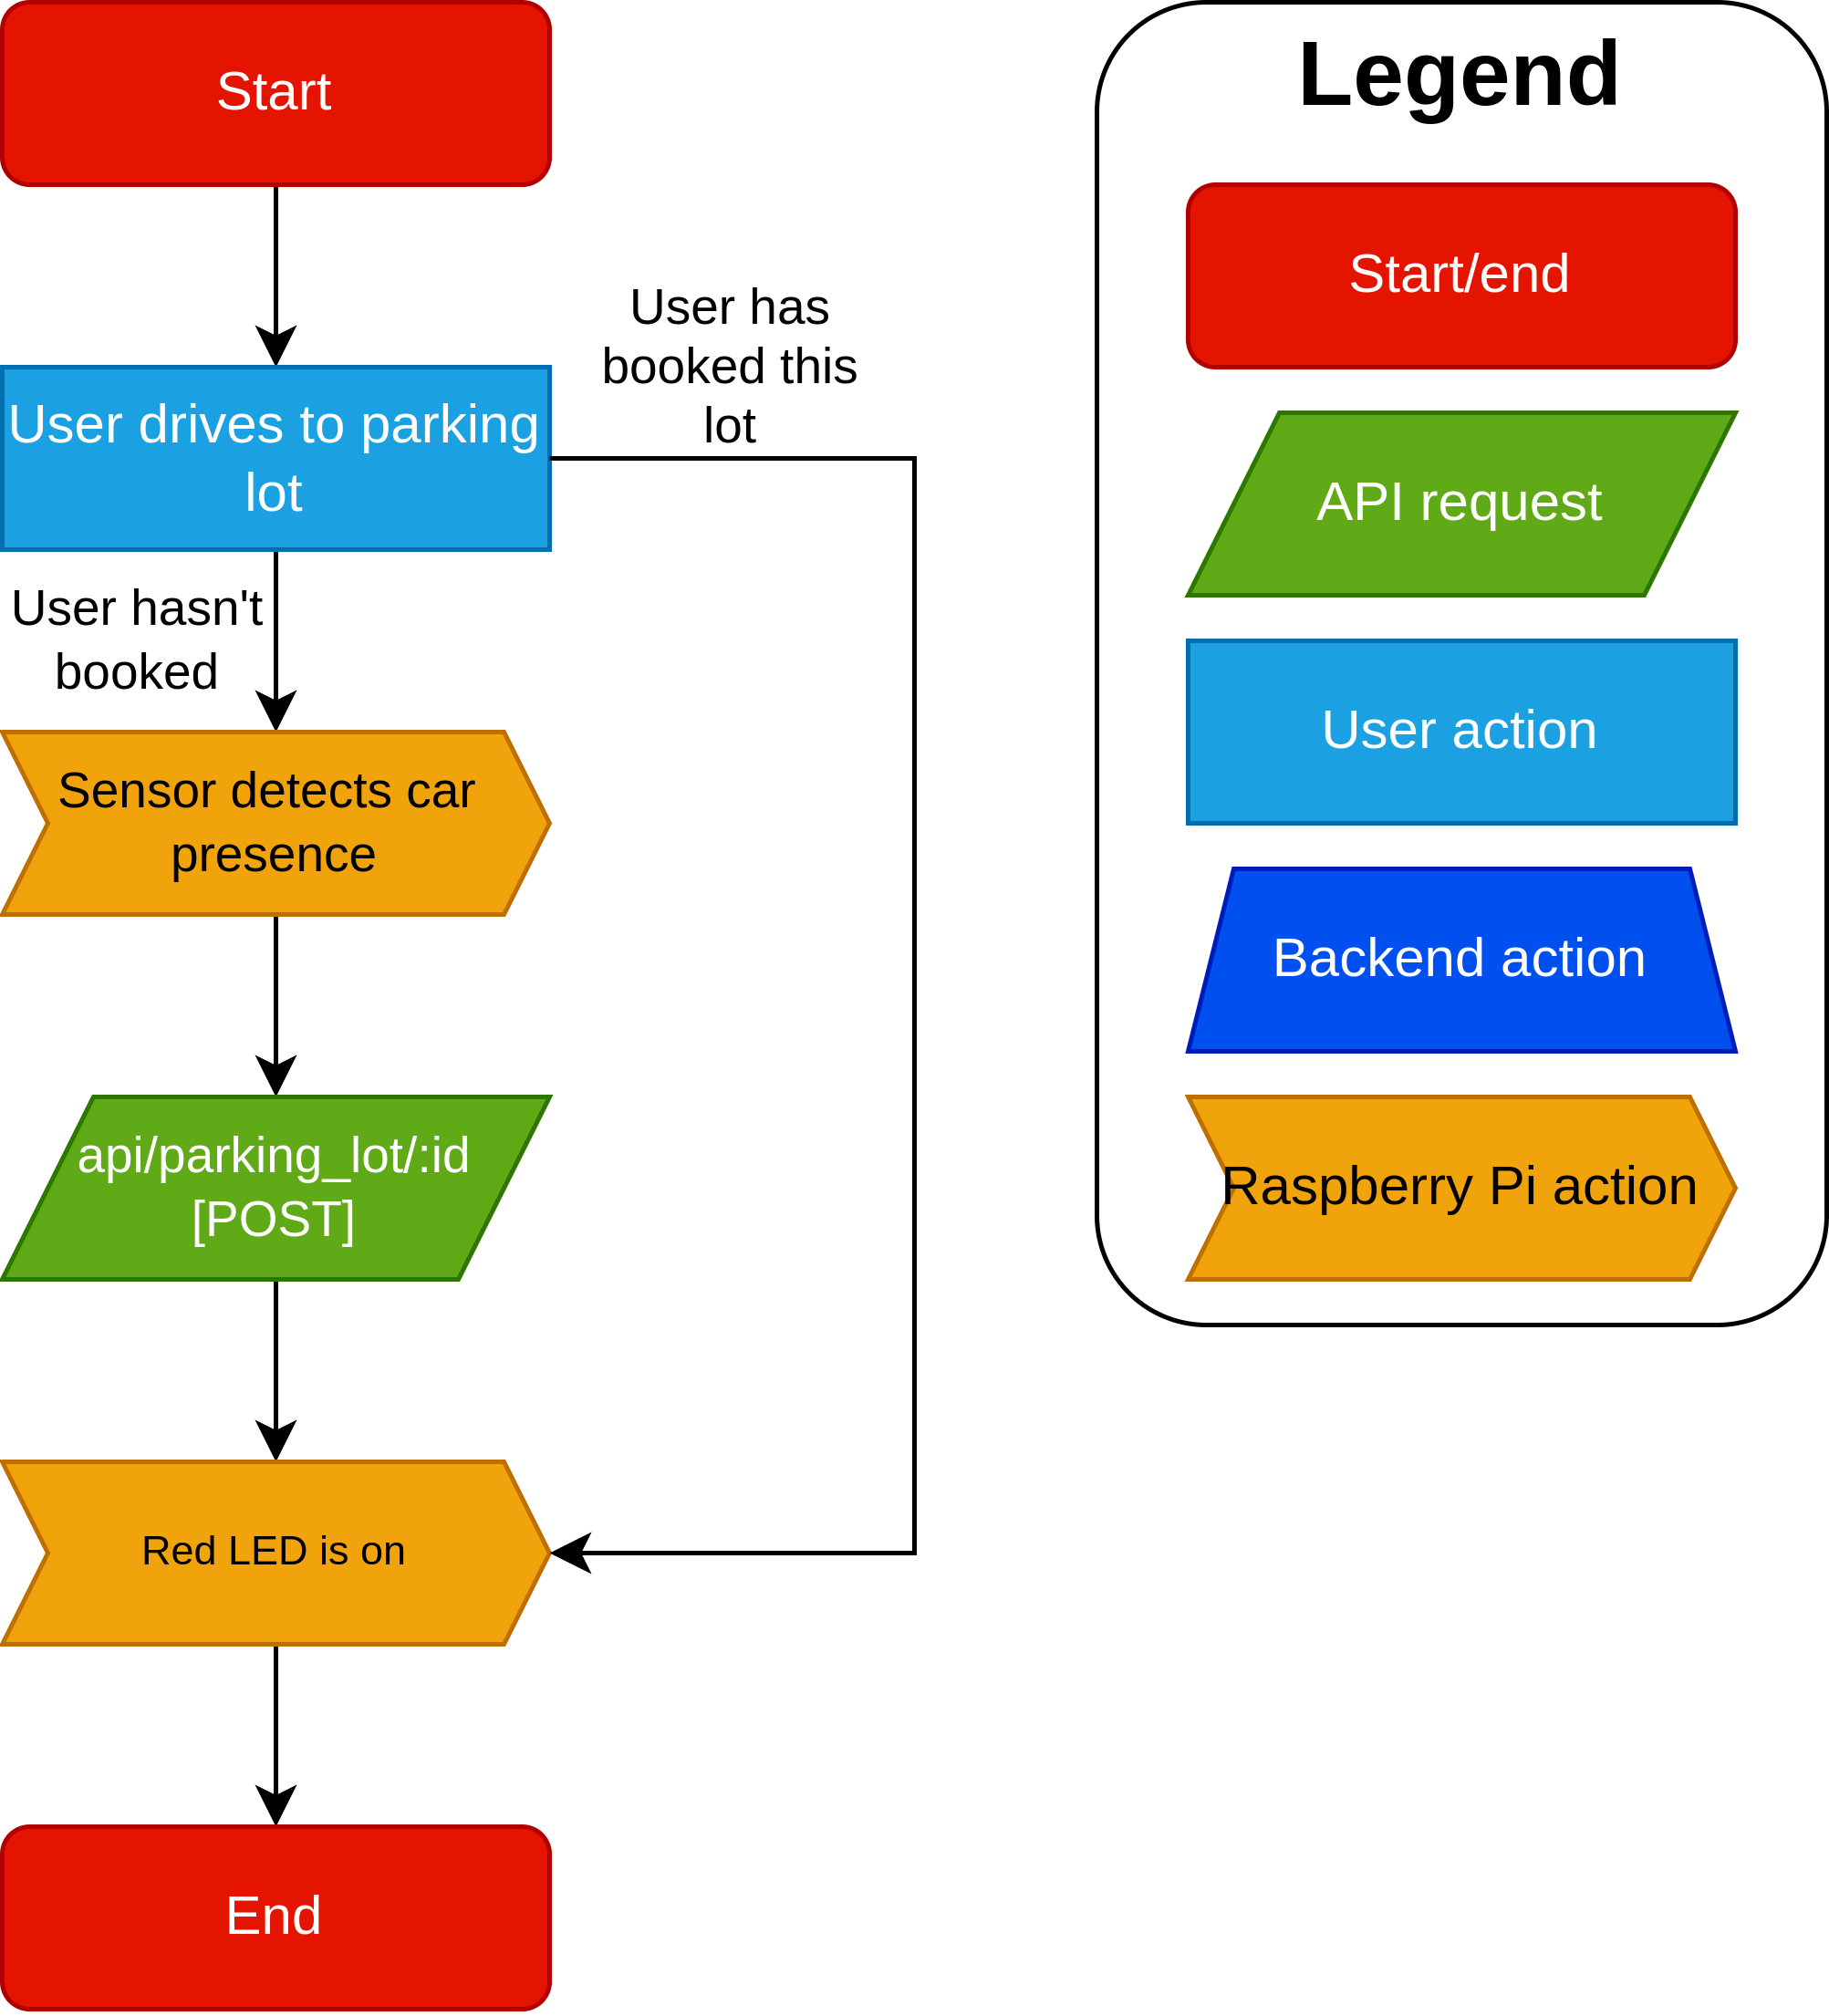
\includegraphics[width=7cm]{images/flowcharts/car_detection.drawio.png}
    \caption{Flowchart of the car detection process of the garage in both hardware, software and user terms.}
    \label{fig:car-detection}
\end{figure}

\begin{figure}[htp]
    \centering
    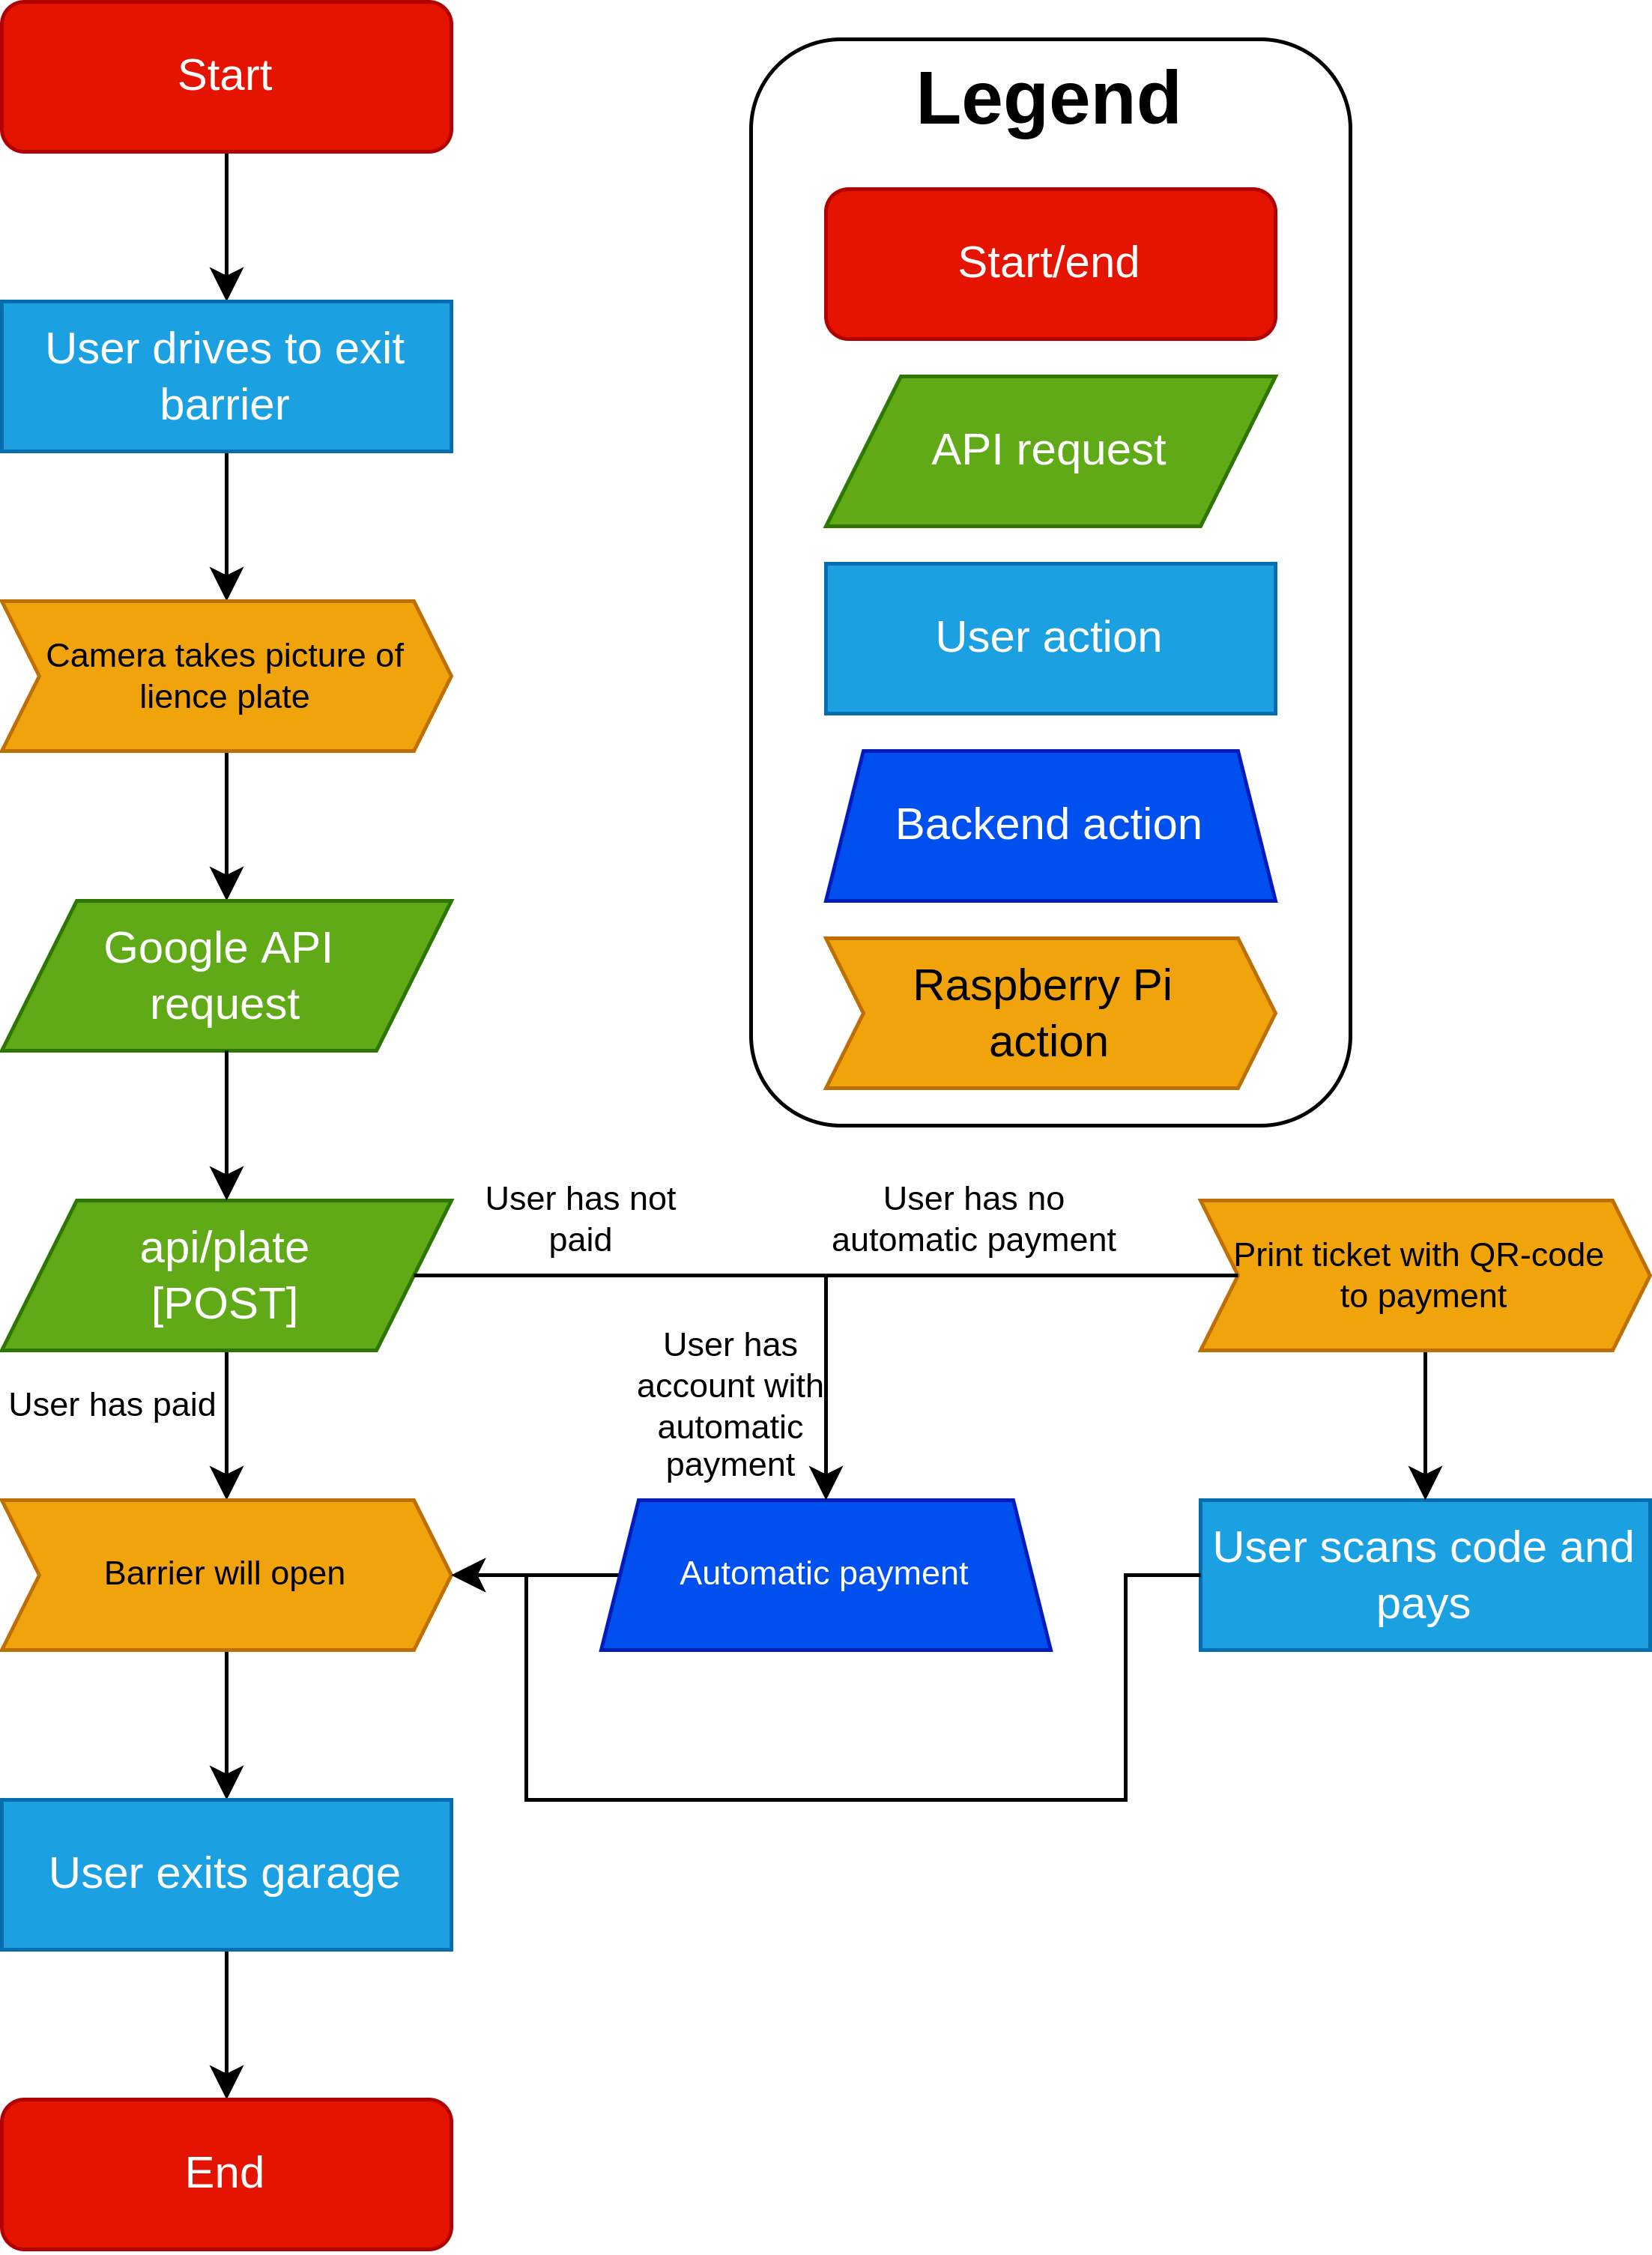
\includegraphics[width=8cm]{images/flowcharts/garage_exit.drawio.png}
    \caption{Flowchart of the exiting process of the garage in both hardware, software and user terms.}
    \label{fig:garage-exit}
\end{figure}


\end{appendices}
\end{document}
